\documentclass[../main.tex]{subfiles}
\graphicspath{{\subfix{../IMAGES/}}}

\begin{document}
\localtableofcontents
\subsection{Introduction}
\begin{itemize}
    \item Monde analogique : grandeurs à valeurs continues. Représentation continue de l'information\\
    \item Monde numérique : grandeurs à valeurs discrètes. Représentation binaire de l'information\\
\end{itemize}

Les composants électroniques se divisent en deux catégories : \\
\begin{itemize}
    \item Les composants \textbf{passifs} : Résistances, Condensateurs, Inductances. Constitués de métaux et de couches isolantes\\
    \item Les composants \textbf{actifs} : Diodes, Transistors. Constitués de matériaux semi-conducteurs tels que le silicium\\
\end{itemize}

\underline{Propriétés des semi-conducteurs :} un cristal semi-conducteur à l'état pur est un matériaux relativement isolant. Sa résistance diminue si la température augmente. \textbf{De plus, la résistivité d'un semi-conducteur diminue grandement en introduisant des atomes étrangers dits dopant.}\\

Deux types de dopage :\\
\begin{itemize}
    \item Dopage de type P : atome de Bore en substitution (il manque un électron au cristal). Un "trou"\\
    \item Dopage de type N : atome de Phosphore en substitution (ajoute un électron au cristal). Un électron supplémentaire.\\
\end{itemize}

\subsection{Base d'analyse des circuits}
\subsubsection{Rappels}
\begin{itemize}
    \item Tension [Volts] $U_A> U_B \Rightarrow U_{AB} = U_A-U_B$\\
    \item Courant [Ampères] $I = \frac{dq}{dt}$ (débit de charges en coulombs/sec) \warning Dans le même sens que la tension dans un composant.\\
\end{itemize}

Convention : \begin{itemize}
    \item Grandeur variable dans le temps se note en minuscule, u\\
    \item Grandeur constante dans le temps se note en majuscule avec l'indice '0', $U_0$\\
    \item Une tension/courant est la somme d'une composante continue et d'une composante variable. On note une telle grandeur par une majuscule, U
\end{itemize}

Éléments de base : \begin{itemize}
    \item \underline{Résistance} : dans une résistance, le courant s'écoule du potentiel le plus 'haut' vers le plus 'bas', $\mathbf{U_{AB} = RI}$\\
    \item \underline{Condensateur} : il agit comme un réservoir de charges. Le courant peut avoir deux sens opposés pour une même polarisation (suivant s'il se charge, dans le même sens, ou non, inverse), $\mathbf{Q = CU_{AB}}$ (Rappel : $C = \varepsilon_R \varepsilon_0 \frac{S}{d}$ où S est la surface des électrodes et d la distance qui les sépare\\
    \item \underline{Inductance} : la tension qui se développe tend à maintenir le courant initial dans l'inductance. $\mathbf{U_{AB} = L \frac{dI}{dt}}$. Si $\phi$ est le flux du champ magnétique créé par un courant I alors $L = \frac{\phi}{I}$. De plus $L = \frac{\mu_0 \mu_R N^2S}{L}$(N le nombre de spires, S la section de l'induction et L sa longueur, $\mu_R$ et $\mu_0$ la permittivité relative et absolue)\\
\end{itemize}

Dipôle électrique : définition et convention\\
Un dipôle est décrit par la relation liant le courant i à la tension u : $u(t) = F[i(t)]$\\
\begin{itemize}
    \item La \textbf{puissance instantanée (Watts)} : $p(t) = u(t)i(t)$\\
    \item La \textbf{puissance moyenne absorbée durant une période T} : $P = \frac{1}{T} \int_0^T u(t)i(t)dt$\\
\end{itemize}
\warning Par convention, la puissance est positive si elle est absorbée et négative si elle est fournie.\\

Réécriture de la puissance moyenne : \begin{itemize}
    \item \textbf{Courant efficace} : \begin{equation}
        I_{eff} = \sqrt{\frac{1}{T} \int_0^T I(t)^2dt}
    \end{equation}
    \item \textbf{Tension efficace} : \begin{equation}
        U_{eff} = \sqrt{\frac{1}{T} \int_0^T U(t)^2dt}
    \end{equation}
\end{itemize}
La puissance moyenne est dès lors : \begin{equation}
    P = RI_{eff}^2 = \frac{1}{R} U_{eff}^2
\end{equation}
(On a ici effectuer un "root mean square" ou "rms" pour calculer la valeur efficace)\\

Dipôles linéaires passifs : \begin{itemize}
    \item Résistance R : $p(t) = \frac{u(t)^2}{R} = R i(t)^2$, $P = R \frac{1}{T} \int_0^T i(t)^2dt = \frac{1}{R} \frac{1}{T} \int_0^T u(t)^2dt$\\
    \item Capacité C : la capacité emmagasine l'énergie sous forme électrique lors d'une charge \begin{equation}
        W(t) = \int_0^t u(t)dq = \frac{1}{2}Cu(t)^2
    \end{equation}
    \item Inductance L : énergie dans une inductance \begin{equation}
        W(t) = \int_0^t i(\tau) u(\tau)d\tau = \frac{1}{2} L(i(t)^2-i(0)^2)
    \end{equation}
    L'énergie est stockée dans le milieu magnétique traversé par les lignes de champ. 
\end{itemize}

\underline{Source de tension (idéale) :}\\
Elle impose une tension à ses bornes, qui ne dépend pas du courant qui la traverse. \begin{itemize}
    \item Source indépendante : la tension ne dépend d'aucune autre grandeur du circuit\\
    \item Source dépendante/commandée : la tension est fonction d'une autre grandeur du circuit\\
\end{itemize}

\underline{Source de courant (idéale) :}\\
Elle impose un courant qui idéalement ne dépend pas de la tension à ses bornes.\begin{itemize}
    \item Source indépendante : le courant ne dépend d'aucune autre grandeur du circuit\\
    \item Source dépendante : le courant est fonction d'une autre grandeur du circuit\\
\end{itemize}

\subsubsection{Loi de Kirchhoff}
\underline{Loi des mailles} : 
Dans une maille (boucle), la somme des chutes de tension est nulle.

\underline{Loi des noeuds} : 
La somme des courants arrivant en un noeud est nulle. \\
\warning A haute fréquence, ce n'est pas forcément respecté.\\

\subsubsection{Mise en série/parallèle}
Dipôles passifs en série : \begin{itemize}
    \item Résistance : $R_{eq} = \sum R_i$\\
    \item Capacité : $C_{eq}^{-1} = \sum (C_i)^{-1}$\\
    \item Inductance : $L_{eq} = \sum L_i$\\
\end{itemize}

Dipôles sources en série : associations de sources de tension en séries $U_{eq} = \sum U_i$\\
\warning Ne pas mettre de sources de courant en séries!\\

Dipôles passifs en parallèle : \begin{itemize}
    \item Résistance : $R_{eq}^{-1} = \sum(R_i)^{-1}$\\
    \item Capacité : $C_{eq} = \sum C_i$\\
    \item Inductance : $L_{eq}^{-1} = \sum (L_i)^{-1}$\\
\end{itemize}

Dipôles sources en parallèle : associations de sources de courant en parallèle $I_{eq} = \sum I_i$\\
\warning Ne pas mettre de sources de courant en parallèle!\\

\subsubsection{Analyse générale d'un circuit linéaire}
\quad \underline{Circuit RC passe-bas :}\\
\begin{equation}
\begin{gathered}
    u_c(t) = U_0 (1-e^{-\frac{t}{RC}})\\
    i(t) = \frac{U_0}{R} e^{-\frac{t}{RC}}\\
    \end{gathered}
\end{equation}

\quad \underline{Circuit RC passe-haut :}\\
\begin{equation}
    \begin{gathered}
        u_R(t) = U_0 e^{-\frac{t}{RC}}\\
        i_R(t) = \frac{U_0}{R} e^{-\frac{t}{RC}}\\
    \end{gathered}
\end{equation}

\quad \underline{Circuit LR :}\\
\begin{equation}
    \begin{gathered}
        i_L(t) = \frac{U_0}{R} (1-e^{-\frac{t}{(L/R)}})\\
        u_L(t) = U_0e^{-\frac{t}{(L/R)}}\\
    \end{gathered}
\end{equation}

\quad \underline{Circuit RLC série :}\\
\begin{equation}
    \begin{gathered}
        \Ddot{u}_R + \frac{\omega_0}{Q} \dot{u}_R + \omega_0^2 u_R = 0\\
        \begin{cases}
            \omega_0 = \frac{1}{\sqrt{LC}}\\
            Q = \frac{\sqrt{L/C}}{R} & \text{le facteur de qualité}\\
        \end{cases}
        \begin{cases}
            \text{si Q<1/2} & u_R(t) = \frac{U_0}{\sqrt{1-\frac{4L}{CR^2}}} (e^{-\frac{t}{\tau_1}}-e^{-\frac{t}{\tau_2}})\\
            \text{si Q> 1/2} & u_R(t) = \frac{U_0R}{\omega_L}e^{-t\frac{R}{2L}}\\
        \end{cases}
    \end{gathered}
\end{equation}
Avec \begin{itemize}
    \item $\tau = \frac{2L}{R\pm \sqrt{R^2 - 4\frac{L}{C}}}$\\
\item $\omega = \omega_0 \sqrt{1-\frac{1}{4Q^2}}$
\end{itemize}

\quad \underline{Théorème de Superposition :}\\
\begin{theorem}
    Dans un circuit linéaire, l'effet de plusieurs sources indépendantes est obtenu par la somme des effets de chaque source prise individuellement lorsque toutes les autres sont désactivées.\\
    \begin{itemize}
        \item Une source de tension désactivée correspond à une source de tension nulle : court-circuit\\
        \item Une source de courant désactivée correspond à une source de courant nul : circuit ouvert\\
    \end{itemize}
\end{theorem}

\quad \underline{Théorème de Thévenin-Norton :}\\
Tout un dipôle ne comportant que des sources et des résistances est équivalent à : \begin{itemize}
    \item une source de tension en série avec une résistance interne\\
    \item une source de courant en parallèle avec cette même résistance\\
\end{itemize}

$R_0$ est la \textbf{résistance interne} du dipôle lorsque toutes les sources indépendantes sont annulées.\\

Les équivalents de Thévenin et Norton sont toujours liés par la relation : \begin{equation}
    U_{eqT} = R_0 I_{eqN}
\end{equation}

\subsection{Régime sinusoïdal}
Un signal sinus d'amplitude $\hat{A}$, de phase initiale $\phi$ et de pulsation $\omega$ peut être décrit par un phaseur complexe $\underline{A}$ d'amplitude $\hat{A}$ et d'argument $\phi$ : $\underline{A} = \hat{A}e^{j\phi}$.\\

$u(t) = \hat{U} \sin(\omega t+ \varphi_2)$, $i(t)= \hat{I} \sin(\omega t+ \varphi_1)$\\

\quad \underline{Dipôles linéaires en régime sinus :}\\
\begin{itemize}
    \item Résistance : $\underline{U} = R\underline{I}$, $\varphi=0$\\
    \item Capacité : $\underline{U} = \frac{1}{j\omega C}\underline{I}$, $\varphi = -\frac{\pi}{2}$\\
    \item Inductance : $\underline{U} = j\omega L \underline{I}$, $\varphi = \frac{\pi}{2}$\\
\end{itemize}

\quad \underline{Impédance :}\\
\begin{equation}
    \underline{U} = \underline{Z} \underline{I}, \Omega
\end{equation}

\quad \underline{Admittance :}\\
\begin{equation}
    \underline{I} = \underline{Y} \underline{U}, \Omega^{-1}
\end{equation}

On a donc la relation : $Z = \frac{1}{Y}$\\
Les lois de Kirchhoff restent valables avec des phaseurs. \\

\begin{itemize}
    \item $Z_{serie} = \sum Z_i$\\
    \item $Z_{parallele} = \frac{1}{\sum \frac{1}{Z_i}}$\\
    \item $Y_{parallele} = \sum Y_i$\\
\end{itemize}

L'impédance complexe Z peut être décomposée en une partie réelle R (résistance > 0) et une partie imaginaire X (réactance) : $Z = R+jX$\\

La valeur crête et la valeur de l'amplitude du signal (valeur max).\\

\subsubsection{Puissance moyenne}
Pour une résistance, on a :
\begin{equation}
    P = \frac{1}{2R} \hat{U}^2 = R\frac{\hat{I}^2}{2} = \frac{U_{eff}^2}{2} = RI_{eff}^2
\end{equation}
Avec $U_{eff}$ et $I_{eff}$ respectivement la tension efficace et courant efficace : $U_{eff} = \frac{\hat{U}}{\sqrt{2}}$.\\

Sinon, de manière générale : \begin{equation}
    P = U_{eff} I_{eff} \cos(\arg(\underline{Z})) = I_{eff}^2 \Re(Z)
\end{equation}
On définit également la puissance apparente comme le maximum de P($U_{eff} I_{eff}$).\\

\subsubsection{Superposition et Thévenin/Norton}
Dans un circuit linéaire avec des sources sinusoïdales indépendantes, on peut appliqué le principe de superposition ainsi que le théorème de Thévenin/Norton. On cherche alors à trouver : \begin{itemize}
    \item Source de tension $\underline{U}_{eqT}$\\
    \item Impédance de source $\underline{Z}_s$\\
    \item Source de courant $\underline{I}_{eqN}$\\
\end{itemize}

\subsubsection{Fonction de transfert}
Dans un système linéaire, la réponse à une excitation sinusoïdale est une sinusoïdale de même fréquence avec un déphasage d'amplitude proportionnelle à l'amplitude de l'excitation.\\

\begin{equation}
    \begin{gathered}
        e(t) = H\cos(\omega t) \rightarrow s(t) = HE \cos(\omega t+\phi)\\
        \underline{S}= \underline{H} \underline{E}\\
    \end{gathered}
\end{equation}

Avec $\underline{H}$, la fonction de transfert.\\
\begin{equation}
    \underline{H}(j\omega) = \frac{\underline{S}(j\omega)}{\underline{E}(j\omega)}
\end{equation}

Critères de stabilité : \begin{itemize}
    \item les pôles ont une partie réelle négative\\
    \item le degré du dénominateur est supérieur ou égale à celui du numérateur\\
\end{itemize}

Pour $k$ sources indépendantes, on a $S(j\omega) = \sum_k J_k(j\omega) E_k(\omega)$\\

Un quadripôle linéaire est un circuit composé d'éléments linéaires avec deux bornes d'entrées auxquelles est branchée une source indépendante avec une impédance $Z_s$ et deux bornes de sortie connectées à une impédance de charge $Z_L$\\

\begin{itemize}
    \item Gain en tension : $H(j\omega) = \frac{U_{out}}{U_{in}}$\\
    \item Gain en courant : $H(j\omega) = \frac{I_{out}}{I_{in}}$\\
    \item Transimpédance : $H(j\omega) = \frac{U_{out}}{I_{in}}$\\
    \item Transadmittance : $H(j\omega)=\frac{I_{out}}{U_{in}}$\\
\end{itemize}
\warning Les courants aux deux accès du quadripôle sont définis positifs dans le sens entrant.\\

Le gain en tension change selon la nature de $Z_L$.\\

\subsubsection{Diagramme de Bode}
On représente ici $H(j\omega)$ par son module et son argument.\\
\begin{itemize}
    \item $20\log \lvert H \rvert$ vs $\log(\omega)$\\
    \item $arg(H)$ vs $\log(\omega)$\\
\end{itemize}

Si plusieurs fonctions sont en séries alors : $H_{total} = \Pi H_i$\\
Ce qui correspond à une somme sur le diagramme de Bode : $\lvert H_{total}\rvert_{dB} = \sum \lvert H_i\rvert$\\
$\phi_{total}= \sum \phi_i$\\

En général, on peut écrire la fonction de transfert comme : \begin{equation}
    H(j\omega) = K\frac{\Pi \frac{j\omega}{\omega_{zi}} \Pi (1+\frac{j\omega}{\omega_{zi}})}{\Pi \frac{j\omega}{\omega_{pi}} \Pi (1+\frac{j\omega}{\omega_{pi}})}
\end{equation}

Ce qui donne : \begin{equation}
    \begin{gathered}
        \lvert H\rvert = 20\log(K) + \sum 20\log(\frac{j\omega}{\omega_{zi}}) + \sum 20\log(1+\frac{j\omega}{\omega_{zi}}) - \sum 20\log(\frac{j\omega}{\omega_{pi}}) - \sum 20\log(1+\frac{j\omega}{\omega_{pi}})\\
        \phi = \text{arg}(K) +\sum \text{arg}(\frac{j\omega}{\omega_{zi}}) + \sum \text{arg}(1+\frac{j\omega}{\omega_{zi}}) - \sum \text{arg}(\frac{j\omega}{\omega_{pi}}) - \sum \text{arg}(1+\frac{j\omega}{\omega_{pi}})
    \end{gathered}
\end{equation}

\subsection{Diodes à jonction PN}
La diode à jonction PN est un dipôle non-symétrique et non-linéaire.\\

La relation entre le courant et la tension est de nature exponentielle : \begin{equation}
    I = I_s (e^{\frac{U}{nU_T}}-1) \simeq I_s e^{\frac{U}{nU_T}}
\end{equation}
Avec \begin{itemize}
    \item $10^{-15}<I_s<10^{-9}$ A un paramètre propre au dispositif\\
    \item $1<n<2$ dépend de la pureté du semi-conducteur\\
    \item $U_T = kT/q = 26mV$ le potentiel thermodynamique\\
\end{itemize}

On peut également poser un modèle très simplifié : on suppose que si $I>0$ alors $U=U_j = 0.7V = cste$\\

\subsubsection{Redresseur simple alternance}
Il ne garde que les parties positives d'un signal sinusoïdale : \\
\begin{equation}
    \text{Si } u_1(t) > U_j \text{ alors } u_2(t) = (\hat{U}_1-U_j) \sin(2\pi f t)
\end{equation}

De plus, $U_{2,moy} = /frac{\hat{U}_1-U_j}{\pi}$\\

\begin{figure}[hbt!]
    \centering
    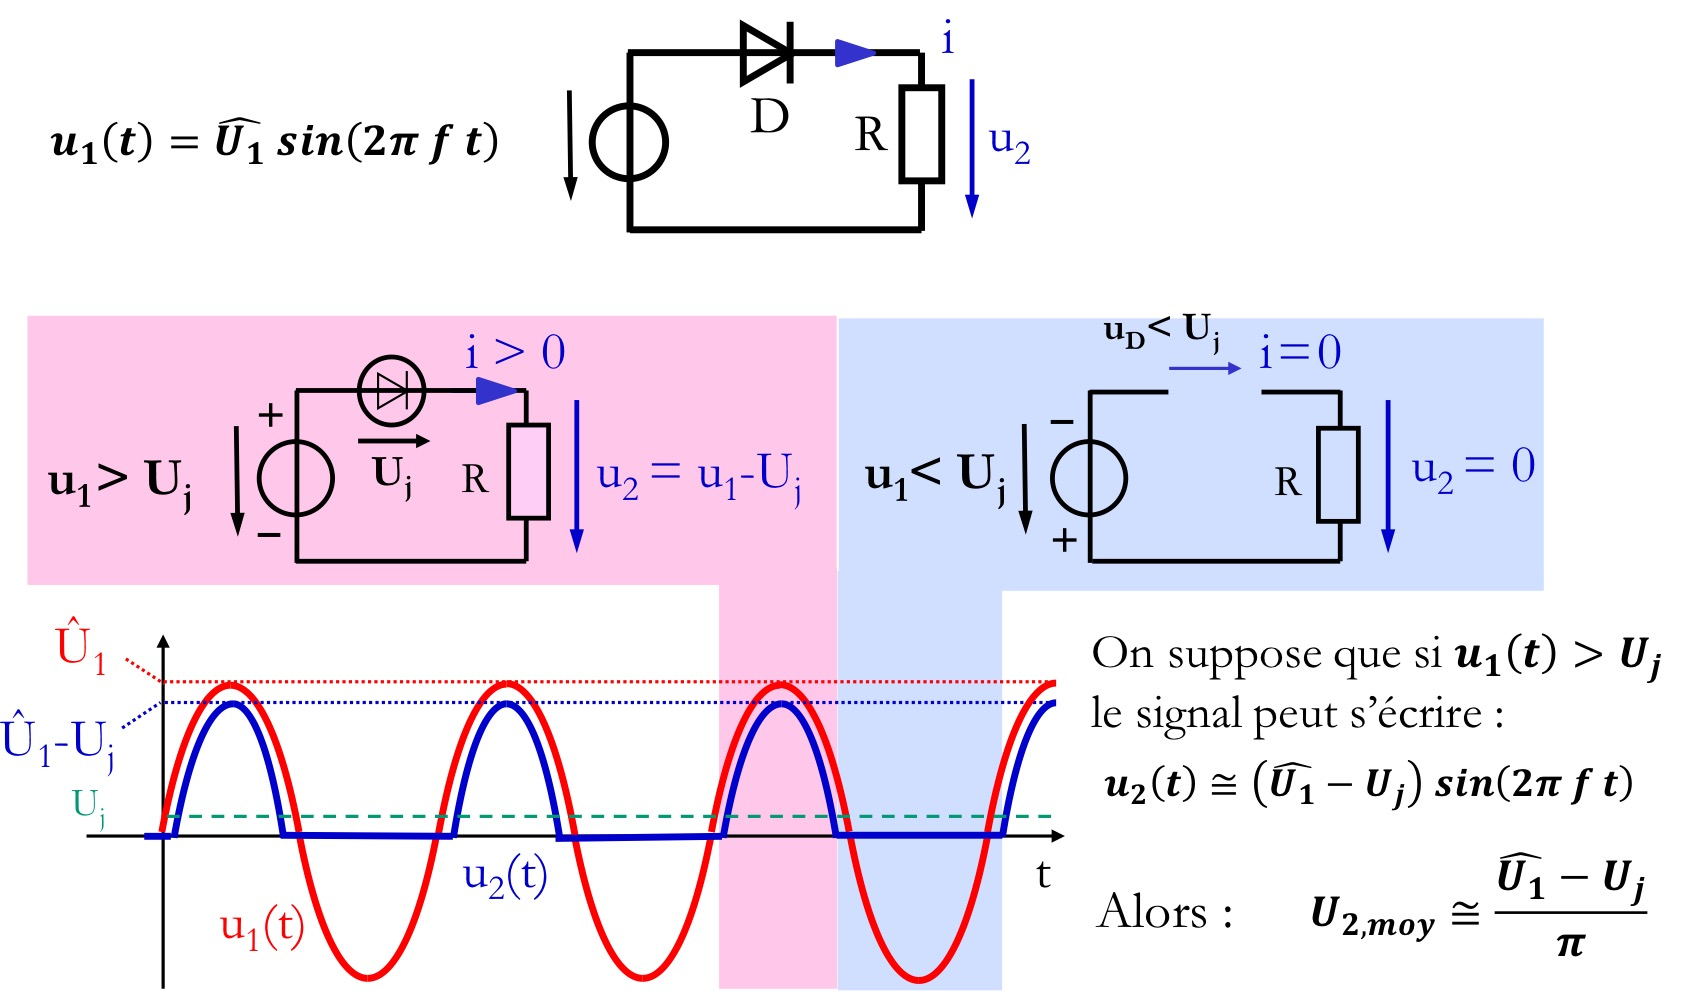
\includegraphics[width=\textwidth]{IMAGES/elec/Diode1.jpeg}
\end{figure}

\subsubsection{Redresseur double alternance en pont}
On cherche ici à prendre la valeur absolue d'un signal d'entrée.\\

\begin{figure}[hbt!]
    \centering
    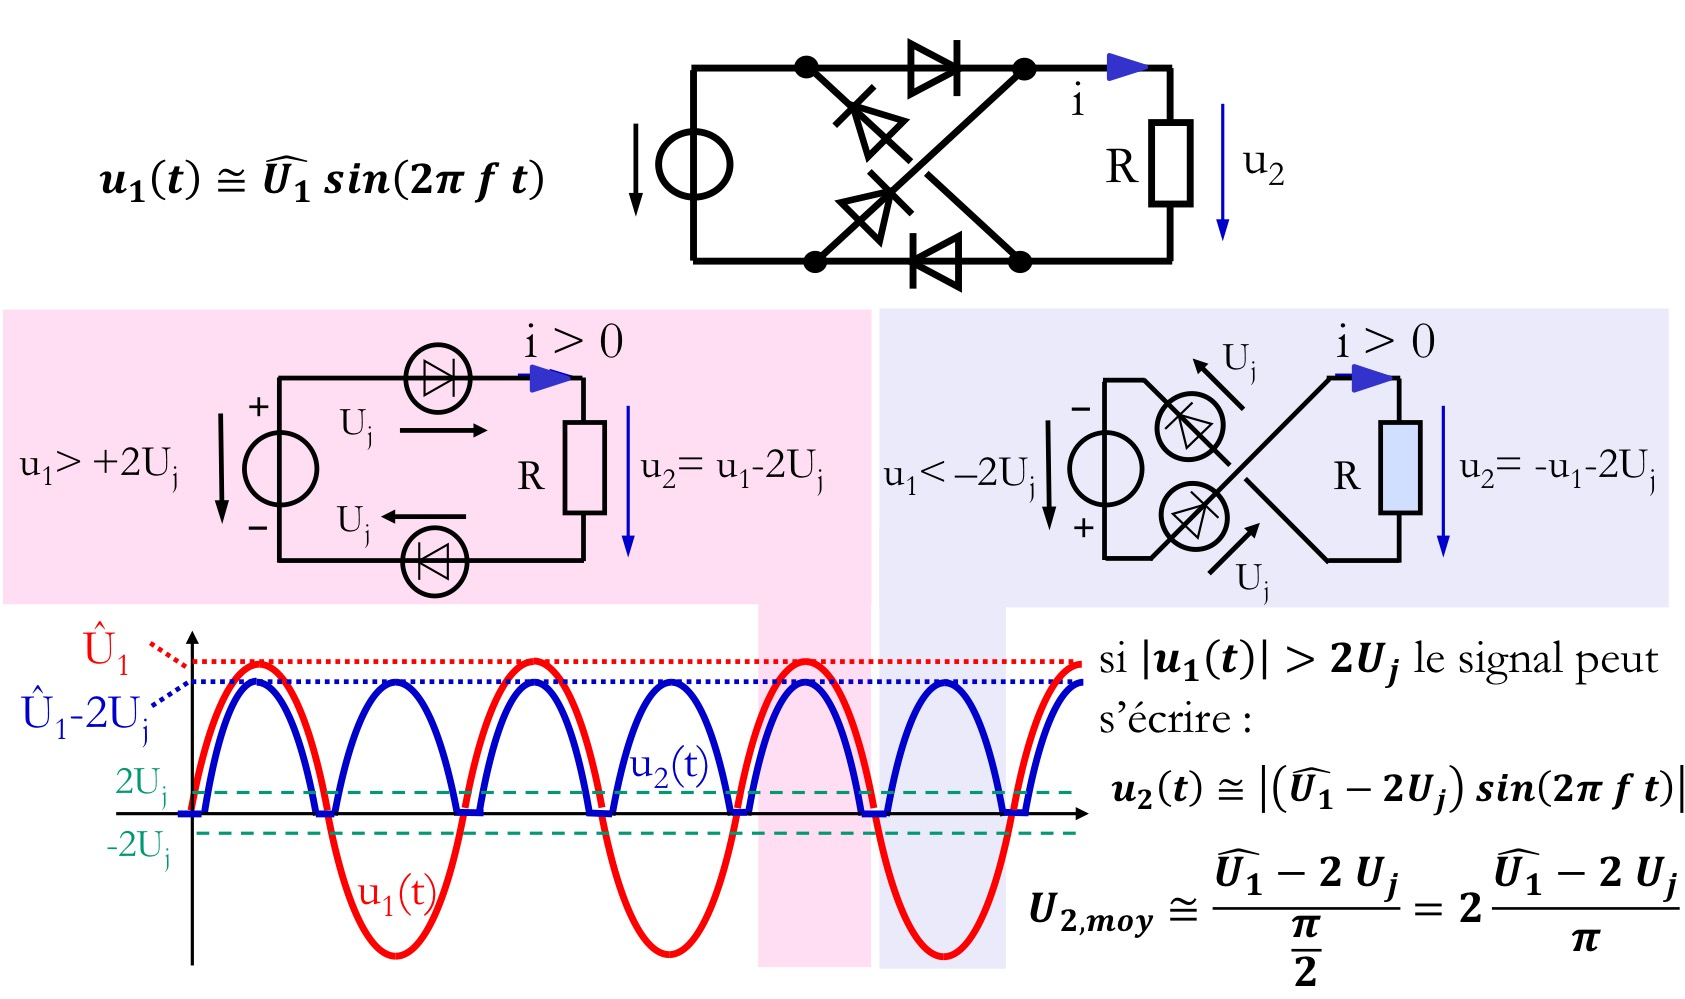
\includegraphics[width=\textwidth]{IMAGES/elec/IMG_0126.jpeg}
\end{figure}

\subsubsection{Redresseur simple alternance}
On veut transformer un signal sinusoïdale en signal continue mais avec des à-coups : \\
\begin{figure}[hbt!]
    \centering
    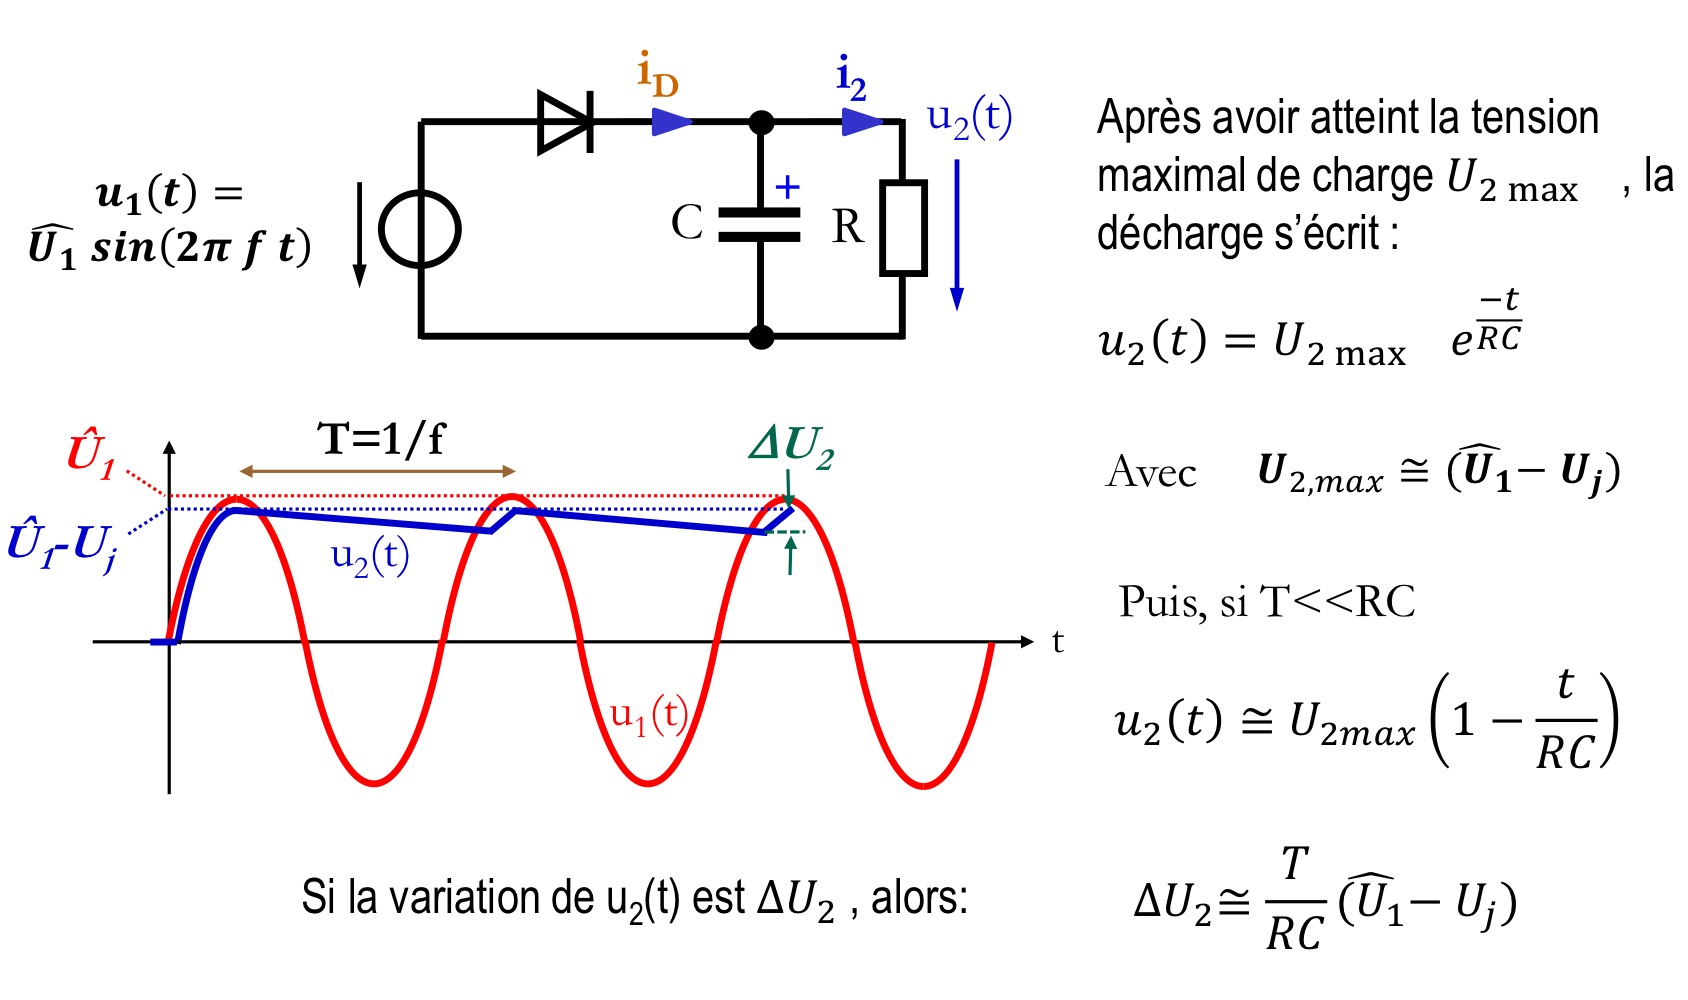
\includegraphics[width=\textwidth]{IMAGES/elec/IMG_0127.jpeg}
\end{figure}

On a ici : \begin{itemize}
    \item $U_{2,moy} = (\hat{U}_1-U_j)(1-\frac{T}{2RC})$\\
    \item $I_{2,moy} = \frac{U_{2,moy}}{R}$\\
\end{itemize}

\subsubsection{Redresseur double alternance en pont}
Il s'agit ici d'un combiné des deux autres redresseurs vu : \\

\begin{figure}[hbt!]
    \centering
    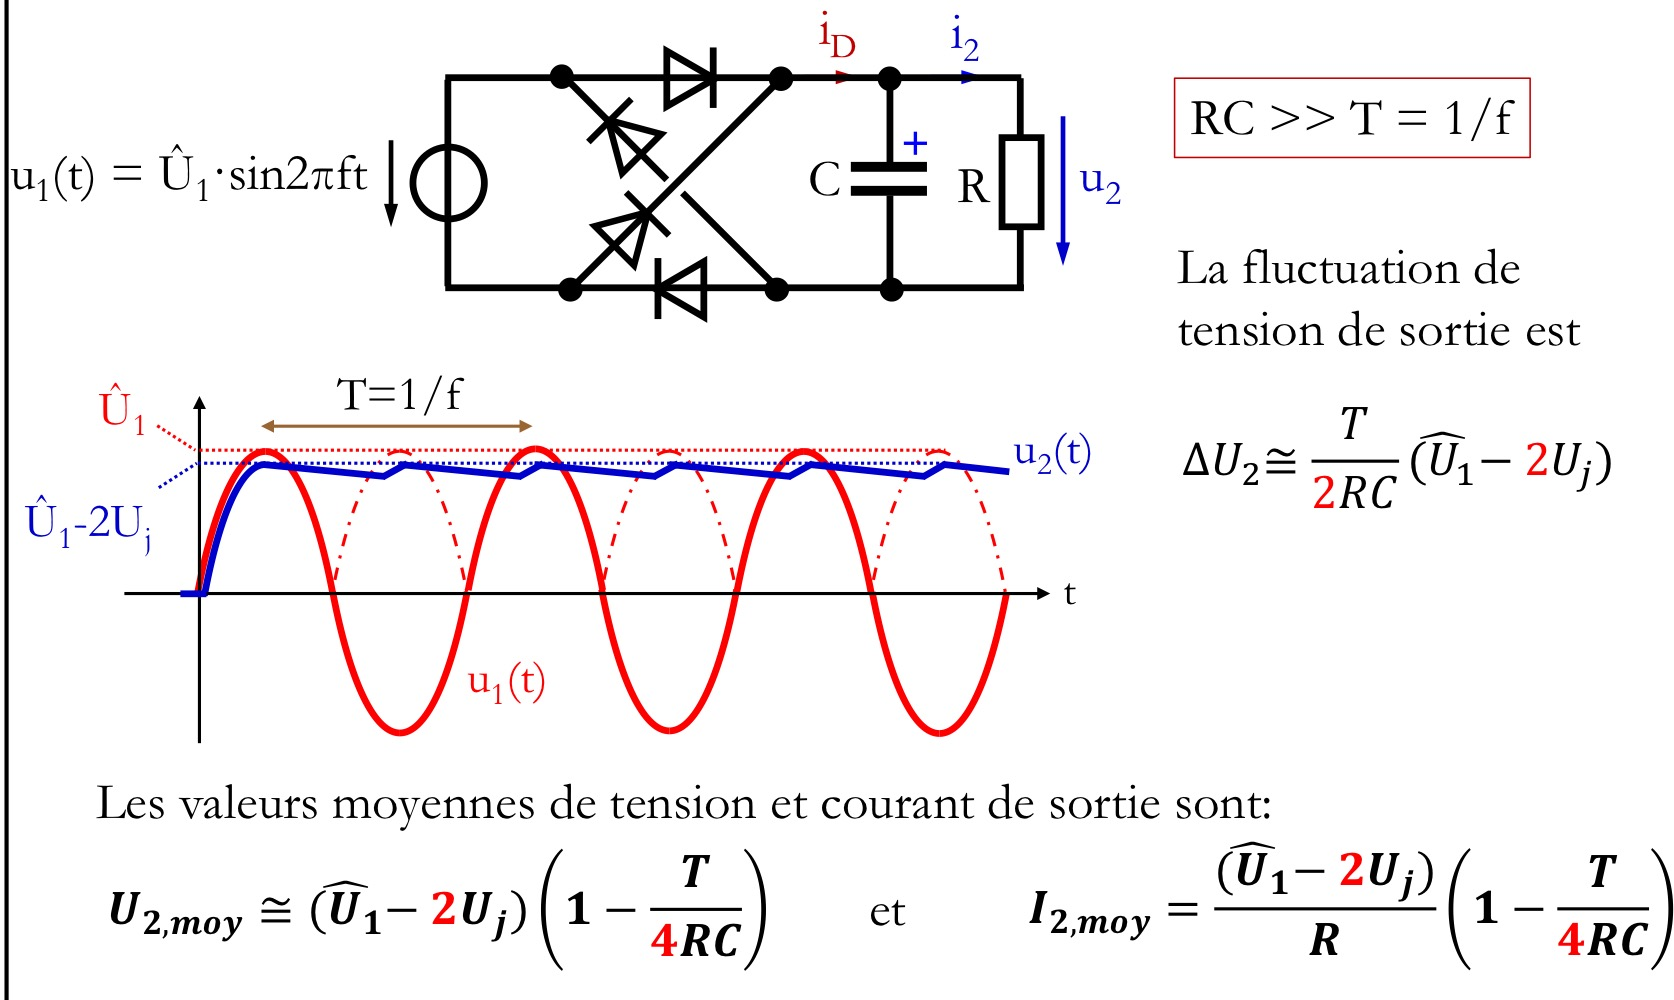
\includegraphics[width=\textwidth]{IMAGES/elec/IMG_0128.jpeg}
\end{figure}

\subsubsection{"Roue libre" : lors de commutation d'un circuit inductif}
Lors d'une coupure de courant dans un circuit LR il peut se produire des surtensions, des arcs électrique et donc endommager le système. En effet lors de la coupure, on a $\frac{di}{dt} = u_L = -\infty$\\
Pour remédier à cela, on met en parallèle une diode qui a pour but de faire baisser progressivement le courant en cas de coupure de courant.\\

\begin{figure}[hbt!]
    \centering
    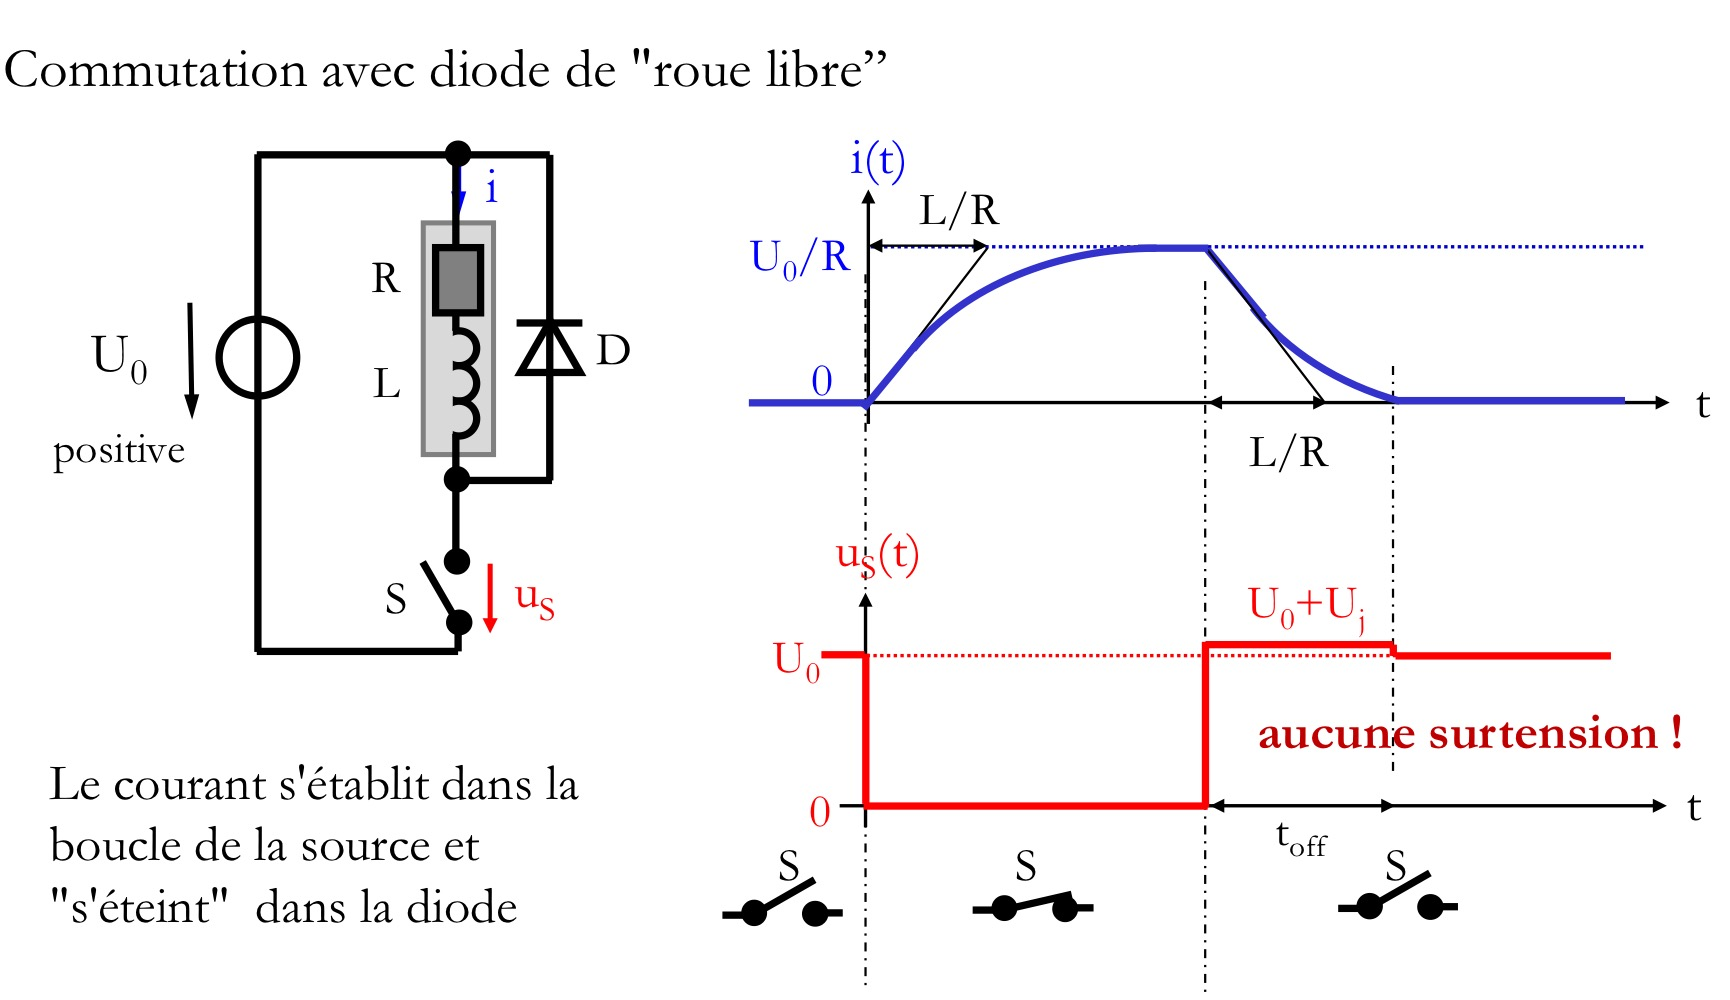
\includegraphics[width=\textwidth]{IMAGES/elec/IMG_0129.jpeg}
\end{figure}

\subsubsection{Tension de claquage}
Sous polarisation inverse, une diode est normalement bloquée. Cependant, au delà d'une tension limite $U_{BR}$ il se produit un claquage de la jonction et la diode laisse passer un courant inverse qui croit fortement pour une faible augmentation de la tension inverse.\\
$U_{BR} \simeq 10-1000$ Volts\\

\subsubsection{Diode Zener}
Les diodes Zener sont fabriquées pour présenter un claquage au-delà d'une tension donnée. Elles sont conçues pour \textbf{travailler en mode inverse} 

\subsubsection{Light Emitting Diode (LED)}
L'intensité lumineuse émise est proportionnelle au courant. La tension $U_f$ aux bornes d'une LED en mode direct est fonction des semi-conducteurs.\\
En mode inverse, la tension de claquage des LEDs est de quelques Volts seulement.\\

\subsubsection{Diode laser}
Une diode laser est une LED avec une structure et une géométrie créant une cavité résonnante optique. L'effet laser est caractérisé par une brusque augmentation de la puissance lumineuse générée qui apparaît à partir d'un courant seuil $I_T$.\\

\subsubsection{Photo-diode}
Lorsque la zone de déplétion d'une diode est illuminée, une partie de l'énergie absorbée crée des paires électron-trou libres. Elles génèrent un courant inverse qui est proportionnel au flux de photons absorbés.\\

\begin{figure}[hbt!]
    \centering
    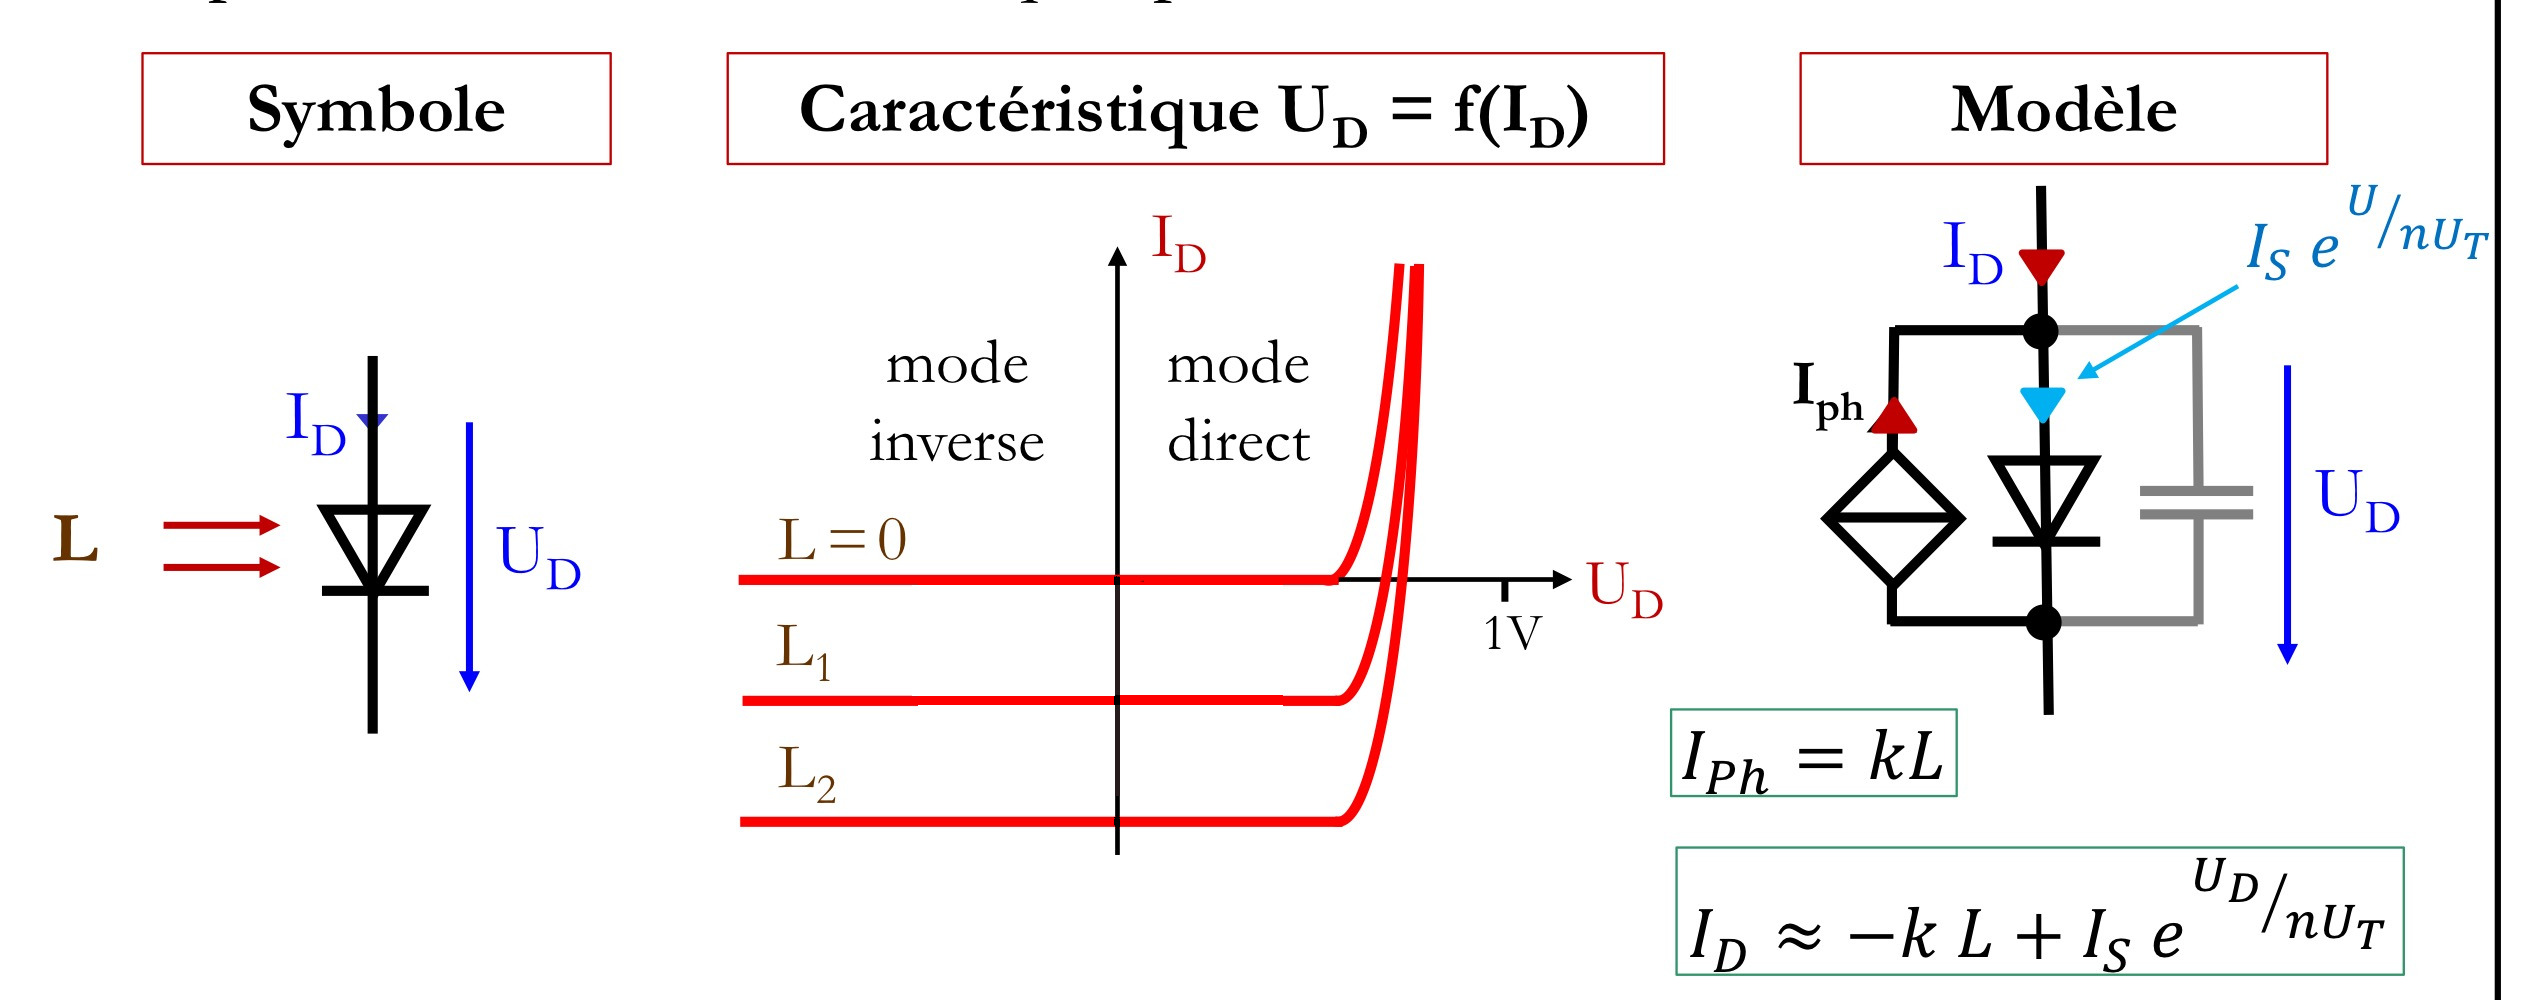
\includegraphics[width=\textwidth]{IMAGES/elec/IMG_0130.jpeg}
\end{figure}
On veut $I_D$ négatif pour récupérer l'excédent d'électrons.\\
Les panneaux solaires photo-voltaïques sont formés de photo-diodes de grande surface, assemblées en série et/ou parallèle pour obtenir une tension et courant élevés.\\

\subsection{Amplificateurs opérationnels}
Il s'agit d'un dispositif électronique à deux entrées et une sortie. Le potentiel de sortie est l'image très amplifiée de la différence de potentiel des deux entrées.\\

Il y a une saturation $V_{sat}$ au dessous de laquelle on a un profil linéaire et au dessus une constante : $v_{out} = A(v_{in+}-v_{in-}) = Au_i$\\
Avec $A>10^5$\\

Le modèle idéal est donc : \begin{itemize}
    \item un gain infini : $V_{sat-}<v_{out}<V_{sat+}$\\
    \item des courants d'entrée nuls\\
    \item une résistance de sortie nulle ($v_{out}$ indépendant de $i_{out}$)\\
\end{itemize}

\subsubsection{Réaction négative}
Le principe général de réaction négative consiste à ramener vers l'entrée une image du signal de sortie que l'on soustrait au signal initial.\\

\begin{equation}
\begin{cases}
    u_i = v_e - v_r\\
    v_r = \beta v_{out}\\
    v_{out} = Au_i\\
    \end{cases} \rightarrow v_{out} = v_e \frac{A}{1+A\beta}
\end{equation}

Si $A\rightarrow \infty \Rightarrow \begin{cases}
    v_{out} = \frac{v_e}{\beta}\\
    u_i \rightarrow 0\\
\end{cases}$\\

Un amplificateur avec un très grand gain va donc ajuster sa sortie de façon à égaliser le potentiel d'entrée $v_e$ avec le potentiel de la réaction $v_f$ et va adopter un comportement qui ne dépend que de la réaction $\beta$.\\

\subsubsection{Amplificateur opérationnel proportionnel non inverseur}

\begin{figure}[hbt!]
    \centering
    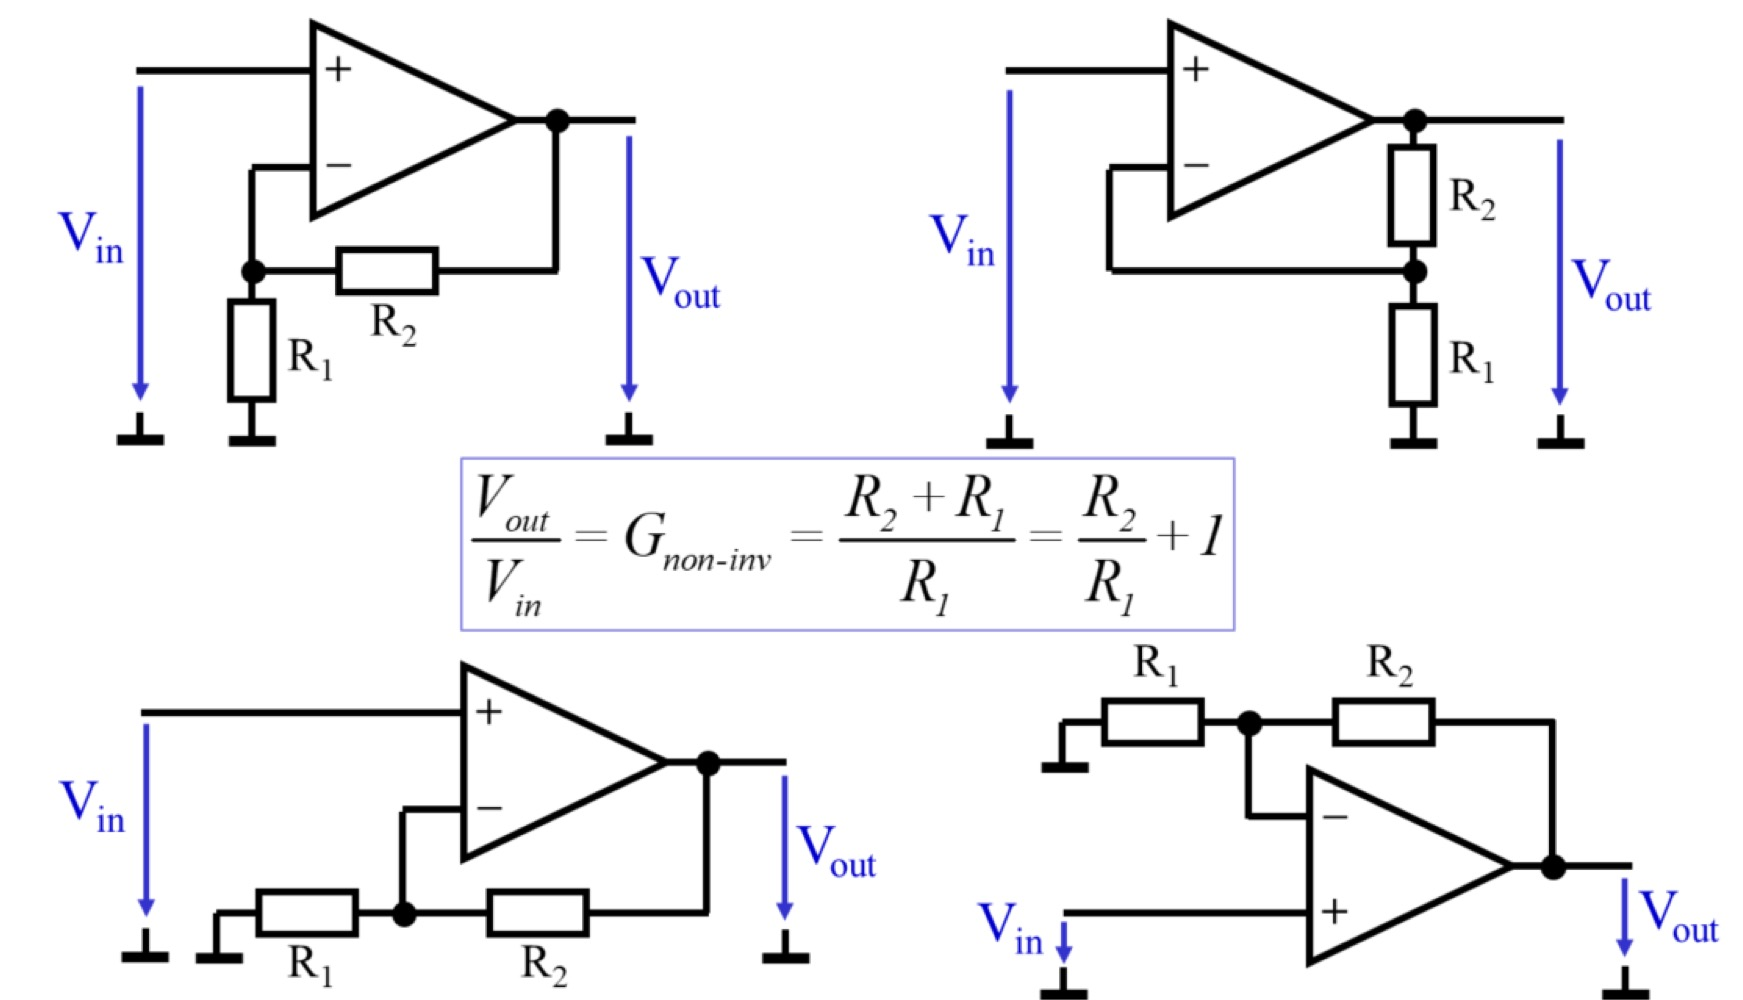
\includegraphics[width = .7\textwidth]{IMAGES/elec/IMG_0131.jpeg}
\end{figure}

\begin{equation}
    \beta = \frac{R_1}{R_1+R_2}
\end{equation}


\subsubsection{Amplificateur inverseur}

\begin{figure}[hbt!]
    \centering
    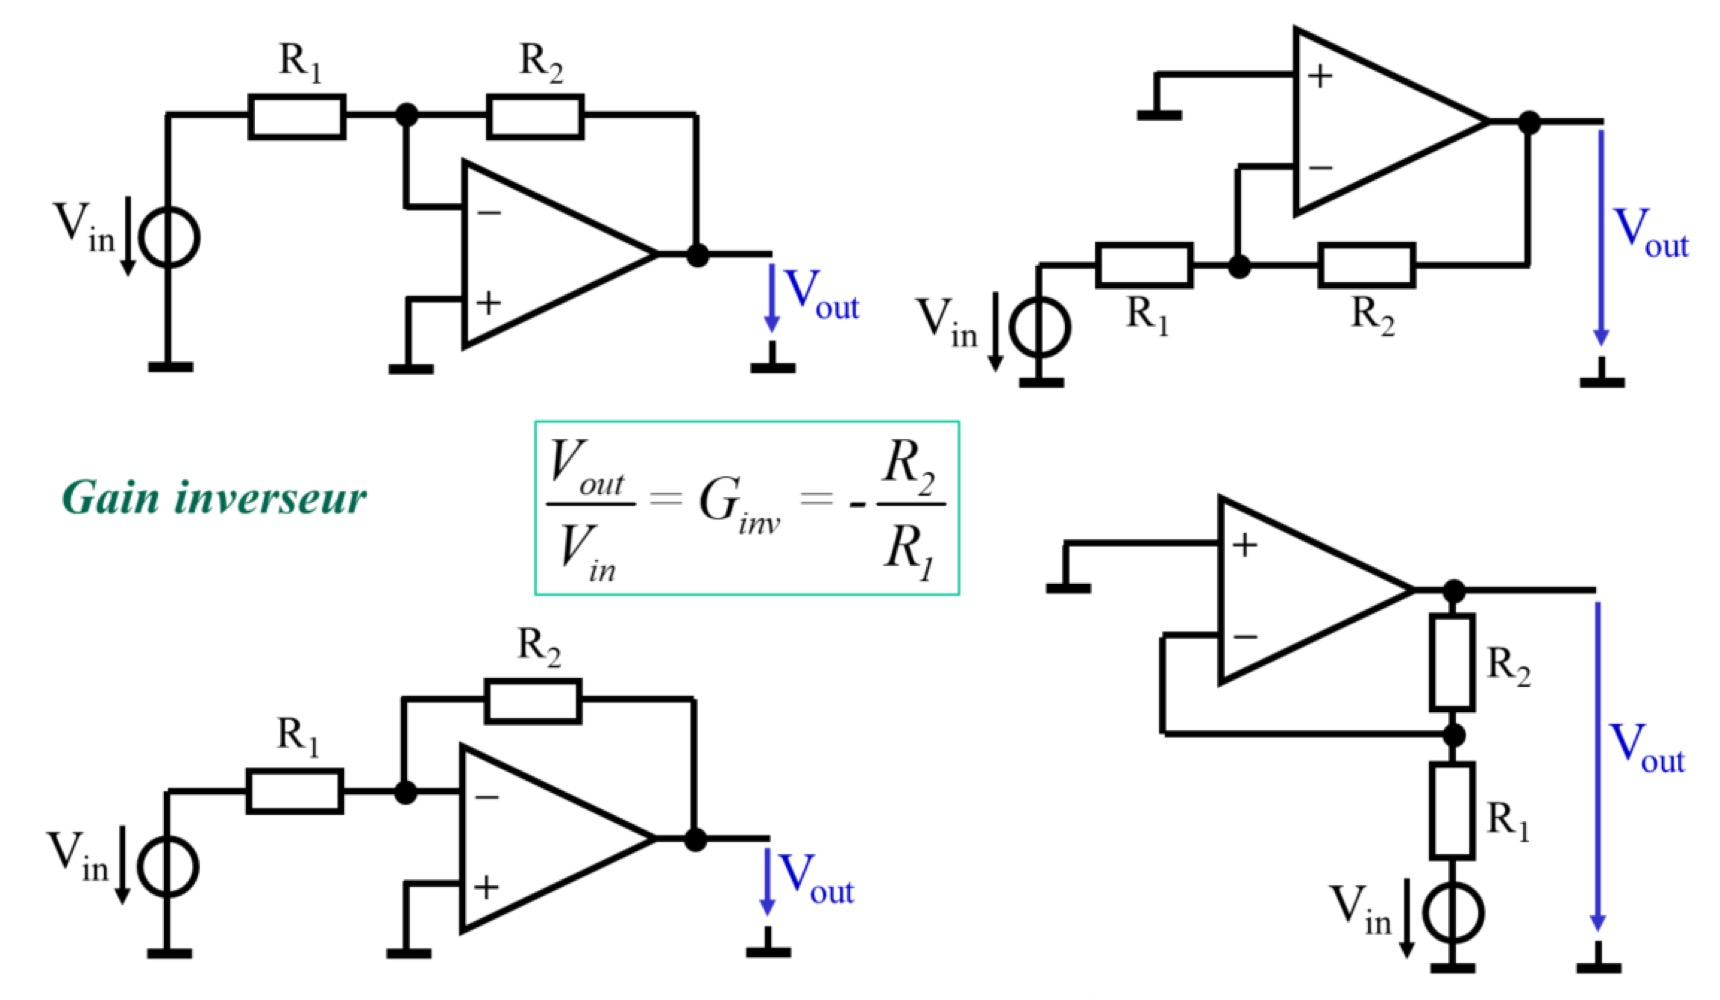
\includegraphics[width=.7\textwidth]{IMAGES/elec/IMG_0132.jpeg}
\end{figure}

\begin{equation}
    \beta = -\frac{R_2}{R_1}
\end{equation}

Le noeud A est à un potentiel nul mais aucun courant ne circule de ce point vers la masse : c'est une \textbf{masse fictive}.\\

\subsubsection{Intégrateur inverseur}

\begin{figure}[hbt!]
    \centering
    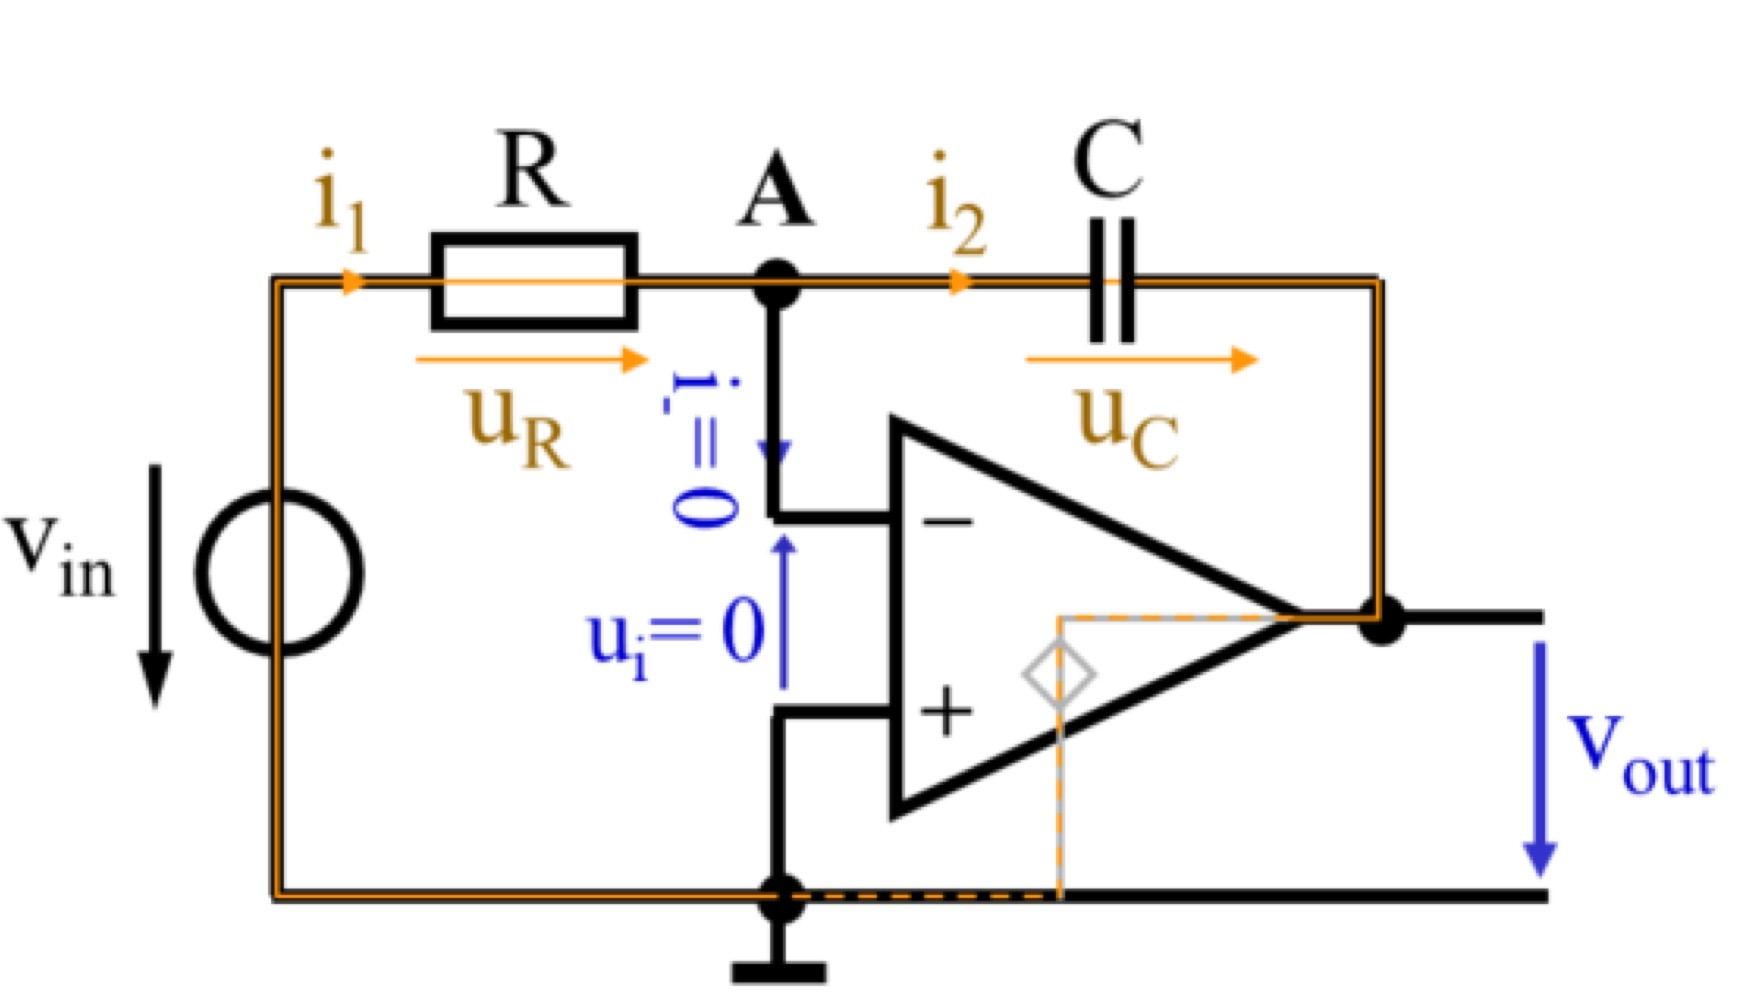
\includegraphics[width=.7\textwidth]{IMAGES/elec/IMG_0133.jpeg}
\end{figure}

\begin{equation}
    V_{out} = V_{out}(0) - \frac{1}{RC} \int V_{in}dt
\end{equation}

En régime sinus : $H(j\omega) = \frac{V_{out}}{V_{in}} = -\frac{1}{j\omega RC}$\\

\subsubsection{Dérivateur inverseur}

\begin{figure}[hbt!]
    \centering
    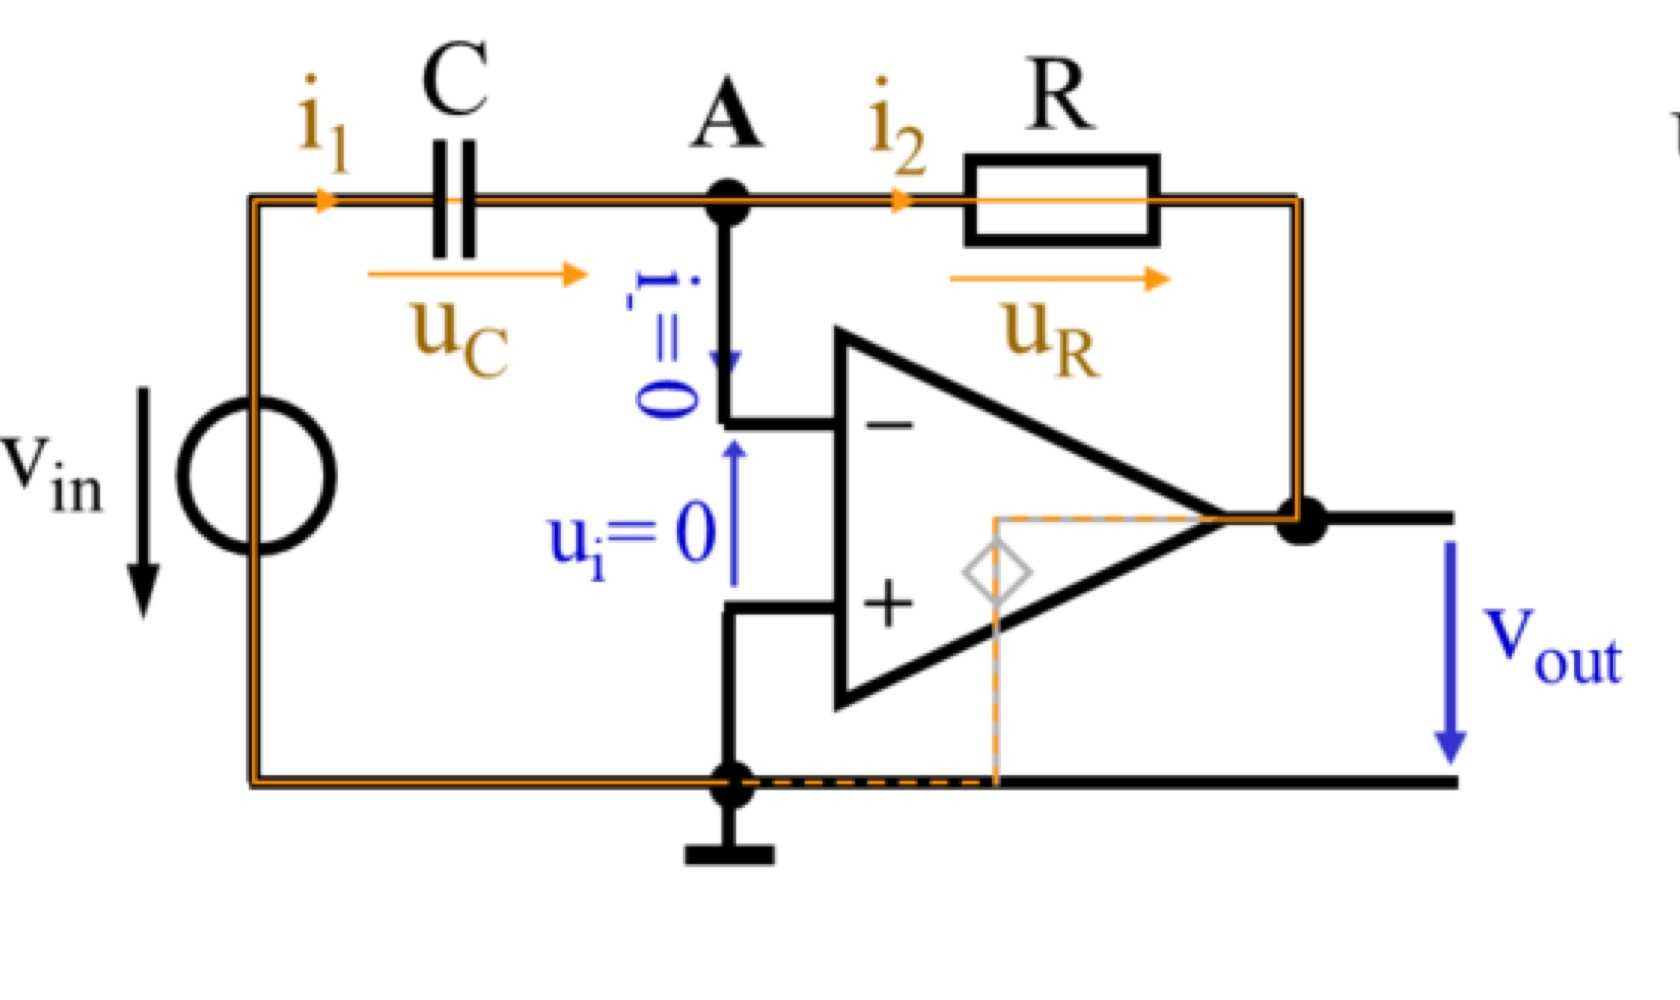
\includegraphics[width=.7\textwidth]{IMAGES/elec/IMG_0134.jpeg}
\end{figure}

\begin{equation}
    V_{out} = -RC \frac{dV_{in}}{dt}
\end{equation}

En régime sinus : $H(j\omega) = -\omega RC$\\

\subsubsection{Sommateur inverseur}

On peut sommer plusieurs signaux ensemble : \\

\begin{figure}[hbt!]
    \centering
    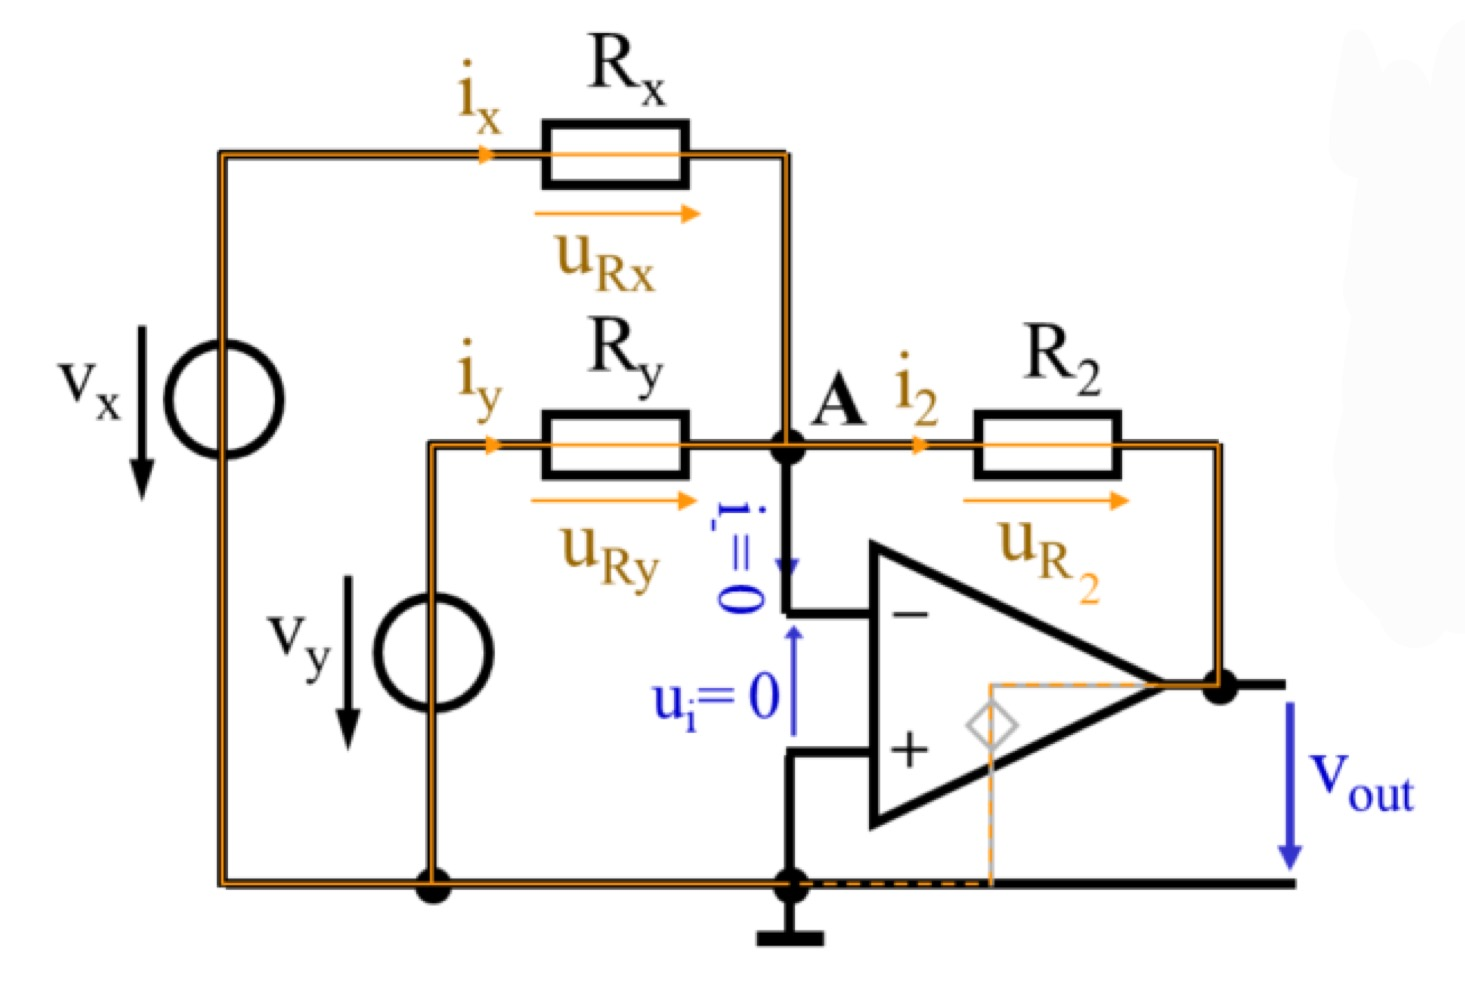
\includegraphics[width=.7\textwidth]{IMAGES/elec/IMG_0135.jpeg}
\end{figure}

On a ici : $V_{out} = -\frac{R_2}{R_x}v_x - \frac{R_2}{R_y}v_y$\\


Grâce à ces amplificateurs opérationnels inverseur sommateur, on peut réaliser un régulateur PID.\\

\subsubsection{Filtrage basses-fréquences}
Pour éviter les signaux parasites et ne laisser passer que les fréquences en dessous d'une valeur limite $f_p$.\\
\textbf{On ajoute une capacité C en parallèle avec R}.\\

\subsubsection{Comparateur}

En l'absence de réaction négative, sa sortie peut être considérée comme binaire : $V_{sat+}$ ou $V_{sat-}$\\

L'amplificateur opérationnel fonctionne ici en comparateur simple.\\
La sortie d'un comparateur sature à deux valeurs $V_{OH}$ et $V_{OL}$.\\

\begin{figure}[hbt!]
    \centering
    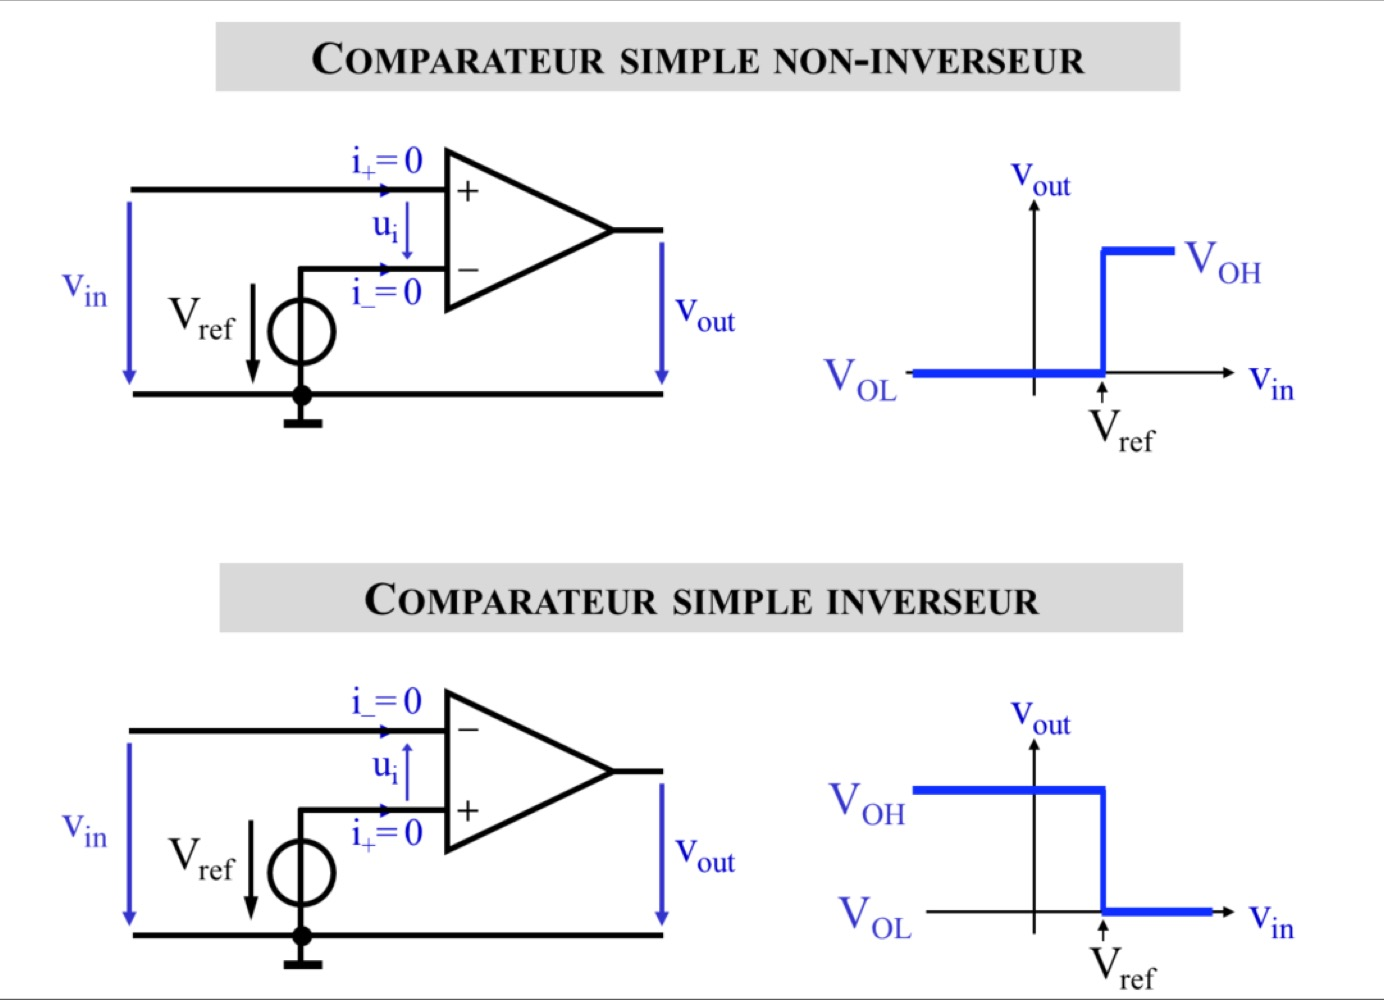
\includegraphics[width=.6\textwidth]{IMAGES/elec/IMG_0137.jpeg}
\end{figure}

\subsubsection{Redresseur idéal}

\begin{figure}[hbt!]
    \centering
    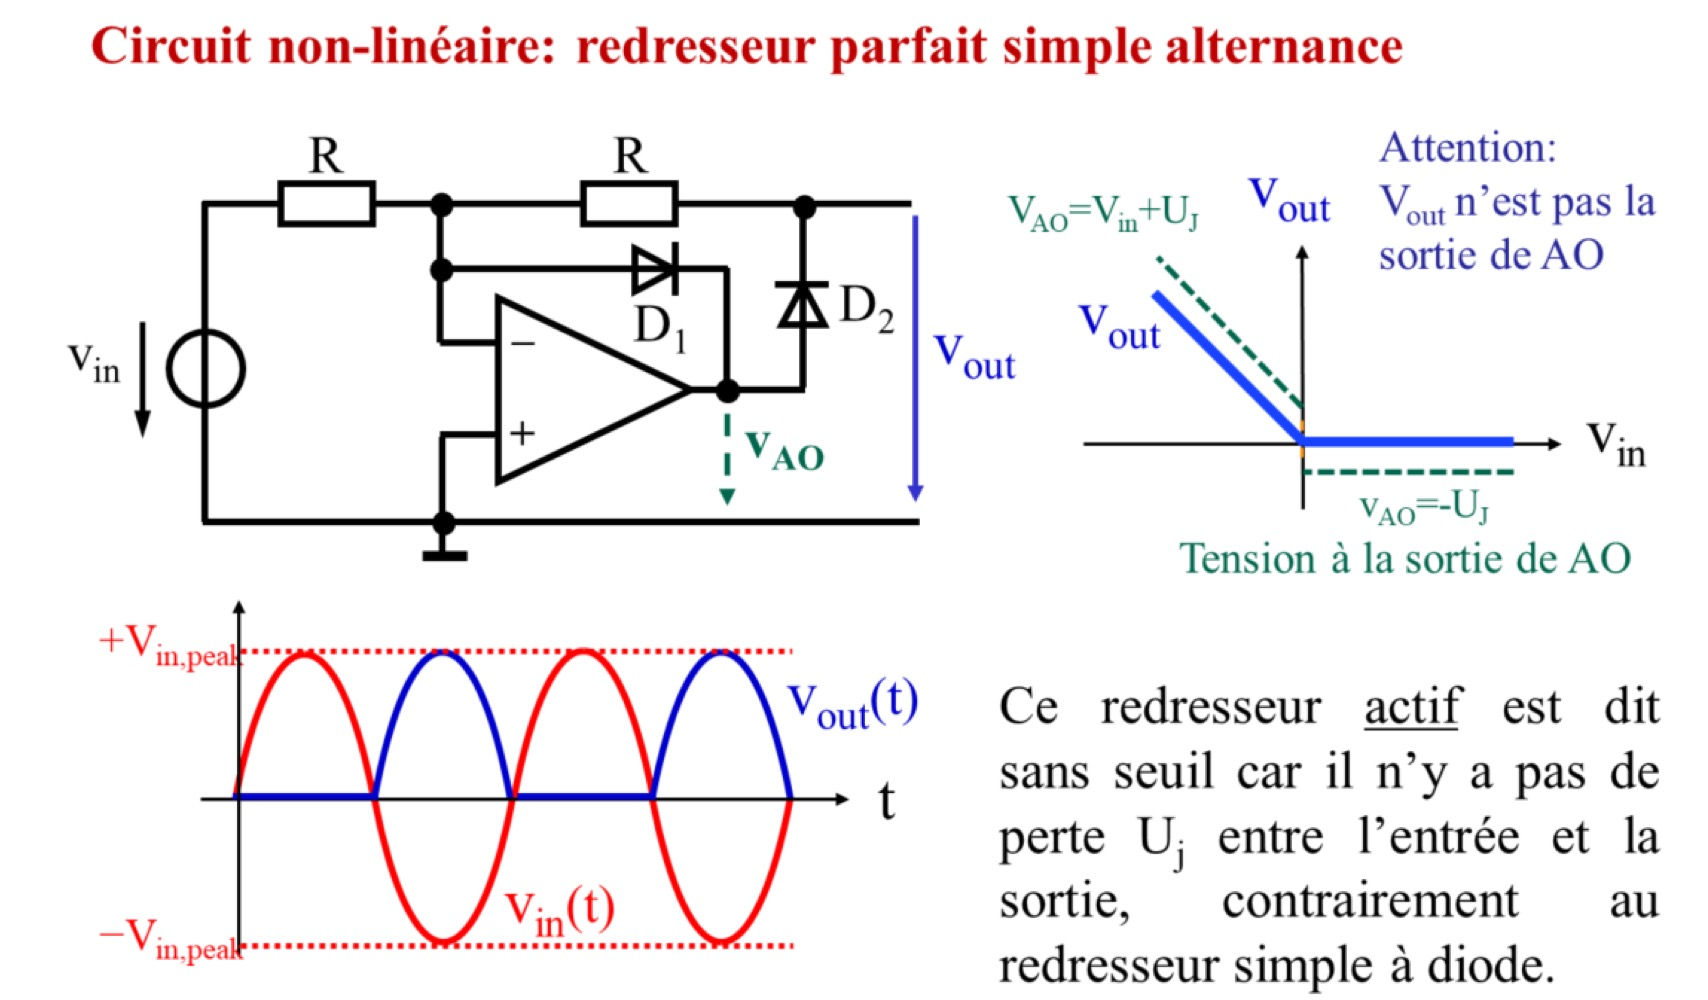
\includegraphics[width=.6\textwidth]{IMAGES/elec/IMG_0138.jpeg}
\end{figure}

\begin{figure}[hbt!]
    \centering
    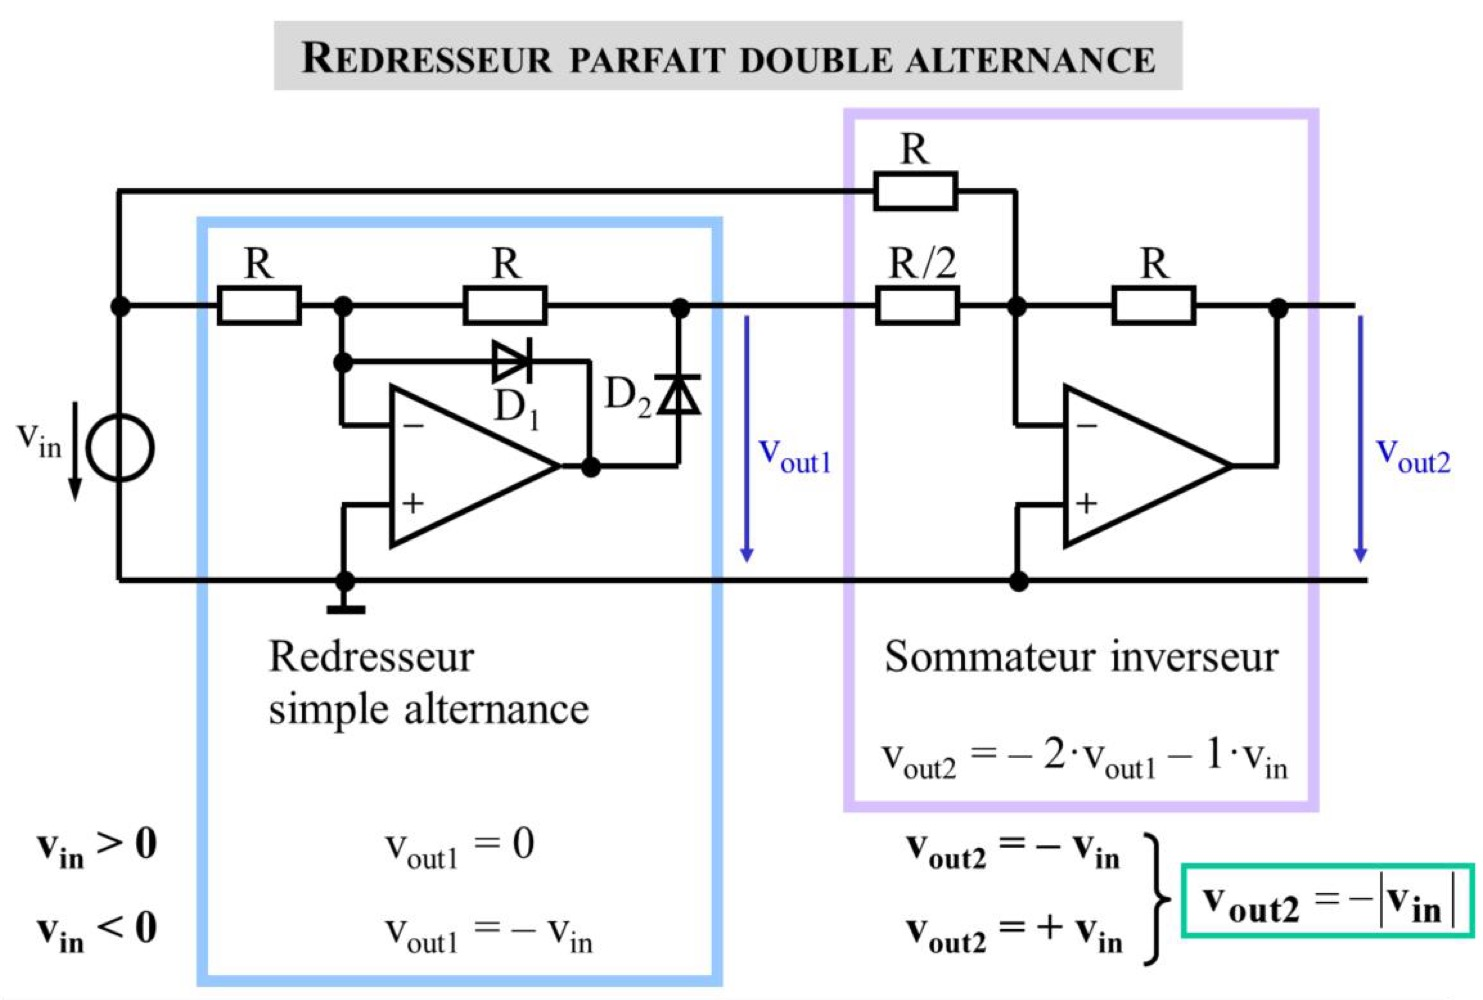
\includegraphics[width=.6\textwidth]{IMAGES/elec/IMG_0139.jpeg}
\end{figure}

Ici, $v_{out} = - \lvert v_{in}\rvert$.\\

\subsubsection{L'amplificateur différentiel}
La tension de sortie ne déprend que de la différence de tension entre ses deux entrées. \begin{equation}
    v_{out} = A_{diff} (v_1-v_2) = A_{diff} u_{in,diff}
\end{equation}
Avec $A_{diff}$ : le gain différentiel\\

\begin{figure}[hbt!]
    \centering
    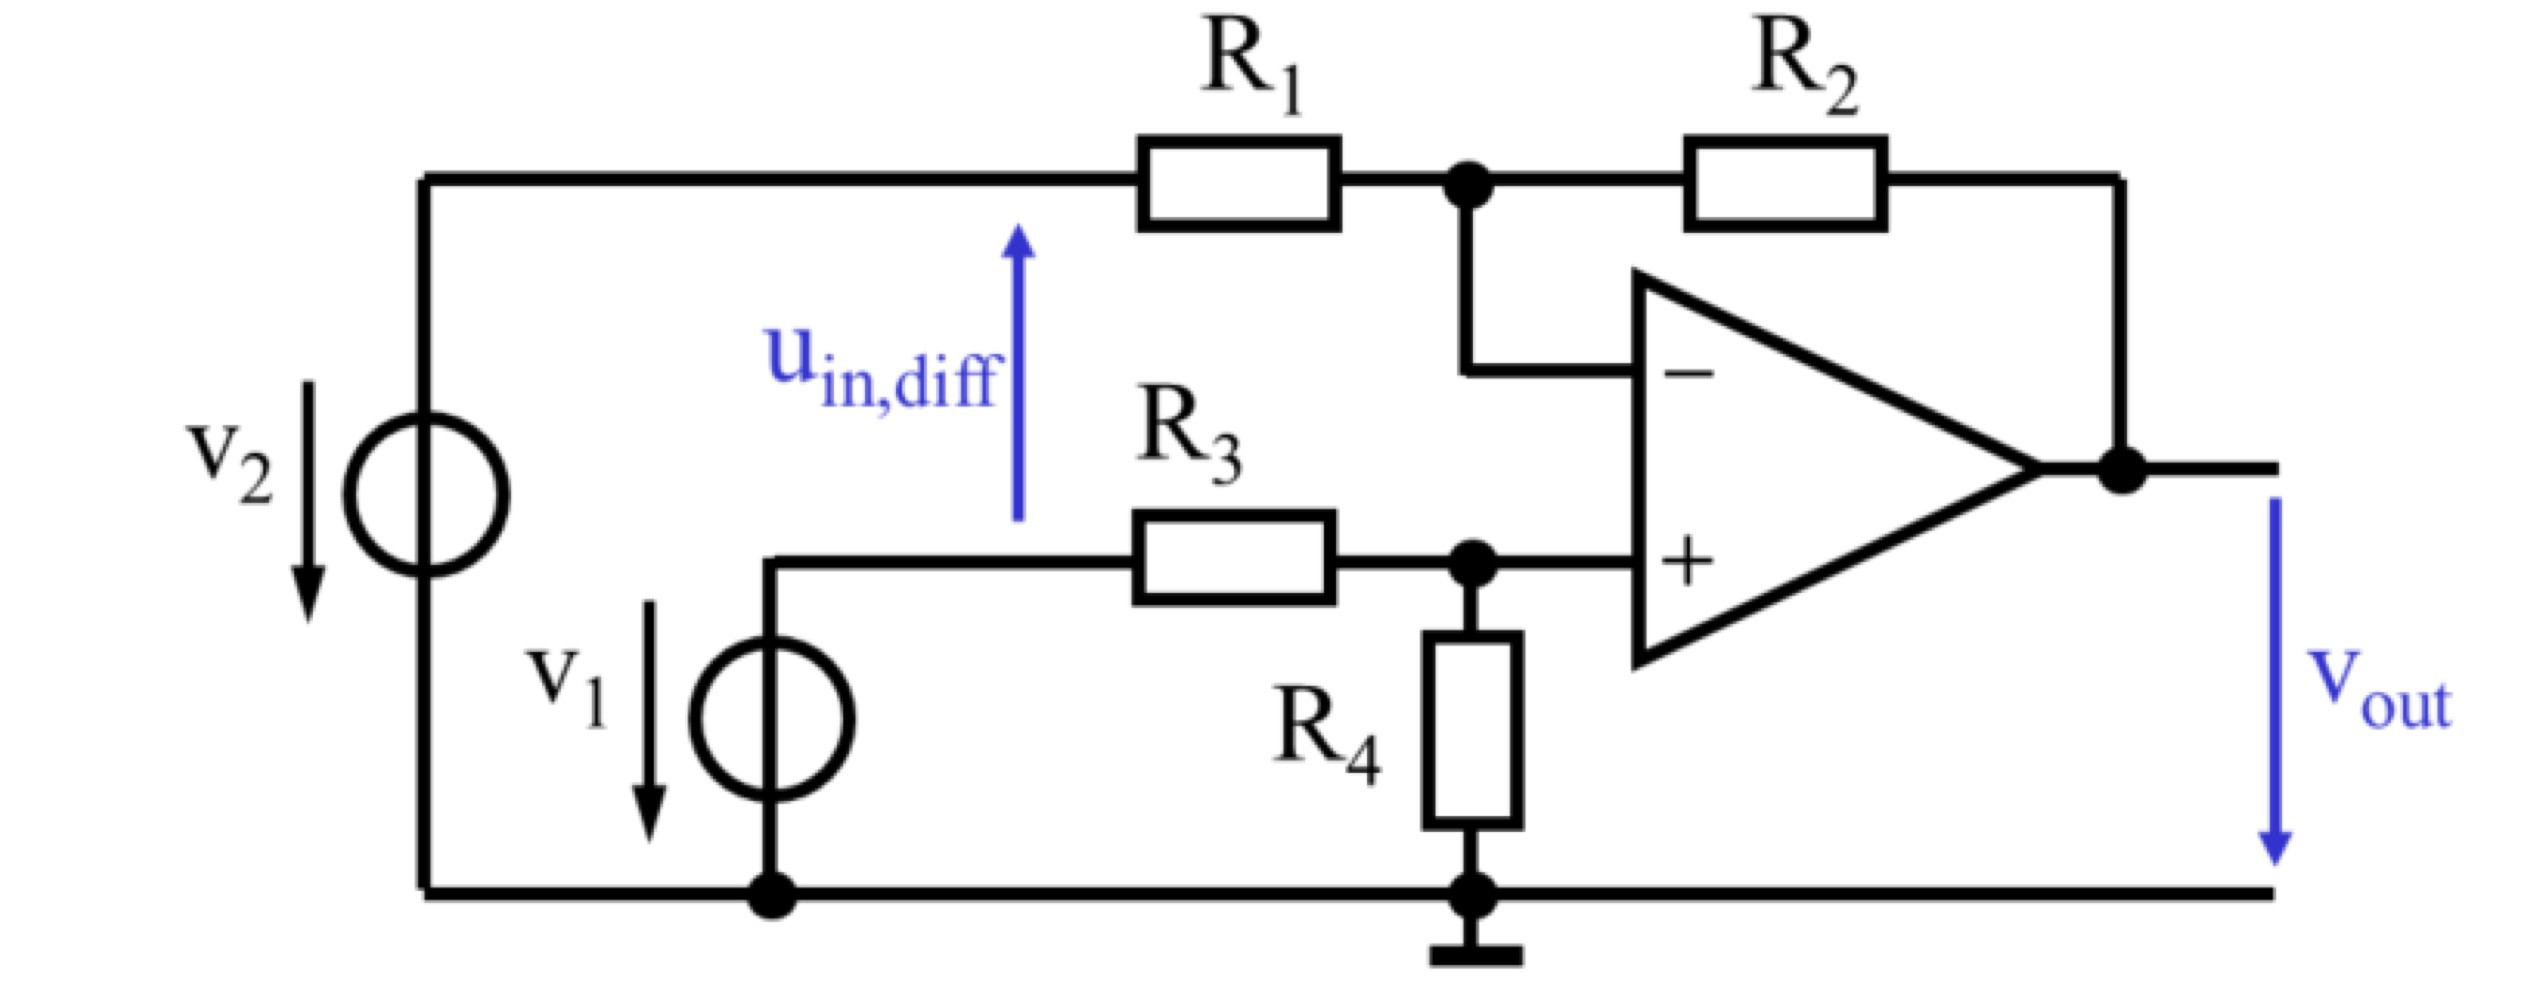
\includegraphics[width=.6\textwidth]{IMAGES/elec/IMG_0140.jpeg}
\end{figure}

On a : \begin{equation}
    v_{out} = \frac{R_2+R_1}{R_1} \frac{R_4}{R_4+R_3} v_1 - \frac{R_2}{R_1}v_2
\end{equation}

Si on a un ampli purement différentiel alors : $\frac{R_2+R_1}{R_1} \frac{R_4}{R_4+R_3} \Rightarrow \frac{R_2}{R_1} = \frac{R_4}{R_3} = A_{diff}$\\

\quad \underline{Mode commun :}\\

Ce mode est donnée par $\frac{v_1+v_2}{2}$, on peut alors définir le gain en ode commun : \begin{equation}
    A_{mc} = \frac{v_{out}}{u_{in-mc}}
\end{equation}
où $v_1=v_2= u_{in-mc}$\\

\textbf{Le taux de réjection en mode commun CMRR} : CMRR = $\frac{A_{diff}}{A_{mc}}$\\

\warning Plus le CMRR est élevé, meilleur est l'amplificateur différentiel.\\

Il existe deux inconvénients à cette approche : \begin{itemize}
    \item Un courant circule à travers les sources $V_1$ et $V_2$, ce qui pourrait changer les valeurs si leur impédance internes sont élevées (capteurs). Les tensions mesurées sont alors $V_{1ext}$ et $V_{2ext}$\\
    \item On doit changer simultanément deux résistances pour changer le gain\\
\end{itemize}

\quad \underline{Amplificateur différentiel hautes performances :}\\

On peut s'affranchir de l'impédance élevée des capteurs en introduisant 2 suiveurs de tension. Le courant dans les capteurs sera nul et les tensions appliquées aux bornes de l'amplificateur différentiel seront les tensions non-perturbées.\\

\begin{figure}[hbt!]
    \centering
    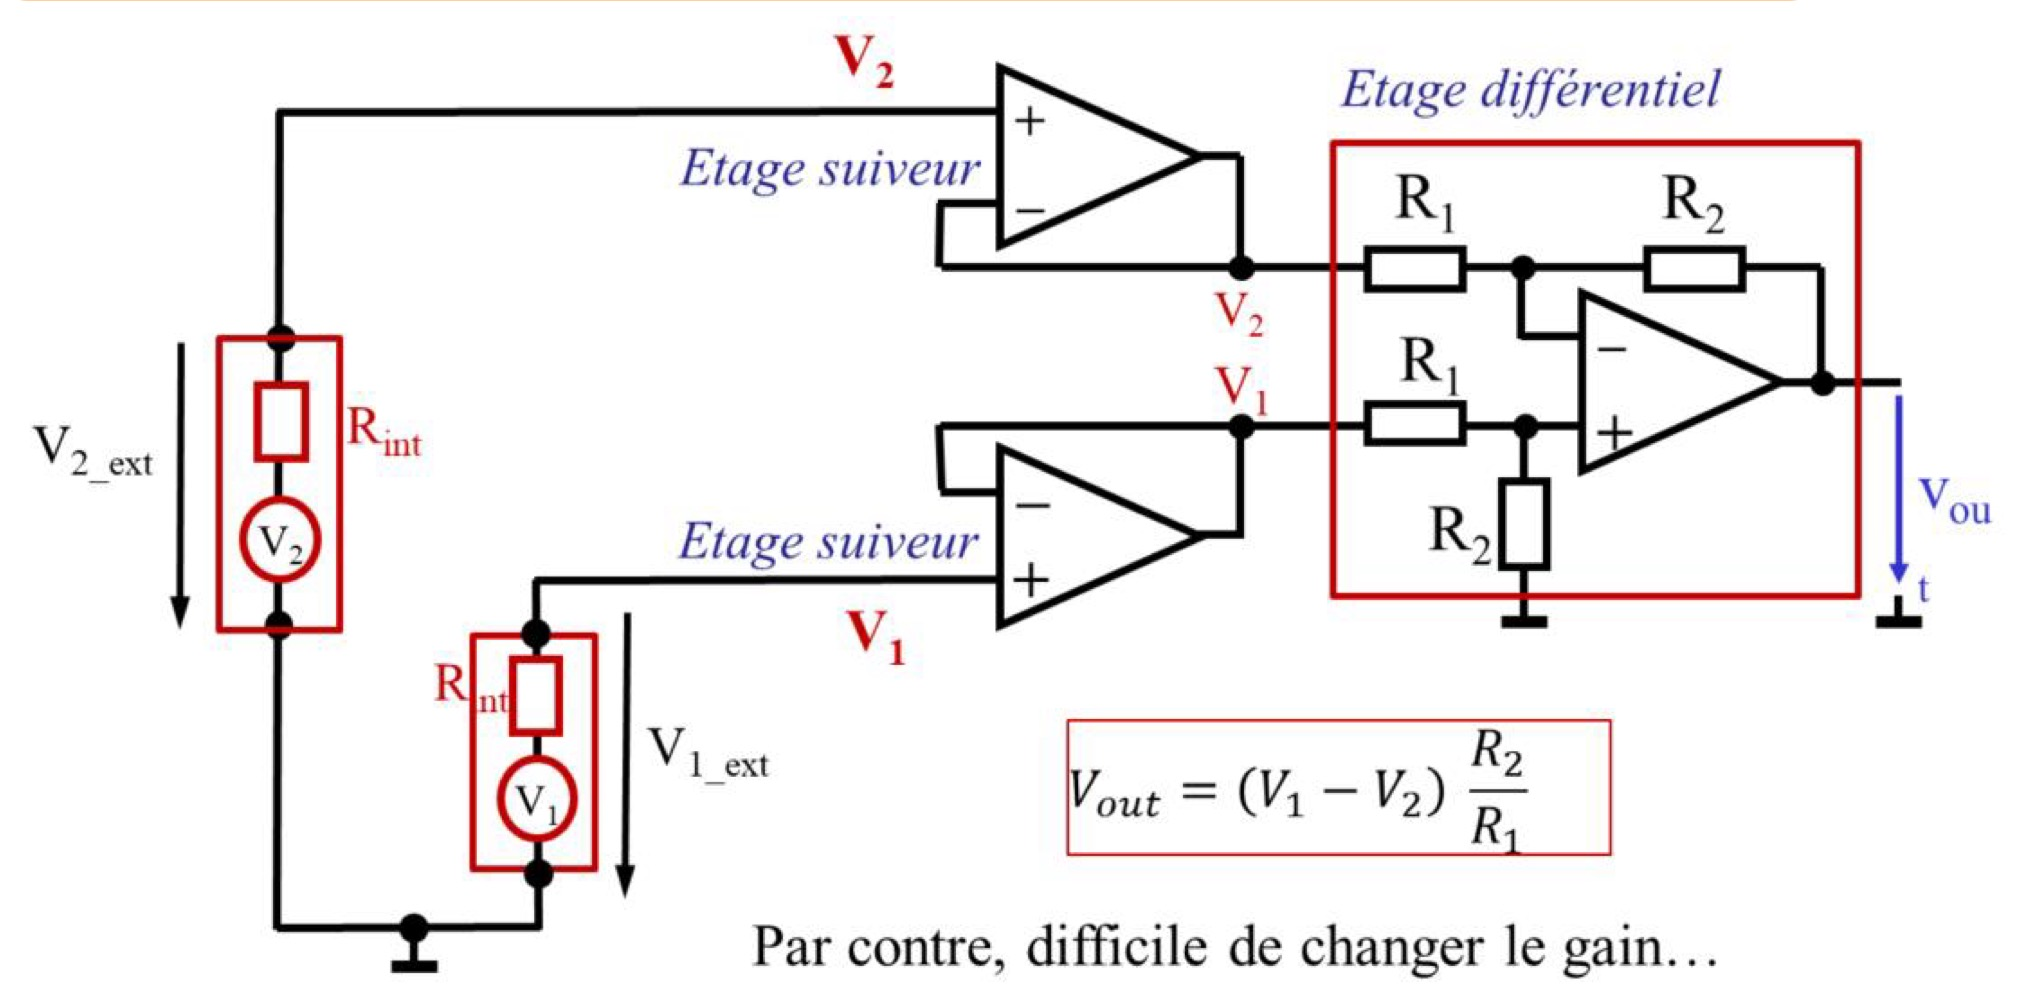
\includegraphics[width=.6\textwidth]{IMAGES/elec/IMG_0141.jpeg}
\end{figure}

On peut également réaliser un étage différentiel où le gain peut être changé via $R_4$.\\

\begin{figure}[hbt!]
    \centering
    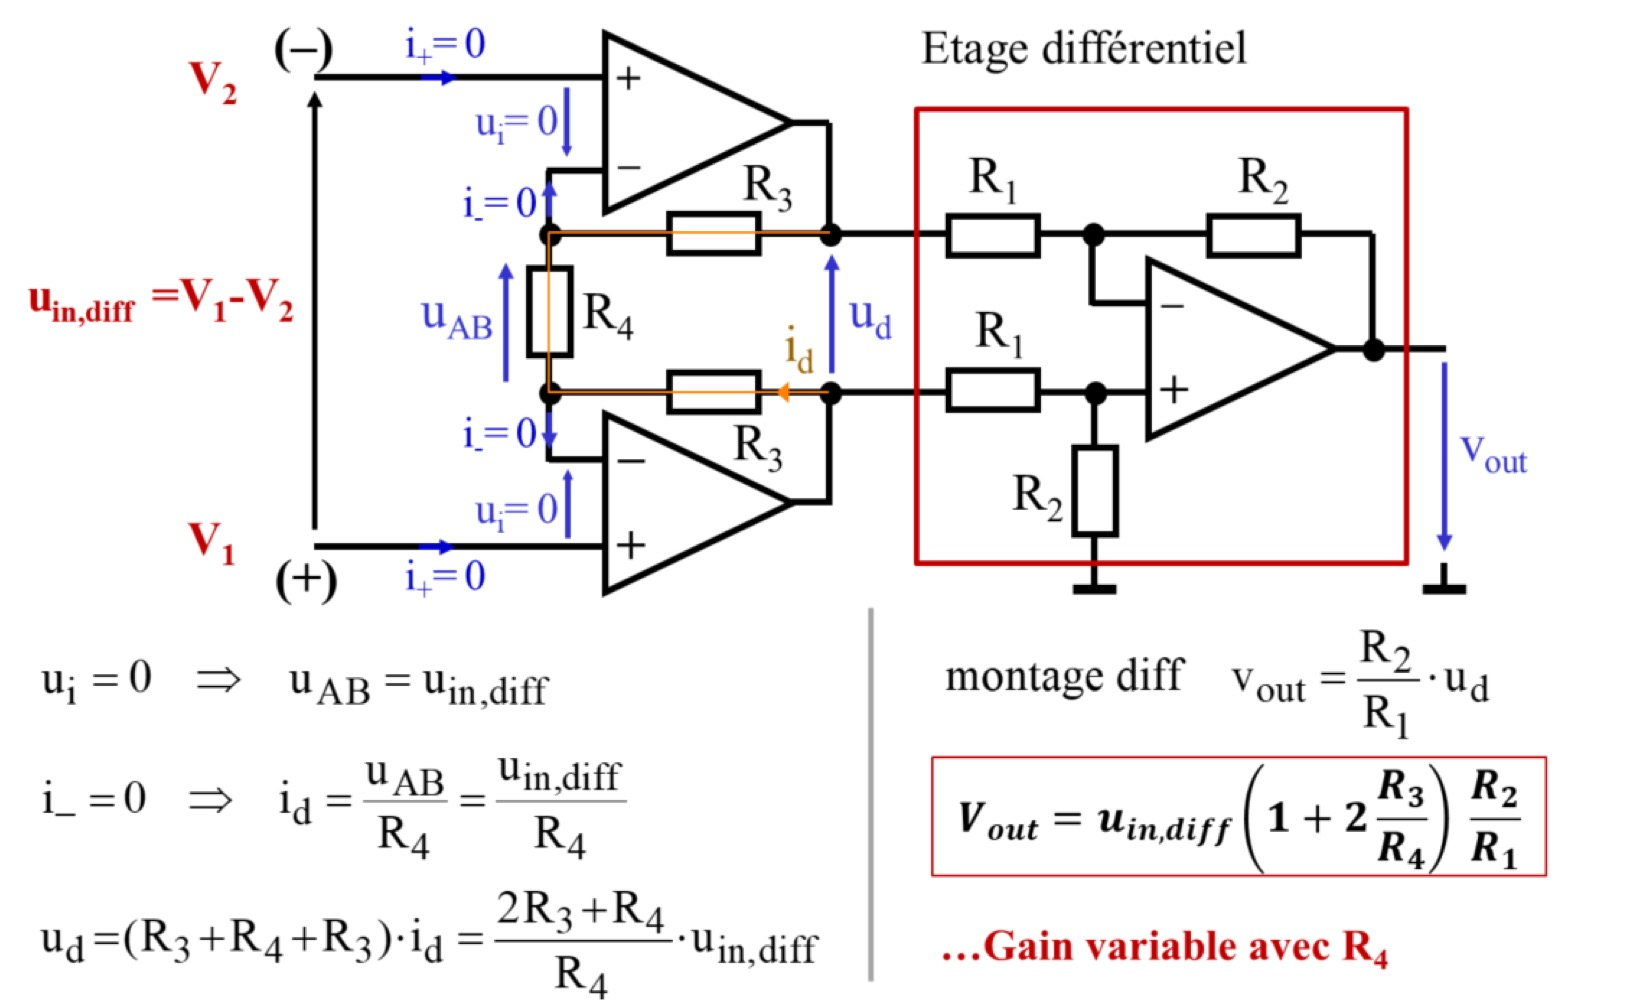
\includegraphics[width=.6\textwidth]{IMAGES/elec/IMG_0142.jpeg}
\end{figure}

On a également la variante à deux ampli op. : \\

\begin{figure}[hbt!]
    \centering
    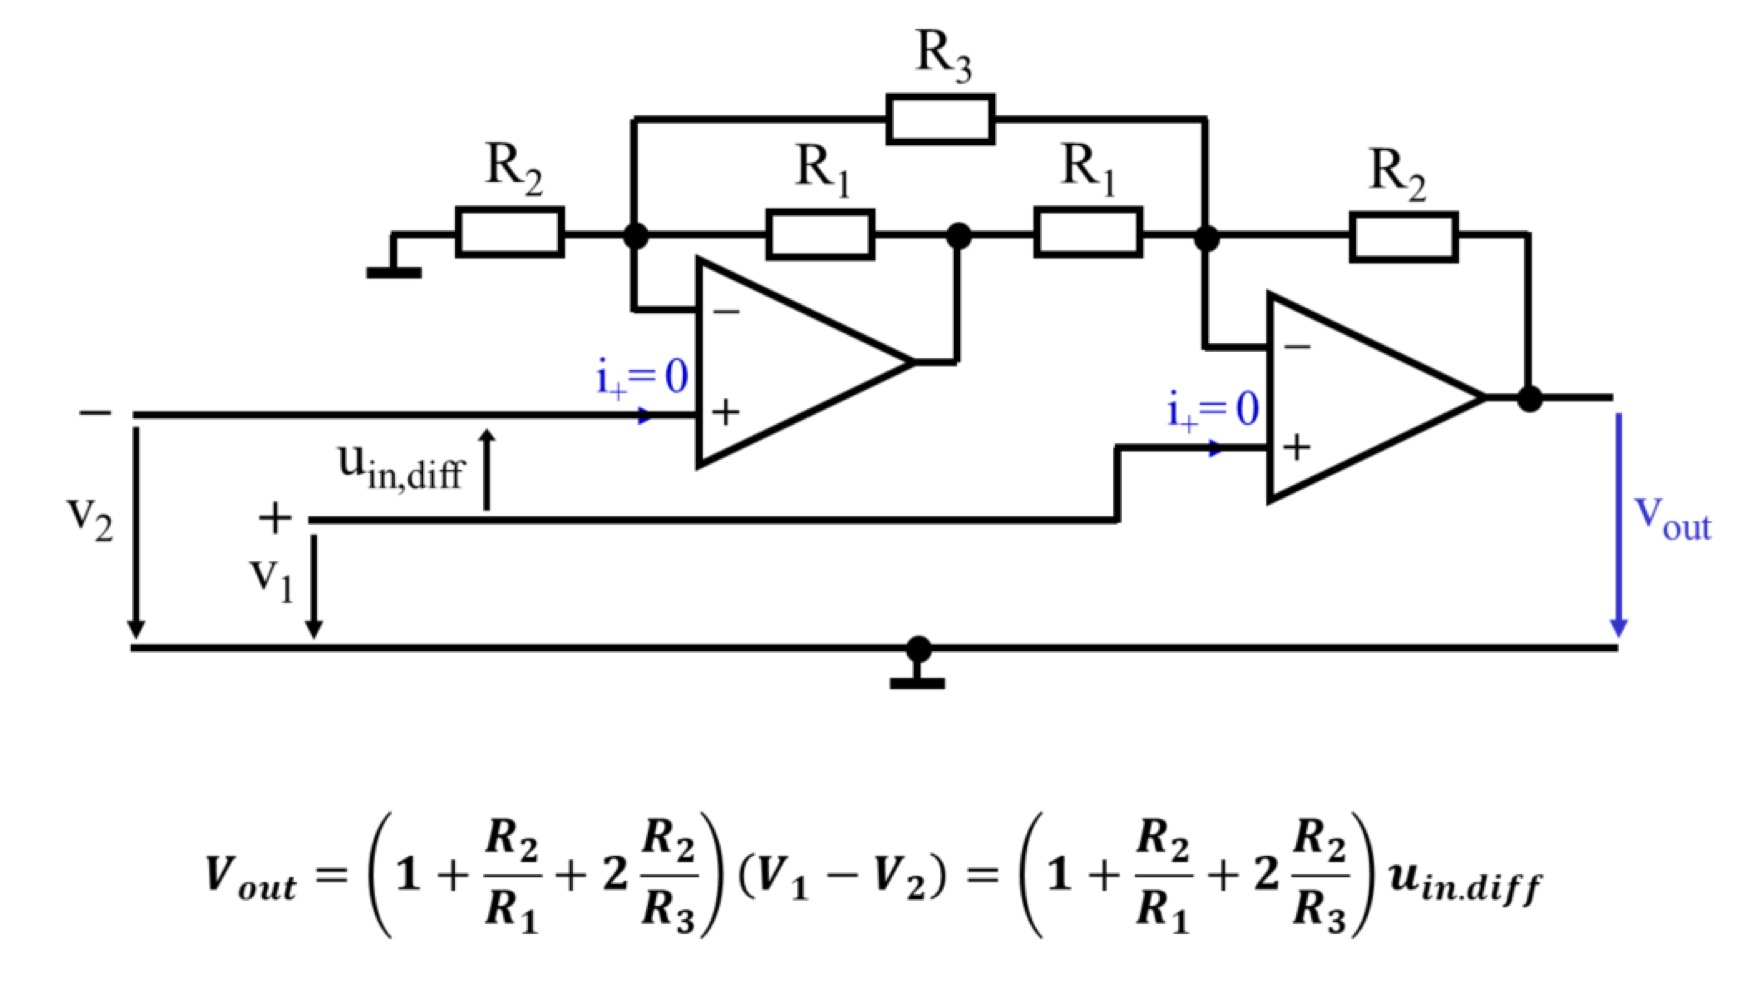
\includegraphics[width=.6\textwidth]{IMAGES/elec/IMG_0143.jpeg}
\end{figure}

\subsubsection{L'AO en réaction positive}

La réaction consiste ici à ramener une image du signal de sortie pour l'additionner au signal initial d'entrée.\\

\begin{itemize}
    \item la sortie ne peut prendre que deux valeurs $V_{sat+} = V_{OH}$ ou $V_{sat-} = V_{OL}$\\
    \item la sortie change d'état lorsque $u_i$ change de signe, donc passe par zéro.\\
\end{itemize}

\warning Il n'y a pas d'état d'équilibre stable.\\

La sortie change donc d'état si $u_i$ change de signe donc dès que $v_+ = v_-$.\\
Dans le cas où la source $v_2$ est reliée à la résistance $R_1$ et à la borne positive de l'AO et la source $v_1$ est reliée à la borne négative de l'AO, on a : \\
\begin{equation}
\begin{gathered}
    \frac{R_2}{R_1+R_2} v_2 + \frac{R_1}{R_1+R_2}V_{OH} = v_1\\
    \frac{R_2}{R_1+R_2} v_2 + \frac{R_1}{R_1+R_2}V_{OL} = v_1\\
    \end{gathered}
\end{equation}

On trouve une hystérèse dans ce cas. En effet, la sortie descend de $V_{OH}$ à $V_{OL}$ à partir d'une certaine valeur $V_{T1}$. De même, elle monte entre ces deux valeurs à partir de $V_{T2}$. La différence entre les deux vaut donc : \begin{equation}
    \Delta V_T = V_{T1}-V_{T2}
\end{equation}

Deux cas sont possibles : \begin{itemize}
    \item la source $v_2$ est à une référence fixe alors que $v_1$ varie. On trouve : \begin{equation}
         \Delta V_T= \frac{R_1}{R_1+R_2} (V_{OH}-V_{OL})
    \end{equation}
    \item la source $v_2$ varie alors que $v_1$ est à une référence : \begin{equation}
        \Delta V_T = \frac{R_1}{R_2} (V_{OH}-V_{OL})
    \end{equation}
\end{itemize}

\begin{figure}[hbt!]
    \centering
    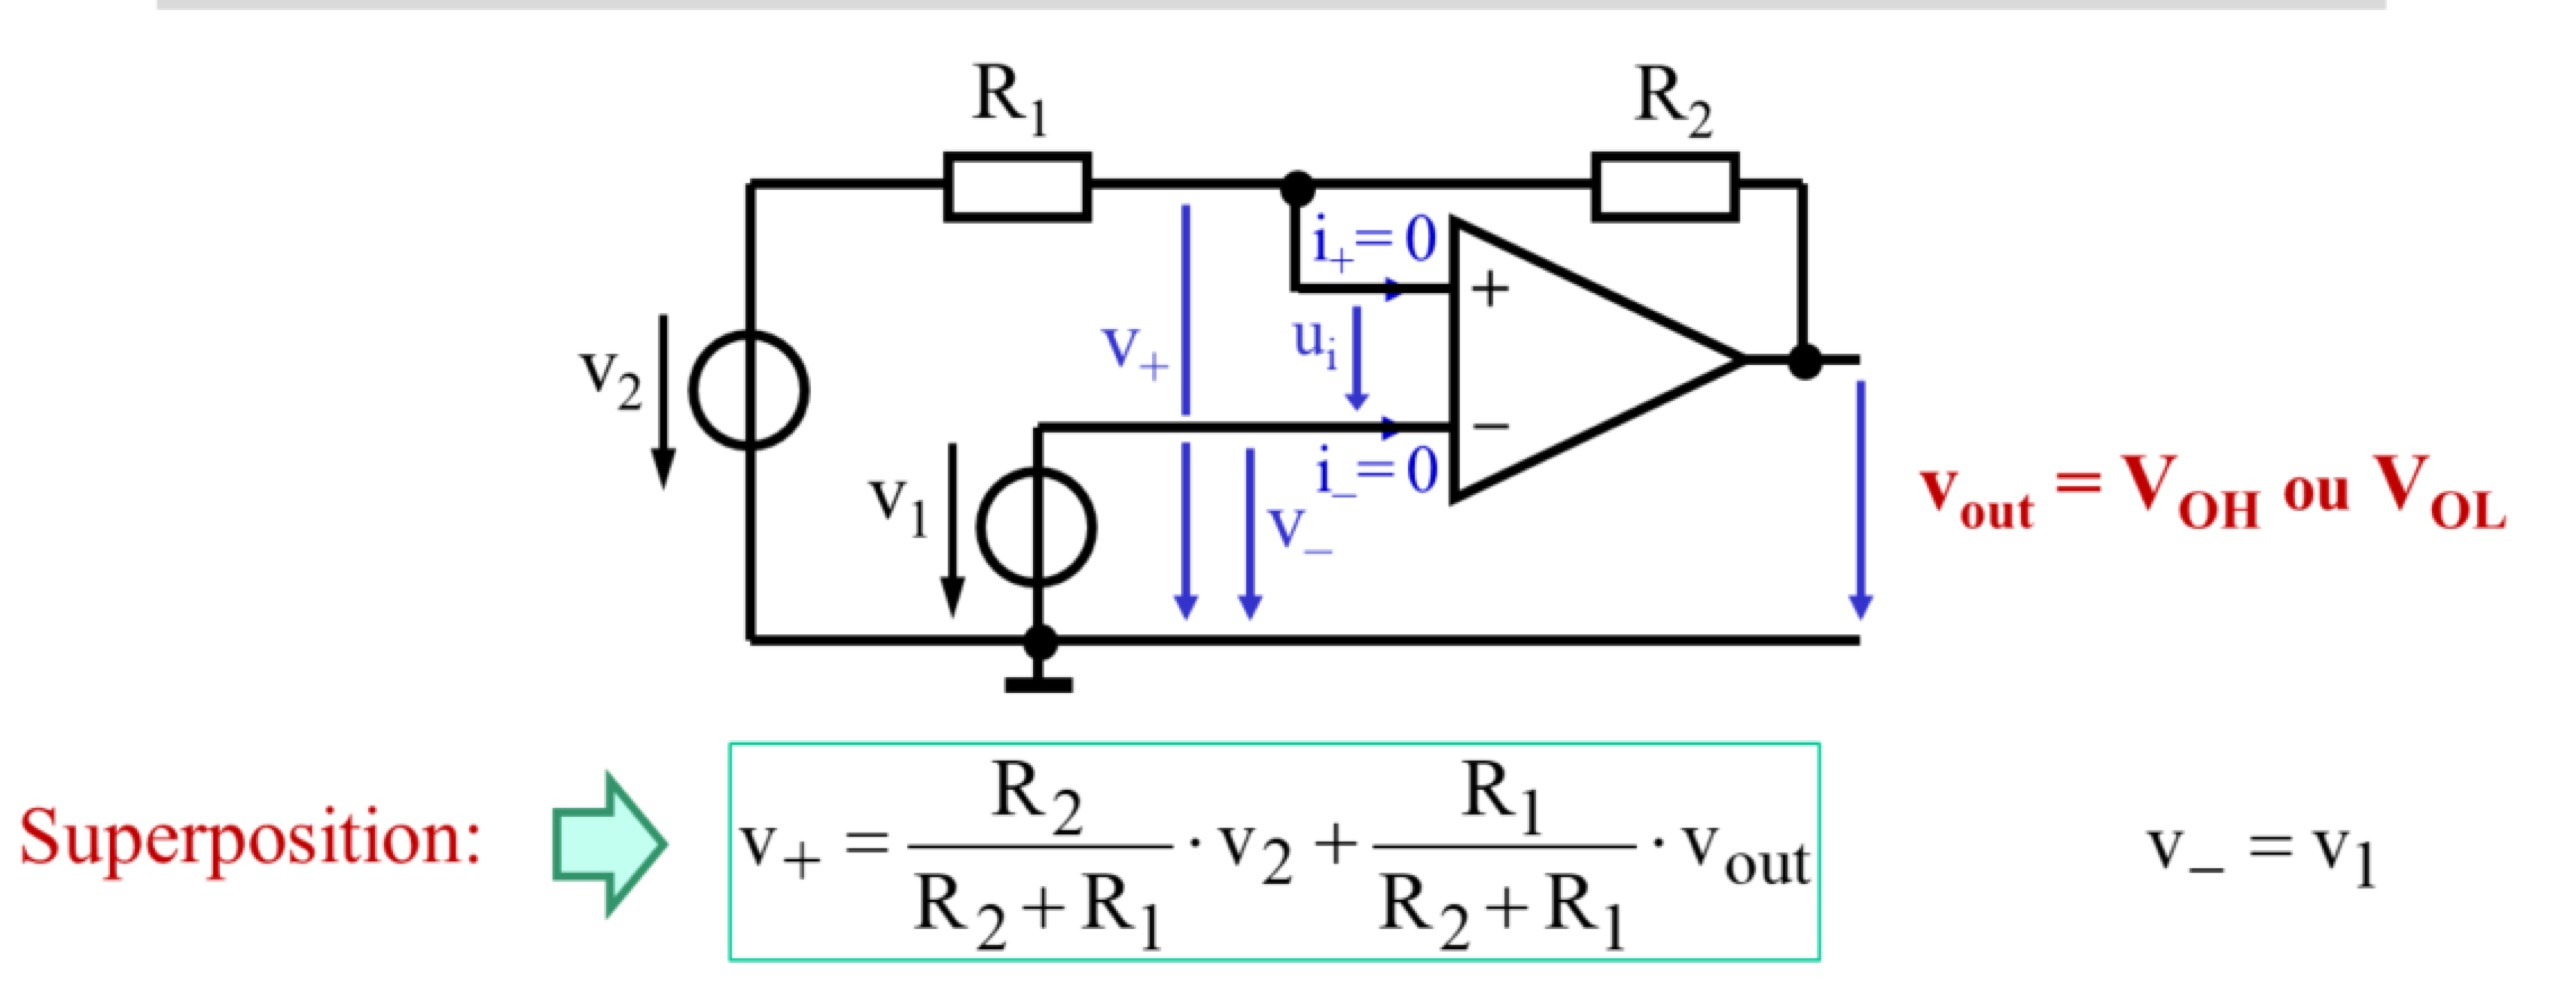
\includegraphics[width=.8\textwidth]{IMAGES/elec/IMG_0148.jpeg}
\end{figure}

\subsubsection{Régime sinus}
Si les sources sont sinusoïdales, on peut alors réécrire les différentes fonctions de transfert avec des impédances : \begin{itemize}
    \item Inverseur : $H(j\omega) = -\frac{Z_2}{Z_1}$\\
    \item Non-inverseur : $H(j\omega) = \frac{Z_2}{Z_1}+1$\\
\end{itemize}

Plusieurs réalisations possibles : \begin{itemize}
    \item Dérivateur (filtre passe-haut) : capacité en série avec la source connectée sur la borne négative de l'AO $H(j\omega) = -j\omega RC$\\
    \item Intégrateur (filtre passe-bas) : capacité dans la branche de réaction négative $H(j\omega) = -\frac{1}{j\omega RC}$\\
\end{itemize}

\warning La tension de sortie ne changera pas si on connecte un autre élément à la suite. 

\subsubsection{Gain Bandwidth}
Un ampli Op a un gain qui diminue au delà d'une fréquence $f_0$\begin{equation}
    \underline{A} = \frac{A_0}{1+j\frac{\omega}{\omega_0}}
\end{equation}

Pour des fréquences $f>f_0$, on a $A\simeq \frac{A_0}{j\frac{\omega}{\omega_0}}$.\\

Alors $\lvert A\rvert f = \lvert A_0 \rvert f_0$ est constant.\\

\textbf{Fréquence de transition} $f_T$ est la fréquence où le gain intrinsèque vaut $\lvert A\rvert =1$ (passe par 0dB dans le Bode plot)\\
\begin{equation}
    f_T=\lvert A_0\rvert f_0 = GBW
\end{equation}

On peut alors redéfinir la fonction de transfert en réaction négative pour ce gain donné. \\
\begin{equation}
    G(j\omega) = \frac{A_0}{1+\beta A_0} \frac{1}{1+ \frac{j\omega}{(1+\beta A_0)\omega_0}}
\end{equation}


Or, $\beta A_0>>1$ alors $H(j\omega) \simeq \frac{1}{\beta} \frac{1}{1+j\frac{f}{f_c}}$ avec $f_c$ la \textbf{fréquence de coupure}. \begin{equation}
    f_c = \beta f_T = \frac{GBW}{G_{non-inv}}
\end{equation}

\subsubsection{Slew rate}
La tension de sortie présente une vitesse de variation $\frac{dv}{dt}$ qui est limitée. \textbf{SR (slew rate)} en $V/\mu s$\\
La pente de $v_{out}$ ne peut pas dépasser le Slew Rate. La déformation provoquée par le Slew Rate est un phénomène non-linéaire qui dépend de l'amplitude du signal de sortie.\\

\subsection{Oscillateurs}
Un générateur de signaux, oscilateur ou bascule astable (sortie binaire) et un circuit qui génère de manière autonome un signal périodique. Pas de signal d'entrée.\\

\subsubsection{Oscillateurs carrés}
Un quadripôle actif avec une sortie binaire et une caractéristique de transfert à hystérèse inverseur, connecté sur lui-même avec un circuit de retard va générer un signal périodique rectangulaire. \\

\begin{itemize}
    \item fréquence : $f = \frac{1}{T} = \frac{1}{T_H+T_L}$\\
    \item rapport cyclique : $d = \frac{T_H}{T}$\\
\end{itemize}

\begin{figure}[hbt!]
    \centering
    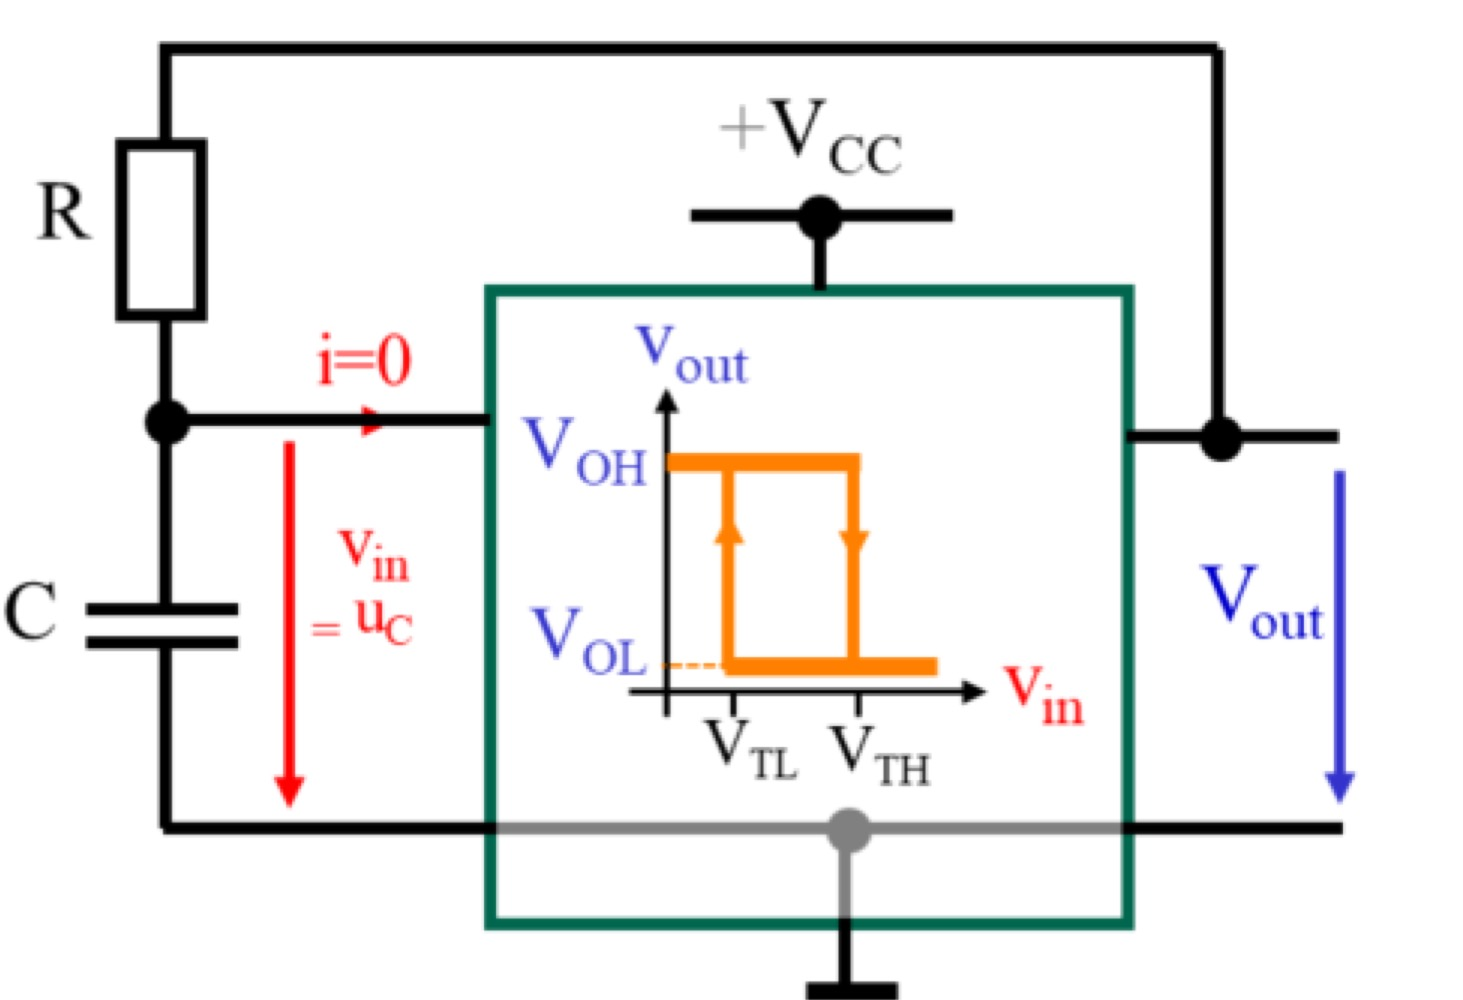
\includegraphics[width=.6\textwidth]{IMAGES/elec/IMG_0149.jpeg}
\end{figure}

On a ici : \begin{equation}
    \begin{gathered}
        T_H = RC\ln(\frac{V_{OH}-V_{TL}}{V_{OH}-V_{TH}})\\
        T_L = RC\ln(\frac{V_{TH}-V_{OL}}{V_{TL}-V_{OL}})\\
    \end{gathered}
\end{equation}

\begin{figure}[hbt!]
    \centering
    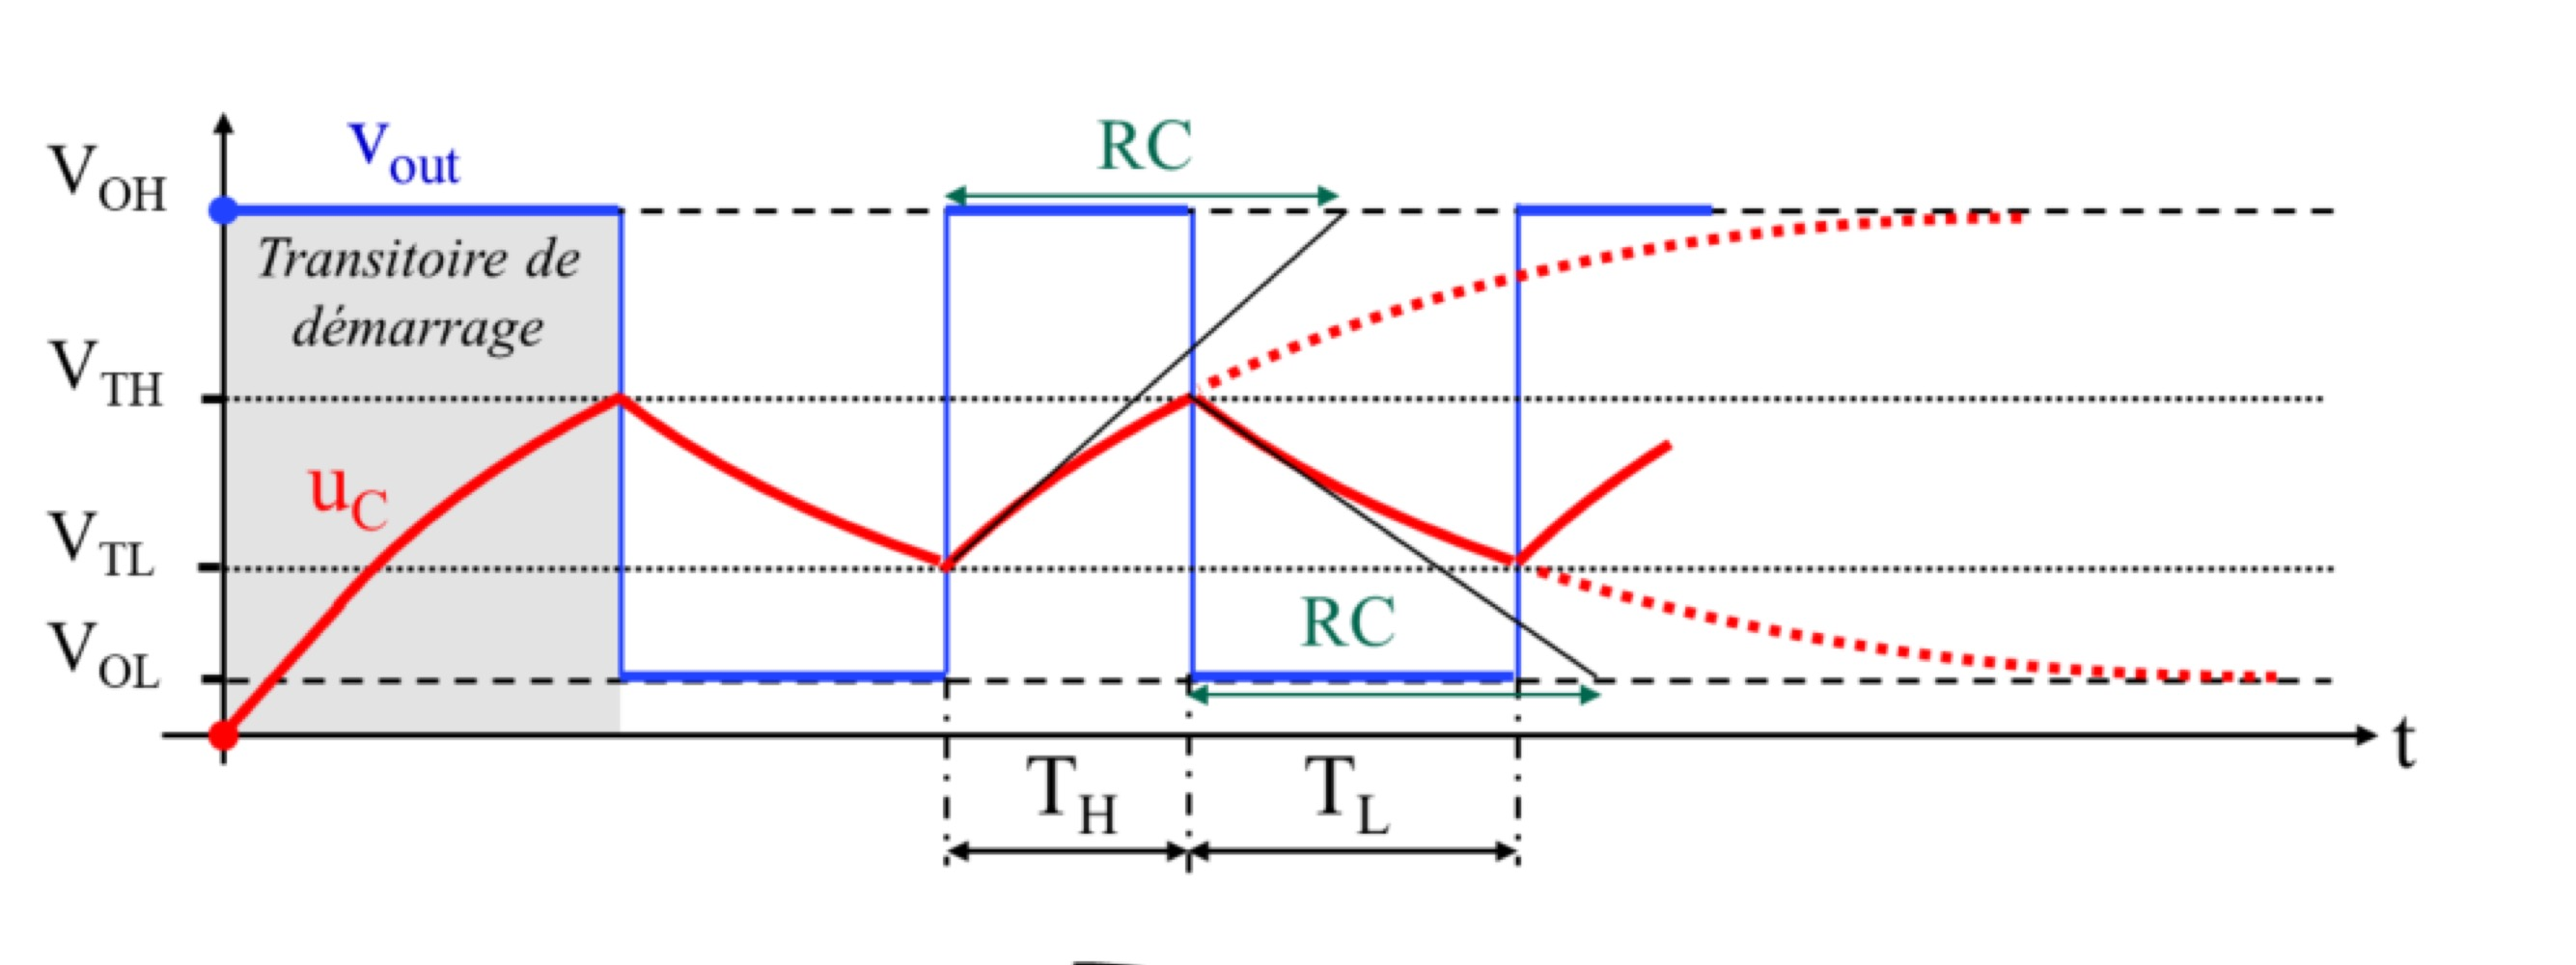
\includegraphics[width=.7\textwidth]{IMAGES/elec/IMG_0150.jpeg}
\end{figure}

On peut également réaliser une bascule astable améliorée où $T_H$ et $T_L$ sont indépendants : \\

\begin{figure}[hbt!]
    \centering
    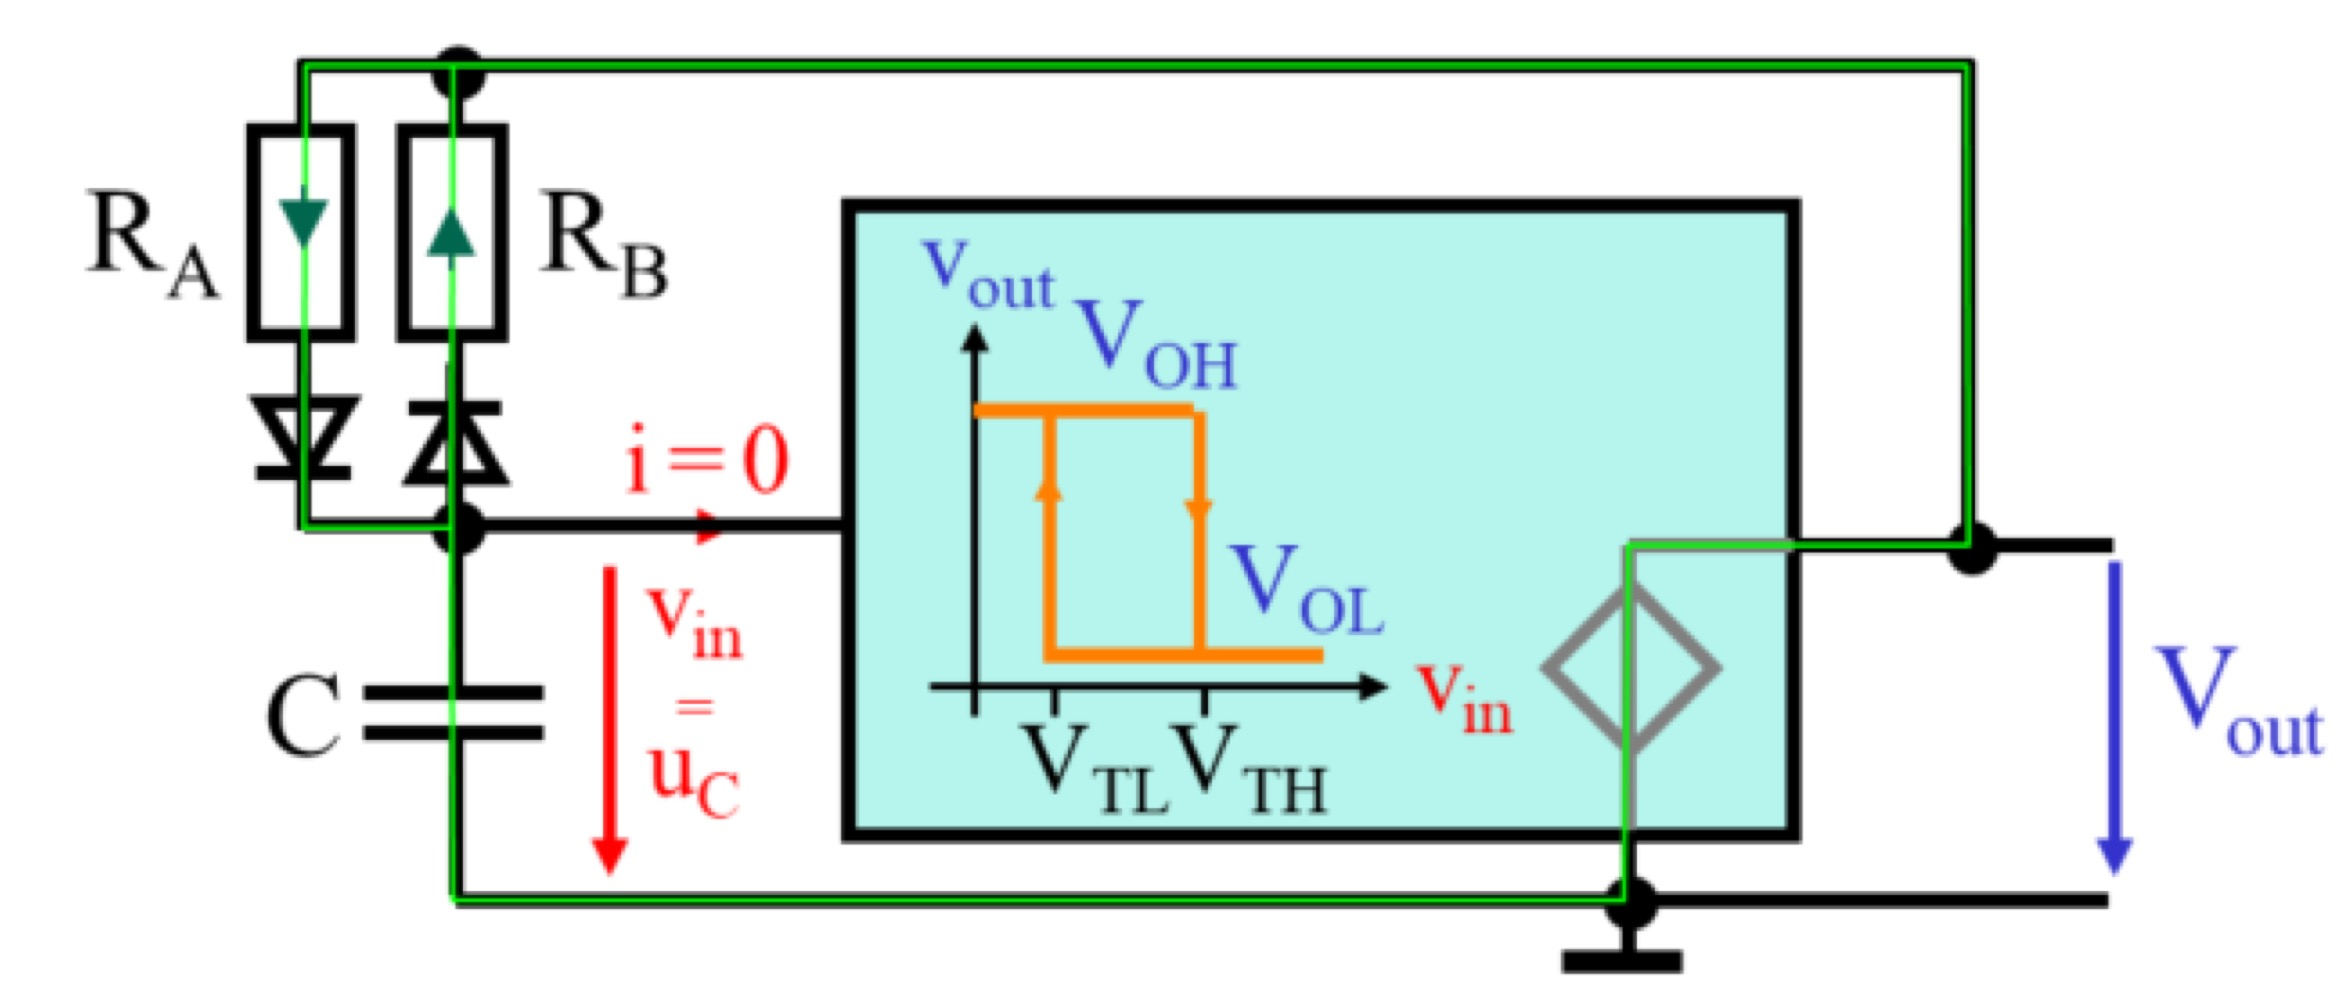
\includegraphics[width=.6\textwidth]{IMAGES/elec/IMG_0151.jpeg}
\end{figure}

Ici : \begin{equation}
    \begin{gathered}
        T_H = R_AC \ln(\frac{V_{OH}-V_{TL}}{V_{OH}-V_{TH}})\\
        T_L = R_BC \ln(\frac{V_{TH}-V_{OL}}{V_{TL}-V_{OL}})\\
    \end{gathered}
\end{equation}

\warning On néglige $U_j$. Si on le prend en compte alors on a $V_{OH} - U_j$ et $V_{OL}+U_j$\\

Avec un ampli op. à alimentation symétrique, on a : \begin{equation}
    \begin{gathered}
        T_H = RC\ln(1+2\frac{R_1}{R_2})\\
        T_L = RC\ln(1+2\frac{R_1}{R_2})\\
        T = 2RC\ln (1+2\frac{R_1}{R_2})\\
    \end{gathered}
\end{equation}
\warning Limité en fréquence par le Slew Rate de l'AO.\\

Si alimentation à seuil unique : $V_{OH} = V_{cc}$ et $V_{OL} = 0$ on a \begin{equation}
    \begin{gathered}
        V_{TH} = (1+\frac{R_1}{R_1+R_2}) \frac{V_{cc}}{2}\\
        V_{TL} = (1-\frac{R_1}{R_1+R_2}) \frac{V_{cc}}{2}\\
        T_H = T_L = RC\ln(1+2\frac{R_1}{R_2})\\
    \end{gathered}
\end{equation}

Générateur de triangles avec 2 AO : \\
On met une alimentation symétrique et deux AO en série : 

\begin{figure}[hbt!]
    \centering
    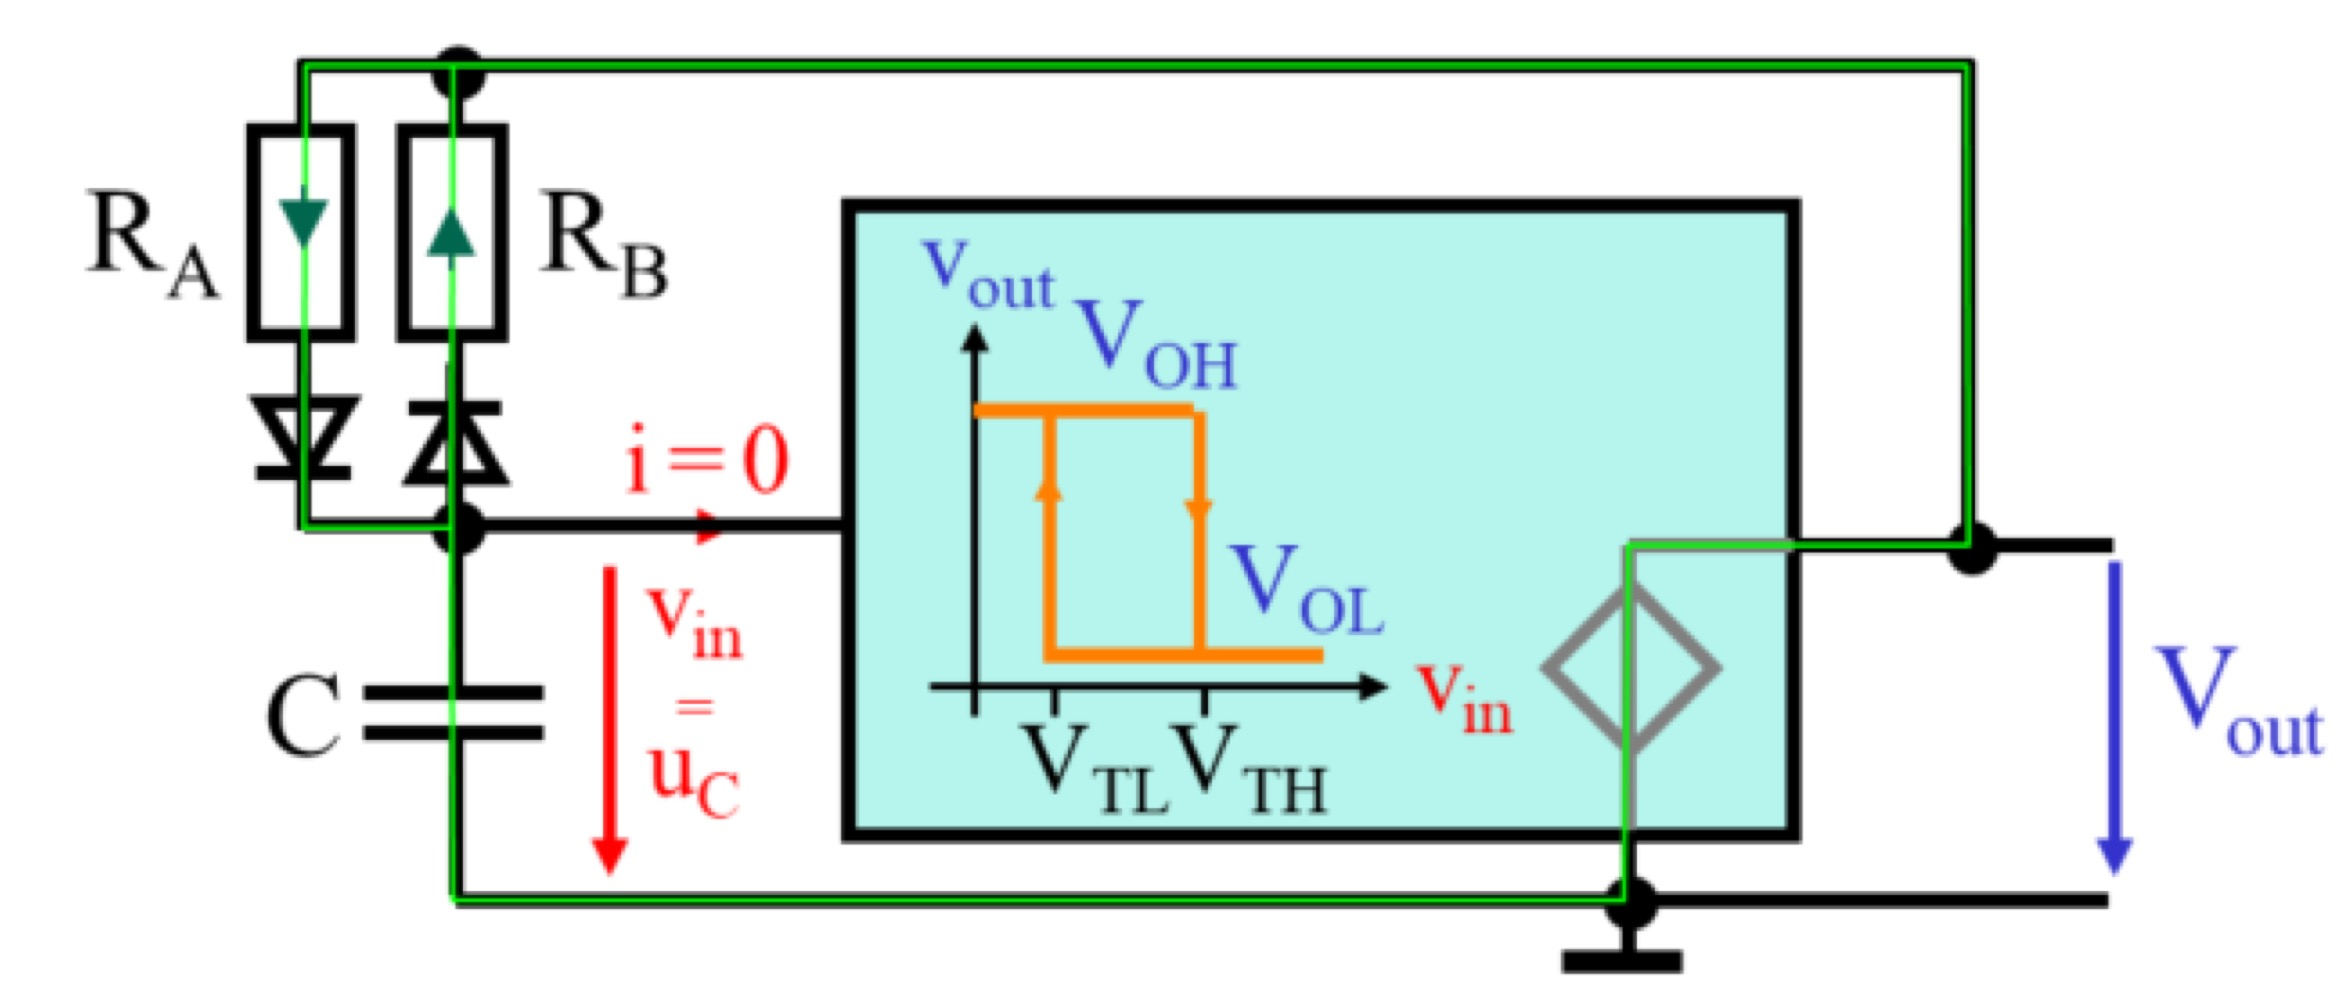
\includegraphics[width=.7\textwidth]{IMAGES/elec/IMG_0151.jpeg}
\end{figure}

On a $T_H = T_L = 2R \frac{R_1}{R_2}$\\

\subsubsection{Oscillateur sinus}
Un quadripôle linéaire avec une fonction de transfert peut générer une oscillation sinusoïdale de pulsation $\omega_{osc}$ et d'amplitude constante lorsque la sortie est rebouclée sur l'entrée.\\

Il existe une pulsation $\omega_{osc} \neq 0$ pour laquelle : \begin{equation}
    \begin{gathered}
        arg H(j\omega_{osc}) = 0\\
        \lvert H(j\omega_{osc})\rvert = 1\\
    \end{gathered}
\end{equation}

Pour que les oscillations démarrent et croissent il faut que $\lvert H(j\omega_{osc})\rvert >1$ lorsque leur amplitude est faible.

\warning $H(j\omega)$, la fonction de transfert du système ouvert.\\

Types : \begin{itemize}
    \item Sinus RC : $f_{osc}$ du Hz au MHz, peu stable, contrôle d'amplitude délicat\\
    \item Sinus LC : $f_{osc}$ du MHz au GHz, stable, contrôle d'amplitude automatique\\
    \item à lignes de transmission : dans les GHz\\
\end{itemize}

On peut également créer un oscillateur sinus grâce à la mise en série de trois AO avec capacité en parallèle avec $R_2$.\\
On a dans ce cas : $\omega_{osc} = \sqrt{3}\frac{1}{CR_2}$ et $R_2=2R_1$\\

\quad \underline{Sinus LC :}\\
L'élément actif se comporte comme une source de courant commandée.\\

\begin{figure}[hbt!]
    \centering
    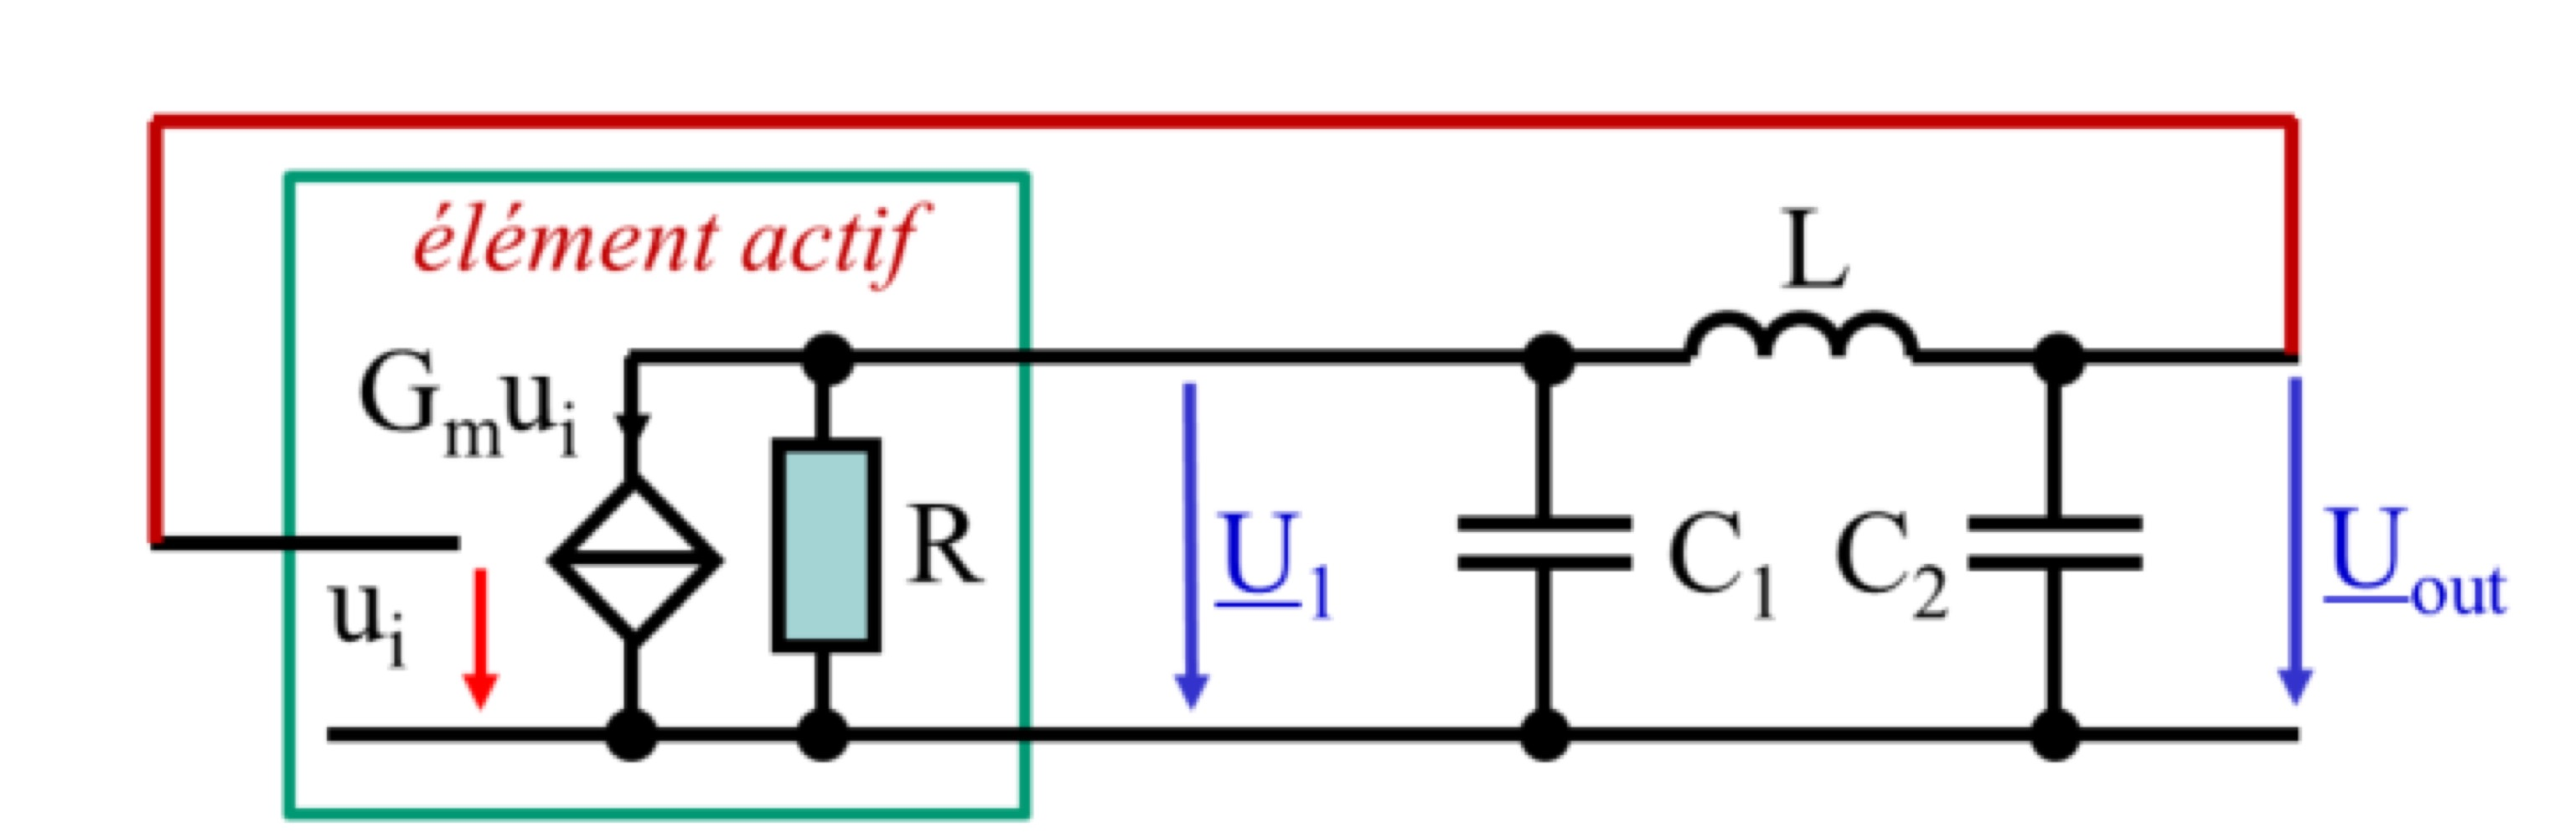
\includegraphics[width=.7\textwidth]{IMAGES/elec/IMG_0153.jpeg}
\end{figure}

Si $G_mR>\frac{C_2}{C_1}$, le circuit va osciller à la fréquence : $f_{osc} = \frac{1}{2\pi \sqrt{L\frac{C_1C_2}{C_1+C_2}}}$\\

$H(j\omega) = -G_m Z_{tot} \frac{Z_{C_2}}{Z_L + Z_{C_2}} = \frac{-G_m R}{1-\omega^2 LC_2 + j\omega R(C_1+C_2 - \omega^2LC_1C_2)}$\\

\quad \underline{Quartz :}\\

On remplace l'inductance par un quartz. On a $f_{osc} = f_Q$.\\

\begin{equation}
    Z_{quartz} = j\frac{-(1-\omega^2LC)}{\omega(C_0+C)(1-\omega^2L\frac{CC_0}{C+C_0})}
\end{equation}

\begin{itemize}
    \item Fréquence où l'impédance s'annule : $\omega_s = \frac{1}{\sqrt{L_mC_m}}$\\
    \item Fréquence où l'impédance devient infinie : $\omega_p = \frac{1}{\sqrt{L_m \frac{C_mC_0}{C_m+C_0}}}$\\
\end{itemize}

\subsection{Circuits numériques logique}
\subsubsection{Traitements numériques des signaux}

\begin{itemize}
    \item Monde analogique : grandeurs à variation continue. Un continuum de valeurs possibles \\
    \item Monde numérique : grandeurs à valeurs discrètes. Un nombre fini de valeurs possibles\\
\end{itemize}

\begin{itemize}
    \item Avantages : \begin{itemize}
        \item Insensibilité au bruit\\
        \item Précision\\
        \item Souplesse\\
    \end{itemize}
    \item Inconvénients : \begin{itemize}
        \item Conversion A/N et N/A\\
        \item Complexité\\
        \item Temps de traitement\\
    \end{itemize}
\end{itemize}

Cependant, ces inconvénients sont minimisés par l'augmentation des performances des circuits intégrés.\\

\subsubsection{Algèbre de Boole}

Soit un chiffre en bit : $a_i = [1,0]$\\
La représentation d'un nombre en base 2 : $a_{n-1} a_{n-2}\dots a_0$\\
Soit la valeur d'un chiffre binaire : \begin{equation}
    A = \sum_{i=0}^{n-1} a_i 2^i
\end{equation}

Avec : \begin{itemize}
    \item MSB : most significant bit, le bit de poids le plus fort ($2^{n-1}$)\\
    \item LSB : least significant bit, le bit de poids le plus faible ($2^0$)\\
\end{itemize}

Une variable binaire ne peut avoir que deux valeurs appelées États : \begin{itemize}
    \item Valeur logique : 1, équivalent électrique 5Volts-High, équivalent électrique : close\\
    \item 0, 0Volts-Low, open\\
\end{itemize}

\quad \underline{Opérateurs logiques binaires fondamentaux :}\\

\begin{figure}[hbt!]
    \centering
    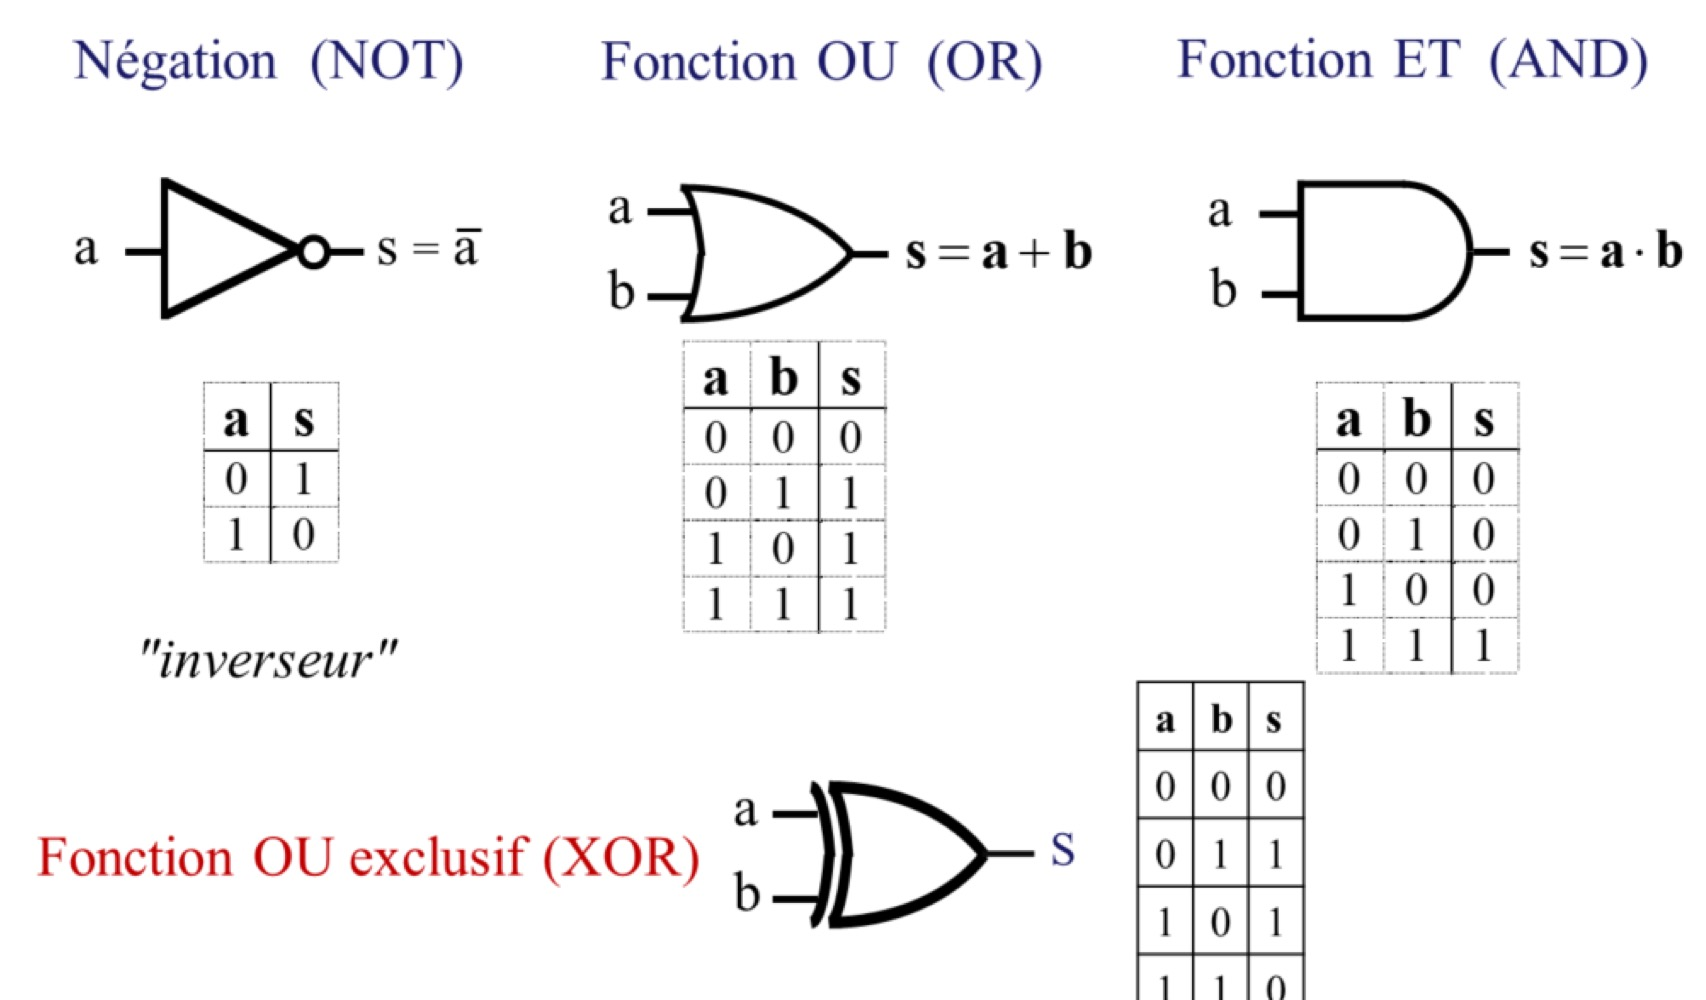
\includegraphics[width=.7\textwidth]{IMAGES/elec/IMG_0155.jpeg}
\end{figure}

\begin{itemize}
    \item Commutativité : $ab = ba$, $a+b = b+a$\\
    \item Distributivité : $a(b+c) = (ab)+(ac)$, $a+(bc) = (a+b)(a+c)$\\
    \item Associativité : $a(bc) = (ab)c = abc$, $a+(b+c) = a+b+c$\\
    \item Consensus : $(ac)+ (b\overline{c}) + (ab) = (ac) + (b \overline{c})$, $(a+c) (b+\overline{c}) (a+b) = (a+c) (b +\overline{c})$, $a+(ab) = a$, $a+(\overline{a}b) = a+b$\\
    \item Loi De Morgan : $\overline{ab} = \overline{a}+ \overline{b}$\\
\end{itemize}

Il existe aussi les portes NOR et NAND qui combinent les portes not et and avec des not en sortie.\\
\warning La porte logique XOR a pour fonction : $s = (a\overline{b})+(b\overline{a})$\\

Le temps de réaction d'un opérateur logique est modélisé par un élément de retard à la sortie de l'opérateur idéal. Il introduit \textbf{un temps de propagation $t_p$ entre un changement d'état de sa sortie vis-à-vis de son entrée.} Un intervalle de temps inférieur à $t_p$ n'aura aucun effet sur la sortie.\\


\subsubsection{Logique combinatoire}
A chacune des $2^n$ combinaisons des entrées $x_i$ correspond une valeur de sortie. \\
Toute fonction combinatoire peut être décomposé en une somme de produits des entrées ou de leurs inverses.\\

\subsubsection{Élément de mémoire et bascule}

\begin{figure}[hbt!]
    \centering
    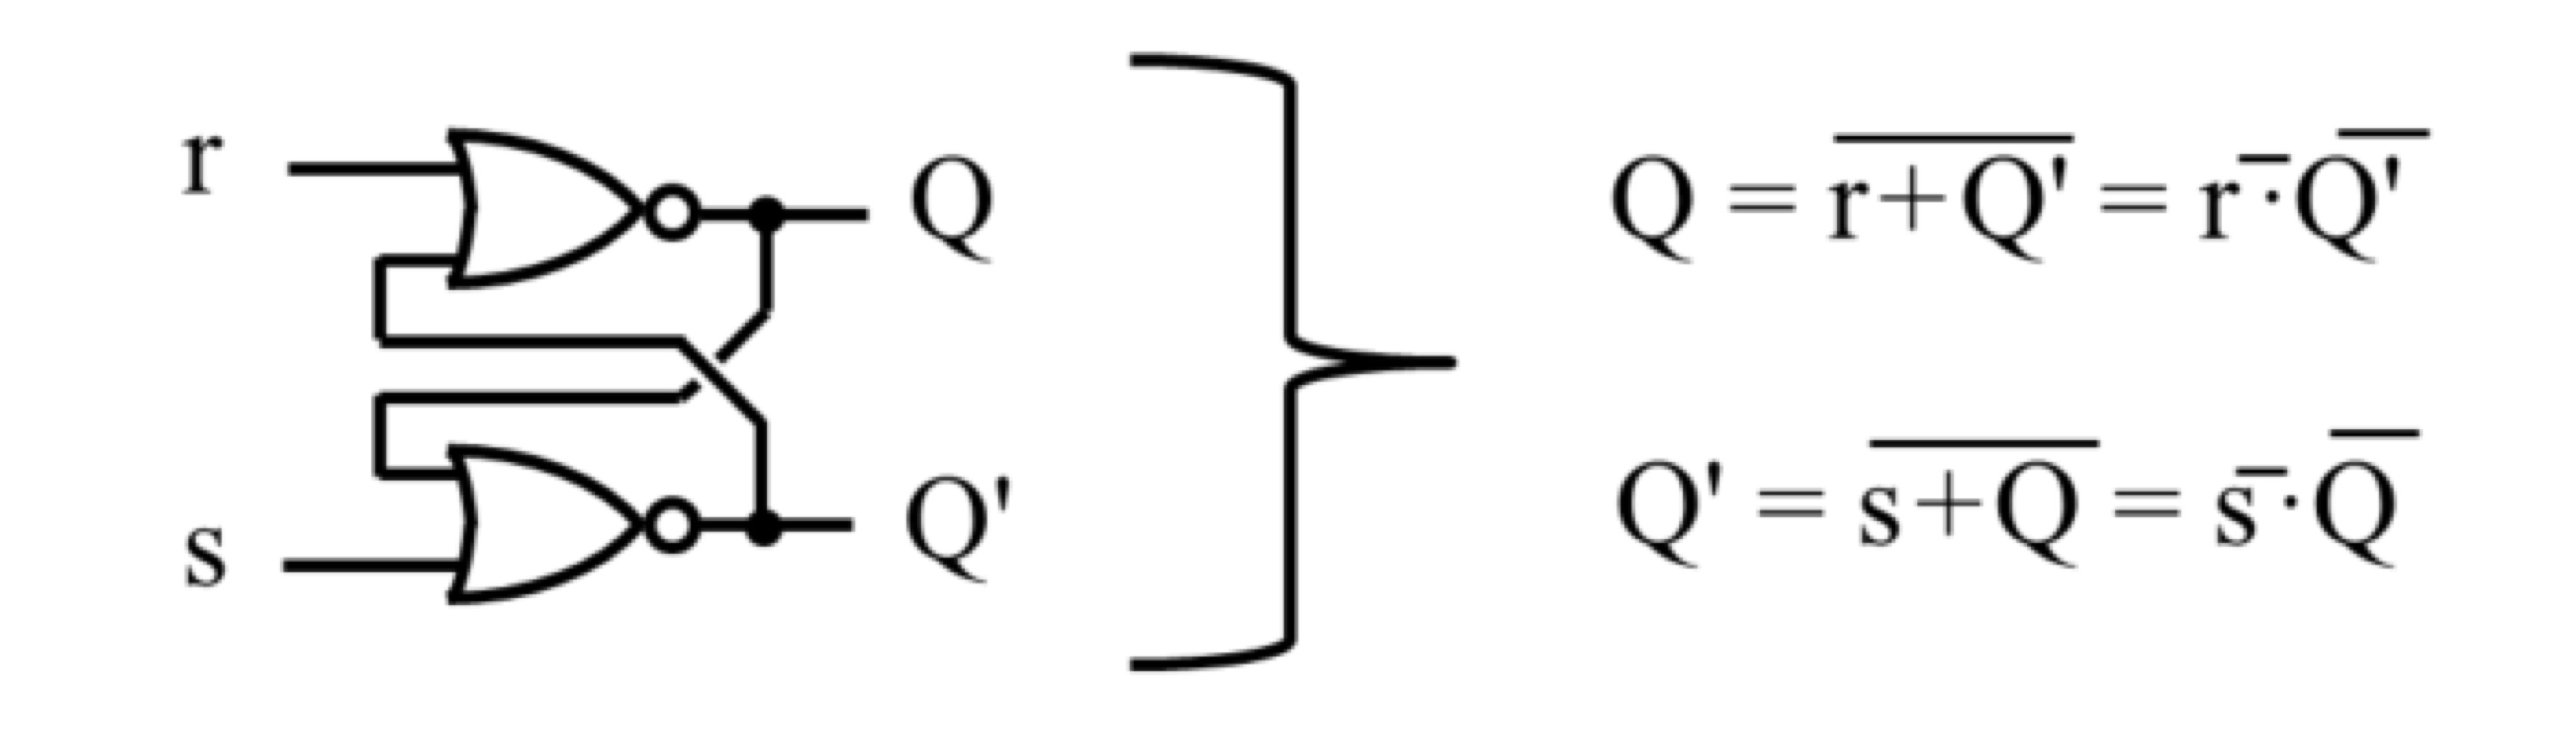
\includegraphics[width=.6\textwidth]{IMAGES/elec/IMG_0156.jpeg}
\end{figure}

\begin{table}[hbt!]
    \centering
    \begin{tabular}{c|c|c}
       s=0 et r=1  & Q=0 et $Q'=\overline{Q} =1$ & Q est mis à 0, reset \\ \hline
        s=1 et r=0 & $Q'=0$ et $Q = \overline{Q'}=1$ & Q est mis à 1, set\\ \hline
        s=0 et r=0 & $Q'= \overline{Q}$ et $Q = \overline{Q'}=Q$ & état stable\\
    \end{tabular}
\end{table}

Cela garde donc en mémoire même s'il n'est pas alimenté.\\

\quad \underline{D-type Edge Triggered Flip Flop Bascule D :}\\

Au front montant du signal d'horloge CK, l'état de l'entrée D est envoyé sur la sortie Q. Cette sortie garde sa valeur jusqu'au prochain front montant de CK, même si l'entrée D change entre temps.\\

\begin{figure}[hbt!]
    \centering
    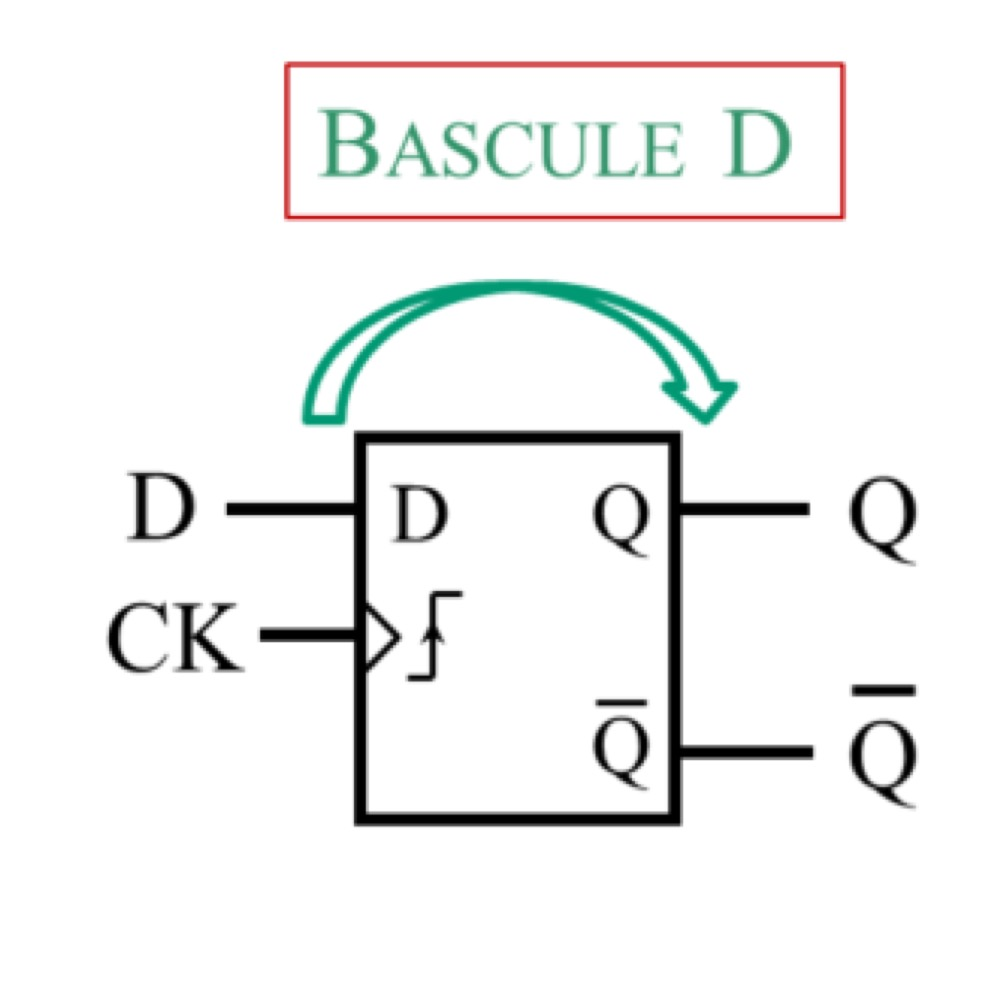
\includegraphics[width=.6\textwidth]{IMAGES/elec/IMG_0157.jpeg}
\end{figure}

Ainsi, lors du front montant de CK, on a $Q^+ = D$.\\

\subsubsection{Systèmes logiques séquentiels synchrones}
On combine une logique combinatoire avec des bascule D toute régit selon la même horloge CK. \\
Juste après le front montant du signal d'horloge CK, chaque bascule prendre un nouvel état $Q_i^+ = D_i$ qui est une fonction combinatoire des états présents de toutes les bascules $Q_0$ à $Q_n$ et de toutes les entrées $X_0$ à $X_m$ à l'instant du front d'horloge.\\


\subsubsection{Systèmes logiques séquentiels asynchrones}
Cette fois-ci, les bascule D n'ont pas la même horloge CK.\\
Chaque bascule peut avoir son propre signal d'horloge, ou elle peut être forcée à 1(set) ou 0(reset) à tout instant autre qu'au front de son horloge. \\

\quad \underline{Comparatif synchrones vs asynchrones :}\\

\begin{itemize}
    \item Synchrones : \begin{itemize}
        \item temps de propagation du front d'horloge identique : synchronisation des entrées\\
        \item optimum pour la rapidité\\
        \item système combinatoire complexe\\
    \end{itemize}
    \item Asynchrones : \begin{itemize}
        \item temps de propagation variable d'une entrée\\
        \item risques d'états transitoires parasites\\
        \item diminue la complexité du système combinatoire associé\\
    \end{itemize}
\end{itemize}

\subsubsection{Sortie 3 états}
Un système combinatoire peut avoir une autre entrée E dite d'activation. Elle permet de commander l'interrupteur qui lie le système logique à la sortie.\\

On a alors la sortie du système logique $s^*$ et la sortie du système global : $s = s^* [0,1]$.\\
$s$ est la sortie à trois états.\\

\subsection{Conversions AN NA}
\subsubsection{Convertisseur N/A}
Soit une entrée numérique $N_{in}$. On quantifies les échantillons, on lisse le résultat et on a la sortie analogique $U_{out}$.\\

\quad \underline{Uni-polaire à n bits :}\\
Un convertisseur NA transforme un nombre $N_{in}$ codé sur n bits en base 2 en une grandeur analogique : \begin{equation}
    U_{out} = \frac{U_{ref}}{2^n}N_{in} = \frac{U_{ref}}{2^n} (b_{n-1}2^{n-1} + \dots + b_0 2^0)
\end{equation}
La tension de référence $U_{ref}$ est un paramètre externe appliqué au convertisseur.\\

\quad \underline{Bi-polaire :}\\
On peut représenter des tensions négatives également. Pour ce on définie des nombres binaires décalées de $2^{n-1}$ : \begin{equation}
    \begin{gathered}
        U_{out} = -U_{ref} + \frac{U_{ref}}{2^{n-1}}(b_{n-1} 2^{n-1} + \dots + b_02^0)\\
        N'_{in} = N_{in} - 2^{n-1}\\
        U_{out} = \frac{U_{ref}}{2^{n-1}}N'_{in}\\
    \end{gathered}
\end{equation}

\warning Cela emmène moins de résolution.\\

\subsubsection{Convertisseur A/N}
Soit une entrée analogique $U_{in}$. On échantillonne le signal et on obtient une sortie numérique $N_{out}$.\\

\quad \underline{Uni polaire :}\\
Ce convertisseur transforme une grandeur analogique en un nombre codé en binaire sur n bits suivant : \begin{equation}
    N_{out} = b_{n-1}2^{n-1} + \dots + b_02^0 = \text{Round}_{base2} (2^n \frac{U_{in}}{U{out}})
\end{equation}
$b_i =$ 0 ou 1\\
\warning $U_{ref}$ est fonction de $U_{in,max}$.\\

\quad \underline{Bi-polaire :}\\
Si la grandeur analogique d'entrée du convertisseur est positive ou négative, la sortie sera :\begin{equation}
    \begin{gathered}
        N_{out} = \text{Round}_{base2} ( 2^n \frac{U_{in}+U_{ref}}{2U_{ref}}) = b_{n-1}2^{n-1} + \dots + b_02^0\\
        N'_{out} = N_{out}-2^{n-1} = \text{Round}_{base2} (2^n \frac{U_{in}}{2U_{ref}})\\
    \end{gathered}
\end{equation}
\warning Le pas de quantification est double.\\

\subsubsection{Caractéristiques statiques}

\quad \underline{Dynamique :} \\
Il s'agit de la \textbf{plage utile de la grandeur analogique}. En général : \begin{itemize}
    \item cas uni-polaire : $0\leq U_{out} \leq U_{ref}$\\
    \item cas bi-polaire : $-U_{ref} \leq U_{out} \leq U_{ref}$\\
\end{itemize}

La valeur maximale de sortie d'un CNA uni-polaire est appelée "Full scale"\\

\quad \underline{Nombre de bits et résolution (pas de quantification) :}\\
La résolution dépend du nombre de bits n utilisés pour coder en binaire la grandeur numérique.\\
Il s'agit du plus petit écart de la valeur analogique que peut générer un CNA/détecter un CAN\\

\begin{itemize}
    \item uni-polaire : $\Delta U_q = \frac{U_{ref}}{2^n}$\\
    \item bi-polaire : $\Delta U_q = \frac{U_{ref}}{2^{n-1}}$\\
\end{itemize}

\subsubsection{Caractéristiques temporelles}

\quad \underline{Temps d'établissement :}\\
Le "settling time" est le temps que met le CNA pour atteindre sa valeur maximale.\\

\quad \underline{Fréquence de conversion NA :}\\
Nombre maximal de conversions que le CNA peut effectuer par seconde/nombre maximal de valeurs d'entrée par seconde.\\

\quad \underline{Temps de conversion :}\\
Temps nécessaire pour obtenir une valeur numérique avec un CAN.\\

\quad \underline{Fréquence de conversion AN :}\\
Fréquence d'échantillonnage; nombre maximal de conversions que le CAN peut effectuer par seconde.\\
En général : $f_{conv} \leq \frac{1}{t_{conv}}$\\

\subsubsection{Interface numérique}
Il existe deux types différents.\\


\quad \underline{Interface parallèle :}\\
Chaque bit a une connexion dédiée. Ils sont tous lus/écrits au même instant.\\


\begin{figure}[hbt!]
    \centering
    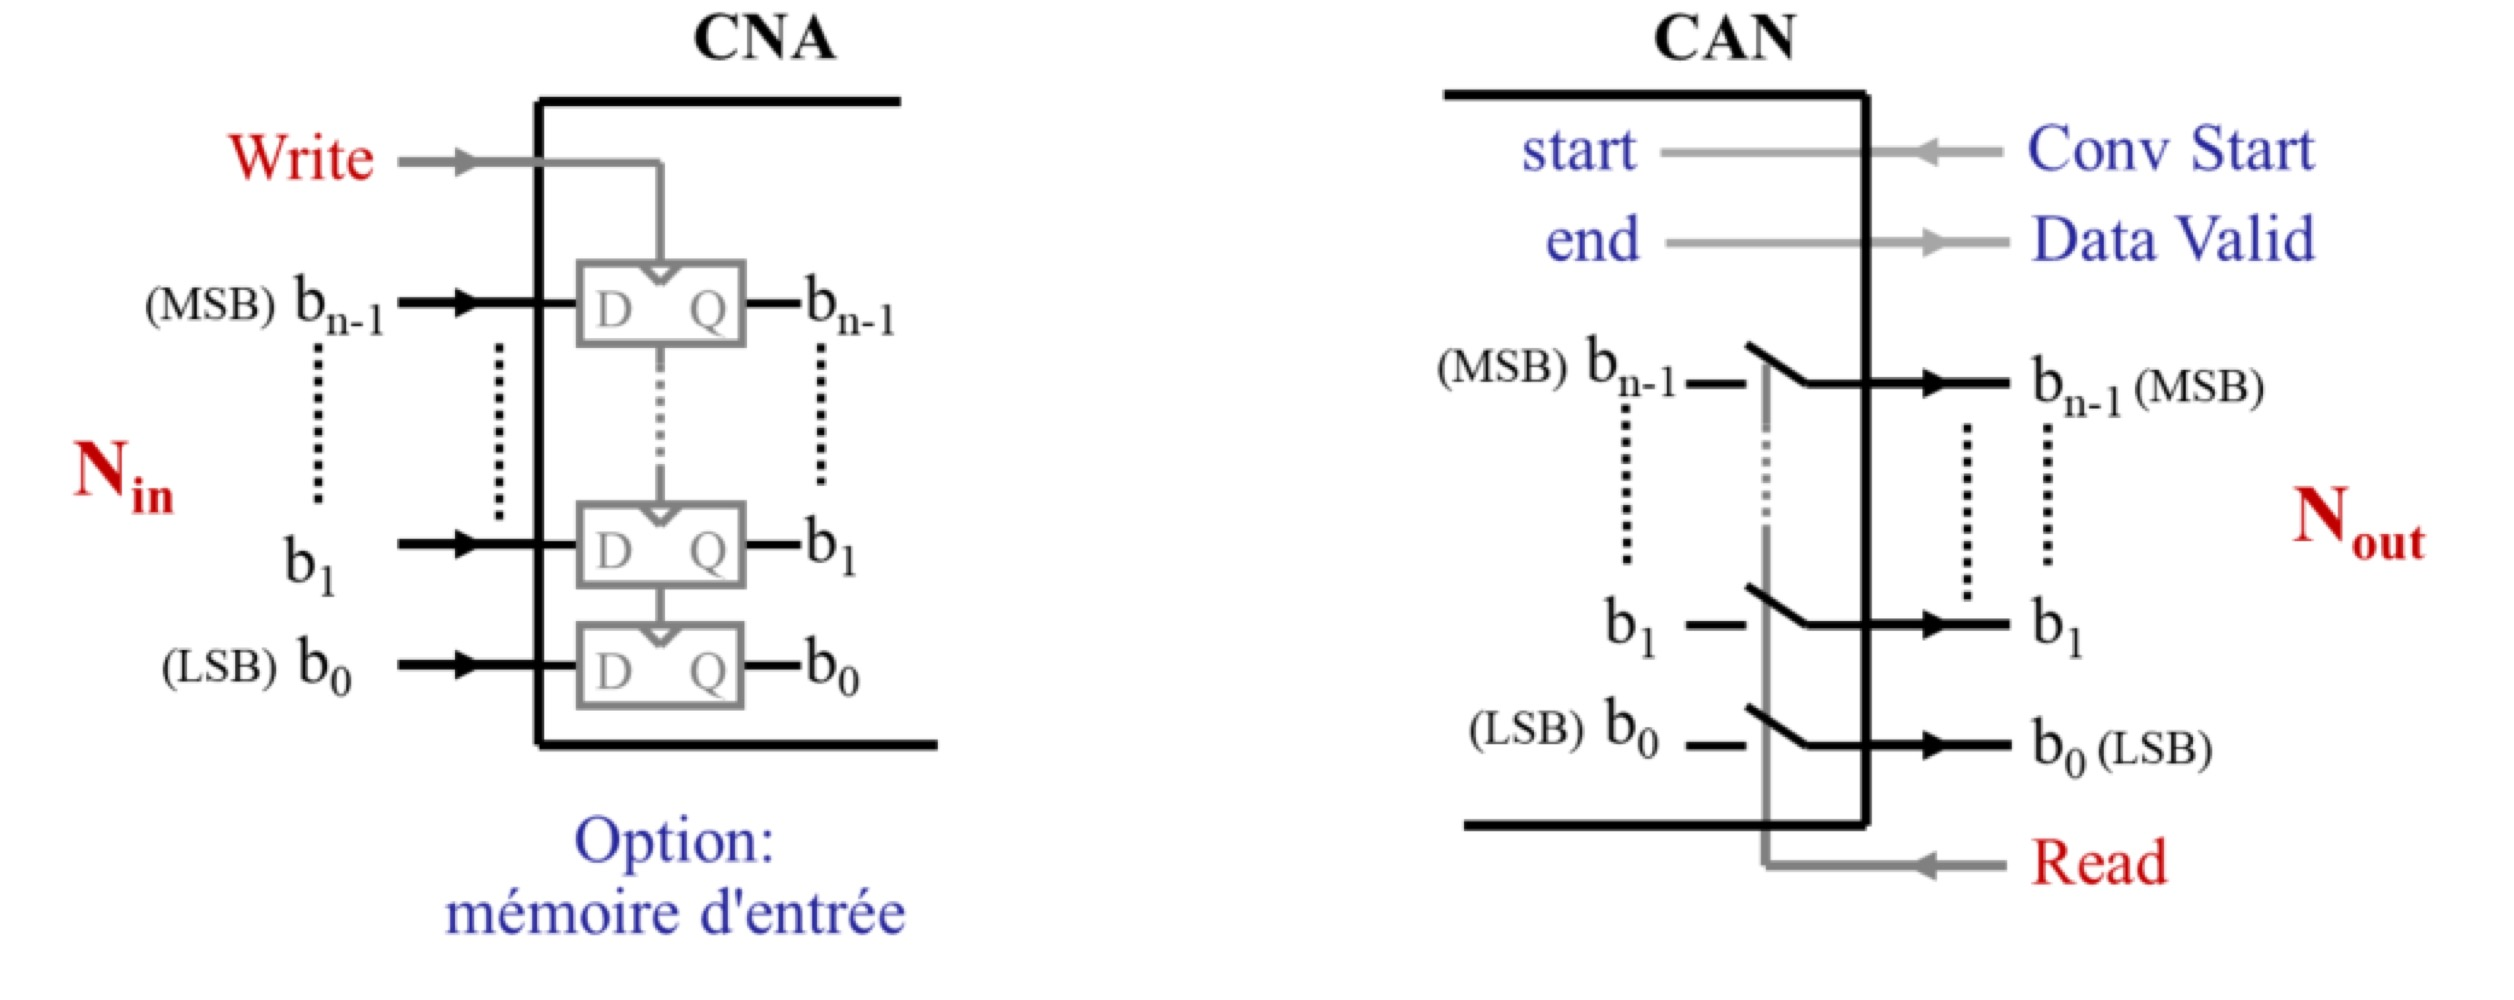
\includegraphics[width=.6\textwidth]{IMAGES/elec/IMG_0162.jpeg}
\end{figure}

\quad \underline{Interface série :}\\
Les bits sont transmis l'un après l'autre sur une connexion unique. On utilise des bascules.\\

\begin{figure}[hbt!]
    \centering
    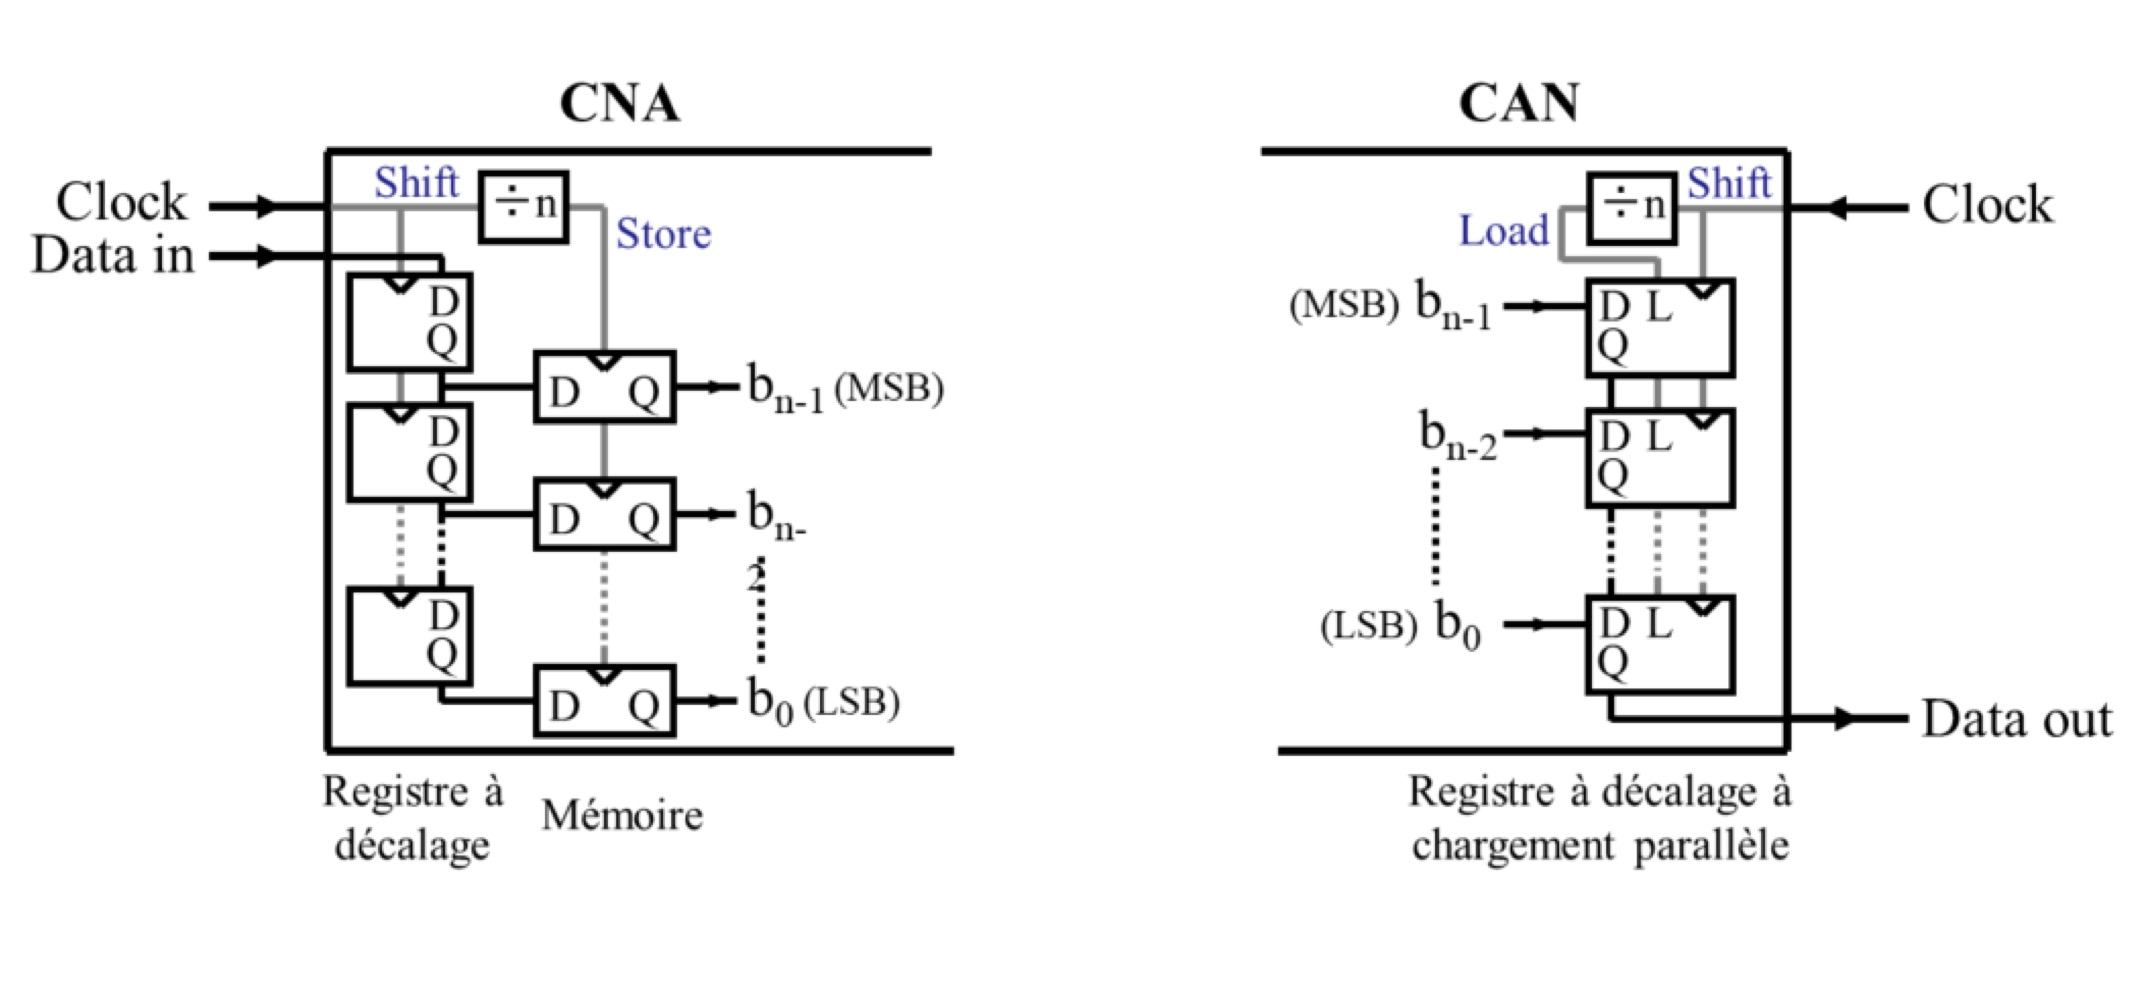
\includegraphics[width=.6\textwidth]{IMAGES/elec/IMG_0163.jpeg}
\end{figure}
Les bits sont successivement transmis à la bascule suivante jusqu'à ce que toutes soient remplis.\\

\subsubsection{Échantillonnage et maintien}
Un échantillonneur à maintien est un circuit qui prend un échantillon de $U_{in}$ à un instant précis et conserve cette valeur durant la durée de la conversion.\\




\underline{Théorème d'échantillonnage :}\\
\begin{theorem}
    Pour qu'un signal puisse être reconstruit, il faut que la fréquence d'échantillonnage soit supérieur au double de la fréquence la plus élevée du signal.\begin{equation}
        f_{ech} \geq 2f_{signal}
    \end{equation}
\end{theorem}
\begin{figure}[hbt!]
    \centering
    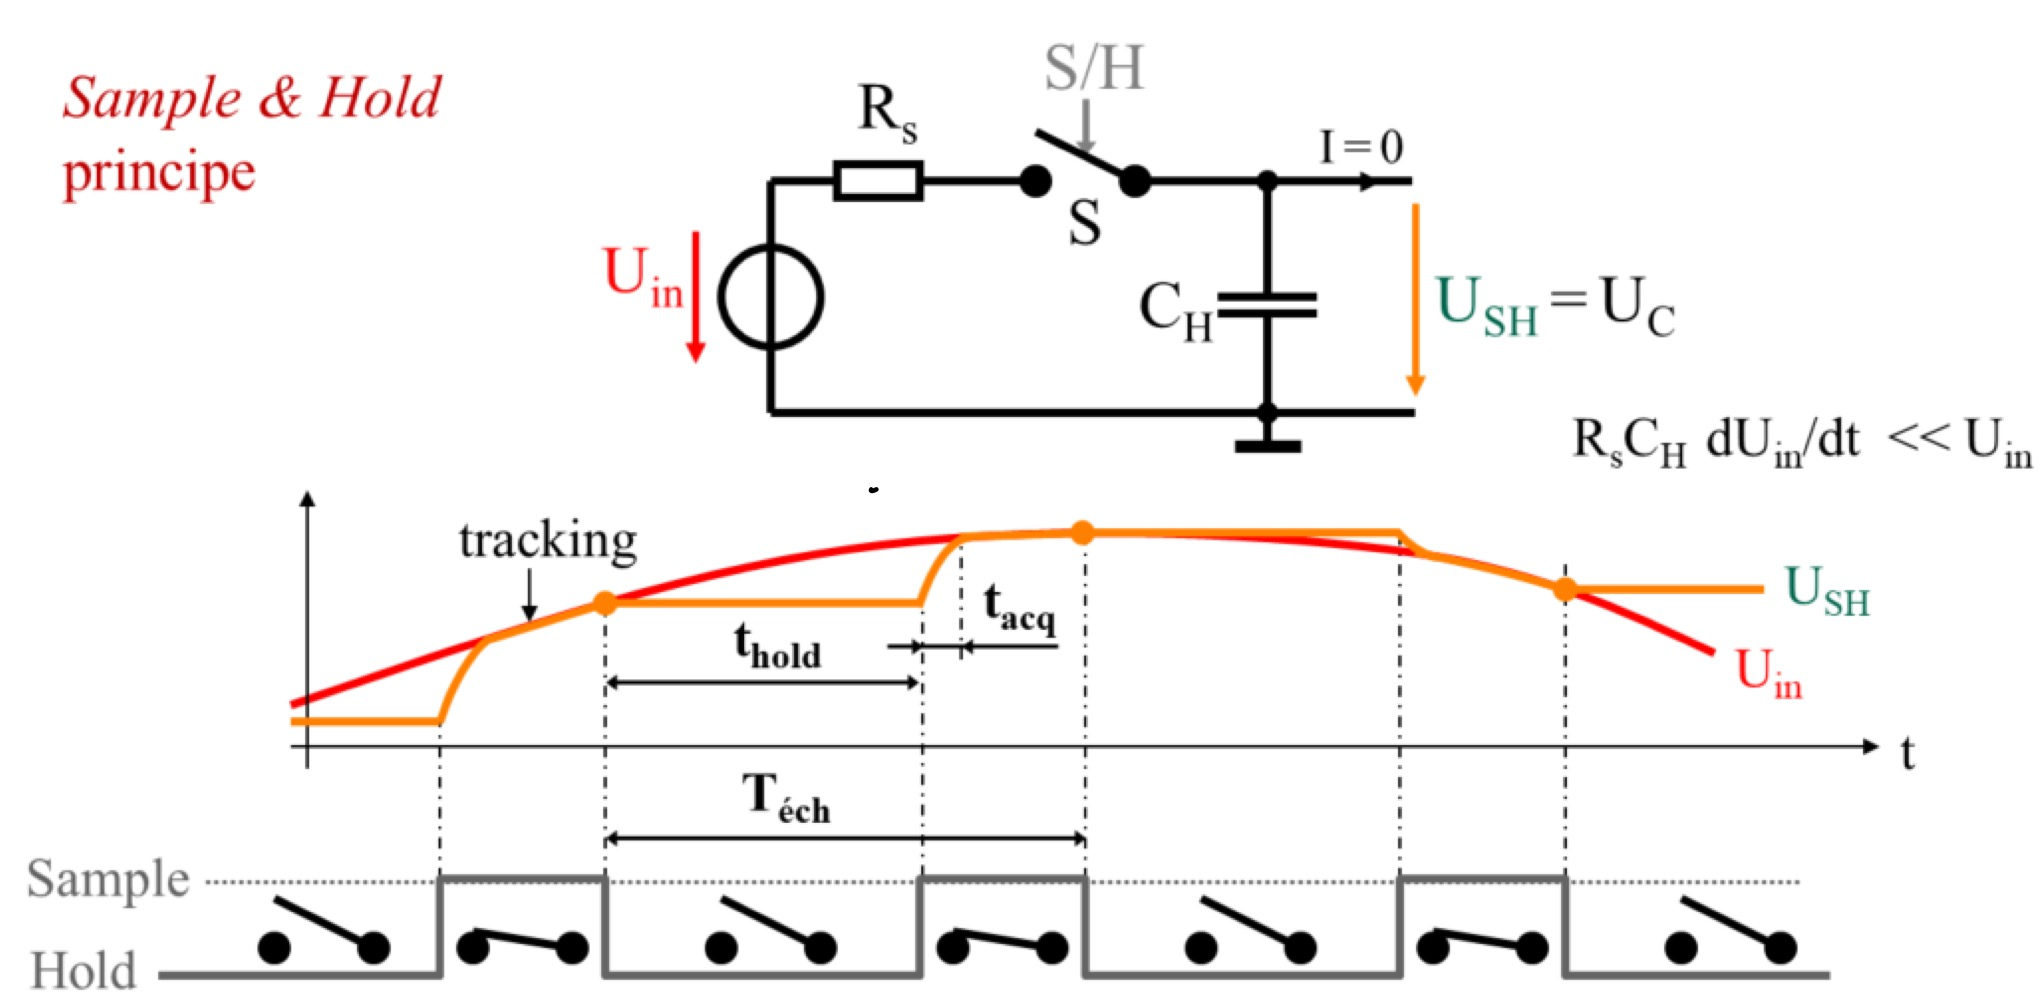
\includegraphics[width=.5\textwidth]{IMAGES/elec/IMG_0164.jpeg}
\end{figure}

\subsection{Transistors MOSFETs}
Metal Oxyde Semi-conducteur Field Effect Transistor\\

Il existe deux types : \begin{itemize}
    \item type N : drain et source de type N et semi-conducteur de type P\\
    \item type P : drain et source de type P et semi-conducteur de type N\\
\end{itemize}
On peut modifier deux facteurs géométriques : W et L\\

\begin{figure}[hbt!]
    \centering
    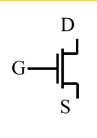
\includegraphics[width=.4\textwidth]{IMAGES/elec/Screenshot from 2023-12-11 13-35-03.png}
\end{figure}

\subsubsection{N-MOSFET}



Si $V_{GS} = 0$ pas de courant entre drain et source, circuit ouvert\\

Lorsque $V_{GS}$ dépasse une tension de seuil $V_T$, il y a création d'un canal de conduction entre le drain et la source.\\

Il y a trois modes de fonctionnement : \begin{itemize}
    \item weak inversion : $V_{GS} < V_T$\\
    \item moderate inversion : $V_{GS} \simeq V_T$\\
    \item strong inversion : $V_{GS}>V_T$\\
\end{itemize}

\begin{figure}[hbt!]
    \centering
    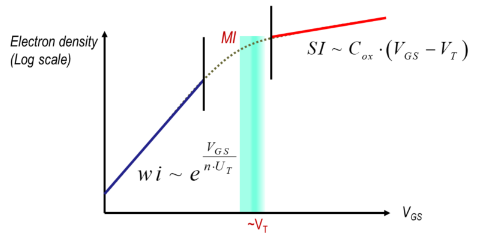
\includegraphics[width=.4\textwidth]{IMAGES/elec/Screenshot from 2023-12-11 13-40-11.png}
\end{figure}

\quad \underline{Forte inversion :}\\

Deux régimes possible : \begin{itemize}
    \item \textbf{Régime saturation :} \begin{equation}
        \begin{gathered}
            V_{GS} >V_T \text{ et } V_{DS} > V_{GS}-V_T\\
            I_{Dsat} = \frac{\beta}{2}(V_{GS}-V_T)^2\\
        \end{gathered}
    \end{equation}
    \item \textbf{Régime linéaire :}\begin{equation}
        \begin{gathered}
            V_{GS} > V_T \text{ et } V_{DS} < V_{GS}-V_T\\
            I_{Dlin} = \beta V_{DS} (V_{GS}-V_T-\frac{V_{DS}}{2})\\
        \end{gathered}
    \end{equation}
\end{itemize}

\begin{figure}
    \centering
    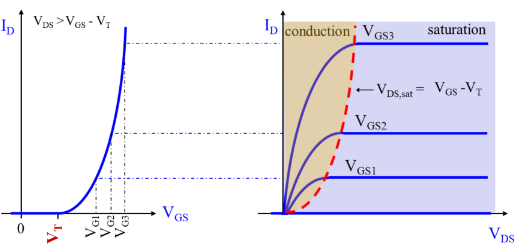
\includegraphics[width=.5\textwidth]{IMAGES/elec/Screenshot from 2023-12-11 13-48-17.png}
\end{figure}

\quad \underline{Paramètre technologique $\beta$ :}\\
\begin{equation}
    \beta = \mu C_{ox} \frac{W}{L}
\end{equation}
En général : \begin{itemize}
    \item mobilité $\mu = 0.1 m^2V^{-1}s^{-1}$\\
    \item capacité de l'oxyde : $C_{ox} = 0.017 F/m^2$\\
    \item $\beta = 0.0017 \frac{W}{L}$\\
\end{itemize}

Le modèle équivalent de chaque mode est : \\

\begin{figure}[hbt!]
    \centering
    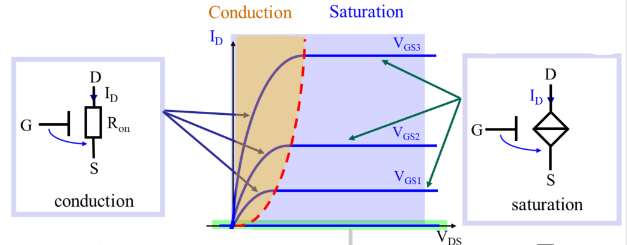
\includegraphics[width=.5\textwidth]{IMAGES/elec/Screenshot from 2023-12-11 13-51-52.png}
\end{figure}

Ainsi, en mode conduction, on a une résistance équivalente : \begin{equation}
    R_{on} = \frac{1}{\beta} \frac{1}{V_{GS}-V_T-0.5V_{DS}}
\end{equation}

\subsubsection{P-MOSFET}
Les tensions sont définies en sens opposé par rapport au NMOS; la source a le potentiel élevé et on met le semi-conducteur à $V_{cc}$.\\

\begin{figure}[hbt!]
    \centering
    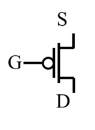
\includegraphics[width=.3\textwidth]{IMAGES/elec/Screenshot from 2023-12-11 13-54-40.png}
\end{figure}

Si $V_{SG} = V_{cc}$, pas de passage possible entre Drain et source, circuit ouvert.\\

Si $V_{SG}> V_T$, création d'un canal de type P conducteur entre drain et source.\\

Les équations pour régime saturation et linéaire sont les mêmes que pour le NMOS en changeant $V_{GS}$ avec $V_{SG}$ et $V_{DS}$ et $V_{SD}$.\\

\subsubsection{Application du MOSFET à l'analogique}

\quad \underline{Analyse des petits signaux :}\\
Une source continue en série avec une source sinusoïdale de faible amplitude. \\
La variation du courant de drain vis à vis de $V_{GS}$ est la transconductance de la grille : $g_m$.\\
\begin{equation}
    g_m = \frac{dI_D}{dV_{GS}} = \sqrt{2\beta I_D}
\end{equation}

Le gain en tension en mode saturation : \begin{equation}
    A_v = \frac{dV_{out}}{dI_D} \frac{dI_D}{dV_{in}} = -R_D \sqrt{2\beta I_D}
\end{equation}

\subsubsection{Logique CMOS}
Toute variable logique d'entrée a commande les deux grilles reliées d'une paire de transistors complémentaires, un NMOS et un PMOS.\\


\end{document}